% !TeX root = chapter2_1d.tex
% !TeX root = thesis.tex
\ifdefined\UtilIncluded
  \renewcommand{\startchapter}[1]{}
  \renewcommand{\stopchapter}{}
  \renewcommand{\undefinedlabel}[2]{}
\else

\newcommand{\startchapter}[1]{\begin{document}\setcounter{chapter}{#1}\addtocounter{chapter}{-1}}
\newcommand{\stopchapter}{\printbibliography[title=Bibliography,heading=bibintoc]\end{document}}


\documentclass{book}
\usepackage[utf8]{inputenc}


\usepackage{geometry}
\geometry{
  papersize={170mm,240mm},
}

\usepackage{amsfonts,amsmath, amsthm, amssymb, mathtools}
\usepackage{xspace}
\usepackage[hidelinks,bookmarks,pdfusetitle]{hyperref}
\usepackage{listings}
\usepackage[pdftex]{graphicx}
\usepackage{bm}
\usepackage[english]{babel}
\usepackage{caption}
\usepackage{subcaption}
\usepackage[usenames,dvipsnames]{xcolor}
\usepackage{physics}
\usepackage{multicol}
\usepackage{xstring}
\usepackage{pythonhighlight}
\usepackage{parskip}
\usepackage{thmtools}
\usepackage{relsize}
\usepackage{bookmark}
\usepackage{lmodern}
\usepackage{ifthen}
\usepackage{biblatex}
\usepackage{microtype}
\usepackage{csquotes}
\usepackage{numprint}
\usepackage{mleftright}
\npthousandsep{{\ifmmode\mskip2mu\else\hskip0.2em\fi}}
\npdecimalsign{.}

\addbibresource{references.bib}

\newtheorem{theorem}{Theorem}[chapter]
\newtheorem{lemma}[theorem]{Lemma}
\newtheorem{corollary}[theorem]{Corollary}
\newtheorem{definition}[theorem]{Definition}

\DeclareRobustCommand{\oneD}{{1{\relsize{-1}D}}\xspace}
\DeclareRobustCommand{\twoD}{{2{\relsize{-1}D}}\xspace}
\DeclareRobustCommand{\threeD}{{3{\relsize{-1}D}}\xspace}
\DeclareRobustCommand{\cpp}{{{C\nolinebreak[4]\hspace{-.05em}\raisebox{.4ex}{\relsize{-3}\textbf{++}}}\xspace}}
\pdfstringdefDisableCommands{%
  \def\cpp{C++}%
  \def\oneD{1D}%
  \def\twoD{2D}%
  \def\threeD{3D}%
}

\newcommand{\longchapter}[2][]{%
  \chapter[#2]{#2}%
  \ifthenelse{\equal{#1}{}}{}{\chaptermark{#1}}}

\newcommand{\NN}{\mathbb{N}}
\newcommand{\ZZ}{\mathbb{Z}}
\newcommand{\QQ}{\mathbb{Q}}
\newcommand{\QQbar}{\overline{\mathbb{Q}}}
\newcommand{\RR}{\mathbb{R}}
\newcommand{\CC}{\mathbb{C}}

\newcommand{\Eigen}{\texttt{Eigen}}

\newcommand{\sage}{\texttt{sage}\xspace}

\newcommand{\hamiltonian}{\mathcal{H}}

\newcommand{\transposesign}{\intercal}
\newcommand{\transpose}[1]{{#1}^\transposesign}
\newcommand{\adjointsign}{\text{H}}
\newcommand{\adjoint}[1]{{#1}^\adjointsign}

\newcommand{\xmin}{{x_{\text{min}}}}
\newcommand{\xmax}{{x_{\text{max}}}}
\newcommand{\ymin}{{y_{\text{min}}}}
\newcommand{\ymax}{{y_{\text{max}}}}

\newcommand{\Cbottom}{\vb{C}_\text{bottom}}
\newcommand{\Ctop}{\vb{C}_\text{top}}
\newcommand{\ubottom}{\vb{u}_\text{bottom}}
\newcommand{\utop}{\vb{u}_\text{top}}

\DeclareMathOperator{\diag}{diag}
\DeclareMathOperator{\tridiag}{tridiag}
\DeclareMathOperator{\eigs}{eigs}
\DeclareMathOperator*{\argmin}{arg\,min}
\DeclareMathOperator{\Ai}{Ai}
\DeclareMathOperator{\Bi}{Bi}
\DeclareMathOperator{\OO}{\mathcal{O}}

% https://tex.stackexchange.com/a/18192/163747
\makeatletter
\newcommand{\undefinedlabel}[2]{%
  \protected@write \@auxout {}{\string \newlabel {#1}{{#2}{\thepage}{#2}{#1}{}} }%
  \hypertarget{#1}{}
}
\makeatother

\fi
\gdef\UtilIncluded{}


\startchapter{2}
\undefinedlabel{cha:c3}{3}
\undefinedlabel{cha:c4}{4}
\undefinedlabel{sec:c3_calculate_vk}{3.x.x}

\longchapter[The \oneD Schrödinger equation]{The one-dimensional time-independent Schrödinger equation}\label{cha:c2}

\section{Introduction}

The one-dimensional time-independent Schrödinger equation is a linear ordinary differential equation posed as an eigenvalue problem on a domain $[a, b] \subseteq \RR$ with specified boundary conditions. Solutions are given as an eigenvalue $\lambda \in \RR$ with corresponding eigenfunction $y: \RR \to \RR$. These eigenfunctions are defined over the bounded domain $[a, b]$ of the problem. Each solution has to satisfy the following equation
$$
    -y''(x) + V(x)y(x) = \lambda y(x)
$$
for each of the values $x\in [a, b]$. In this equation the given function $V: \RR \to \RR$ is the potential of the problem at hand. Note that if $y(x)$ is an eigenfunction, $c\,y(x)$ will also be an eigenfunction with the same eigenvalue, for each value of $c \in \RR_0$. As such, it is not really possible to say ``\emph{the} eigenfunction corresponding to a certain eigenvalue". Later on we will prove that in many cases the eigenfunction is, up to a constant factor, uniquely defined.

Boundary conditions have to be specified before solutions can be found. These conditions pose restrictions on $y(a)$, $y'(a)$, $y(b)$ and $y'(b)$. Boundary conditions come in many flavors. We provide an overview of the most common ones:
\begin{itemize}
    \item \emph{Dirichlet boundary conditions} specify which value the solution takes on the boundary of the domain. In our case, eigenfunctions can always be scaled, as such, it is not useful to specify the value of the solution different from zero on the boundary. This type of boundary condition thus simplifies to $y(a) = 0$ and $y(b) = 0$, and is therefor called the homogeneous Dirichlet boundary conditions.
    \item \emph{Neumann boundary conditions} specify which value the derivative of a solution takes on the boundary of the domain. In our case, the same remark as given for the Dirichlet boundary conditions applies. This means that homogeneous Neumann boundary conditions imply that $y'(a) = 0$ and $y'(b) = 0$.
    \item \emph{Robin boundary conditions} are a generalization of both previous boundary conditions. When these conditions are imposed on a solution $y(x)$ we imply that a certain weighted average of the function and its derivative are a fixed value. In our case, homogeneous Robin boundary conditions can be imposed. This can be written as
          $$
              \alpha_a y(a) + \beta_a y'(a) = 0 \text{ and } \alpha_b y(b) + \beta_b y'(b) = 0  \text{.}
          $$
\end{itemize}
These three types of boundary conditions are what is called separated conditions. The condition on the left side $a$, or decoupled from the one on the right side $b$. In contrast, there are also boundary conditions that do coupled both ends.
\begin{itemize}
    \item \emph{Periodic boundary conditions} are used to specify that a solution should be periodic. In other words, the solutions has to end in the same value as it started, and so should the derivative. Mathematically this can be written as: $y(a) = y(b)$ and $y'(a) = y'(b)$. These condition can be extended to \emph{antiperiodic boundary conditions}: $y(a) = -y(b)$ and $y'(a) = -y'(b)$. Or even generalized with a $2 \times 2$ matrix $\vb{K}$:
          $$
              \begin{pmatrix} y(a) \\ y'(a) \end{pmatrix} = \vb{K} \begin{pmatrix} y(b) \\ y'(b) \end{pmatrix}\text{.}
          $$
\end{itemize}

Note that homogeneous Dirichlet or Neumann boundary conditions can always be written as homogeneous Robin boundary conditions. So when studying the one-dimensional time-independent Schrödinger equation it is more general to consider homogeneous Robin boundary conditions. Periodic (or generalized periodic) boundary conditions are less common and problems with these boundary conditions lose some of the nice properties which are guaranteed for separated conditions. This case will later be studied in section \ref{sec:c2_periodic}.

\subsection{Properties of the Sturm-Liouville equation}\label{sec:c2_slp_properties}

Before developing numerical methods for solving the one-dimensional time-independent Schrödinger equation, it is important to build a strong theoretical foundation. The goal is to build a thorough understanding of the Schrödinger equation and use this intuition to develop efficient and accurate numerical algorithms to solve this equation.

In the scientific literature it is quite rare to find studies about the one-dimensional Schrödinger equation itself. Most, if not all, relevant articles and books cover the more general topic of Sturm-Liouville theory. As Sturm-Liouville equations are a generalization of Schrödinger equations they are more widely applicable, and as such more useful to study. In this section, we will follow the tradition from the literature and study the Sturm-Liouville equation. Many more details and examples of Sturm-Liouville theory can be found in relevant textbooks, for example \cite[Chapter~5]{sagan_boundary_1961}.

The Sturm-Liouville equation is also a linear ordinary differential equation posed as a boundary value eigenproblem, given by the following equation on the bounded domain $[a, b]$:
\begin{equation}\label{equ:c2_sturm_liovuille_equation}
    -(p(x) y'(x))' + q(x) y(x) = \lambda w(x) y(x)\text{.}
\end{equation}
The functions $p(x)$, $q(x)$ and $w(x)$ are given on the domain $[a, b]$. These functions define the Sturm-Liouville problem. If $p(x)$, $q(x)$ and $w(x)$ are continuous, $p(x)$ is differentiable and $p(x) > 0$ and $w(x) > 0$ over the whole domain $[a, b]$, then the problem is called a \emph{regular} Sturm-Liouville problem.

A solution of a Sturm-Liouville problem consists of an eigenvalue $\lambda$ with corresponding eigenfunction $y(x)$, which satisfy \eqref{equ:c2_sturm_liovuille_equation} on $[a, b]$. For now, we will study the Sturm-Liouville equation with homogeneous Robin boundary conditions:
\begin{equation}\label{equ:c2_sturm_liovuille_boundary}
    \alpha_a y(a) + \beta_a p(a) y'(a) = 0 \text{ and } \alpha_b y(b) + \beta_b p(b) y'(b) = 0\text{.}
\end{equation}

Note that the Schrödinger equation with homogeneous Robin boundary conditions is a special case of the Sturm-Liouville equation: specifically, when $p(x) = 1$, $q(x) = V(x)$ and $w(x) = 1$.

Many theorems can be formulated about self-adjoint linear operators. For now, we provide a few specific theorems about Sturm-Liouville equations. The proofs for some of these theorems are quite extensive and require a thorough understanding of functional analysis. In this work, we will not provide these proofs.

For implementing methods to find solutions, it is valuable to study what a solution would look like. Since the solutions of a Sturm-Liouville problem are eigenvalues with corresponding eigenfunctions, solutions will consist of a possibly complex number $\lambda \in \CC$ with a corresponding function $y : [a, b] \to \CC$. The fact that these could be complex values impacts our study significantly. So, let us first prove that solutions can always be real.

\begin{theorem}\label{the:c2_real_eigenvalues}
    Let $p(x)$, $q(x)$ and $w(x)$ define a regular Sturm-Liouville problem on $[a, b]$.

    All eigenvalues of the Sturm-Liouville problem with real homogeneous Robin boundary condition \eqref{equ:c2_sturm_liovuille_boundary} are real. Corresponding eigenfunctions can always be scaled such that they are real.
\end{theorem}

Knowing we only need to find real solutions simplifies our work. The next theorem allows us to get a grasp on the number of eigenvalues we need to find.

\begin{theorem}\label{the:c2_slp_countable}
    The number of eigenvalues of a regular Sturm-Liouville problem with homogeneous Robin boundary conditions are countable. All eigenvalues have a lower bound, no upper bound and are unique. This implies that these can be written as:
    $$
        \lambda_0 < \lambda_1 < \lambda_2 < \dots \to \infty \text{.}
    $$

    We say that the $k^{\text{th}}$ eigenvalue $\lambda_k$ has \emph{index} $k$.
\end{theorem}

This last theorem is essential. It enables us to formulate questions such as: ``Find all eigenvalues less than $500$.'' or ``Find the first $10$ eigenvalues.'' Besides an eigenvalue, a solution also consists out of an eigenfunction.

\begin{theorem}
    With each eigenvalue $\lambda_k$, an up to scaling unique eigenfunction $y_k : [a, b] \to \RR$ is associated. Eigenfunctions corresponding to different eigenvalues are orthogonal with respect to the weight function $w(x)$:
    $$
        \int_a^b y_m(x) y_n(x) w(x) \, \dd x = 0 \quad \text{ if $m \neq n$.}
    $$
\end{theorem}

\begin{figure}
    \begin{center}
        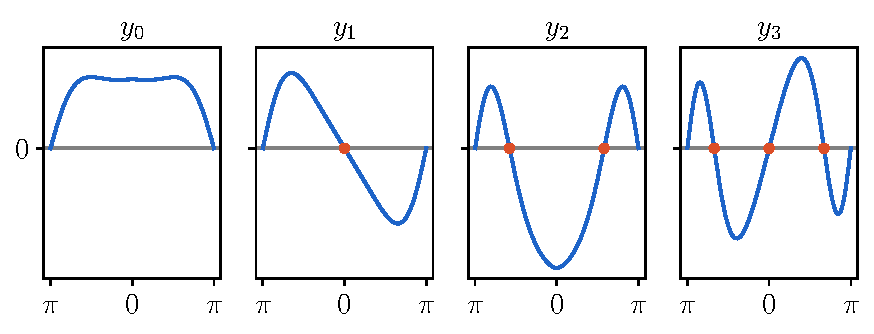
\includegraphics[width=\textwidth]{img/chapter2/slp_count_roots.pdf}
    \end{center}
    \caption{The first four eigenfunctions of the Sturm-Liouville problem with $p(x) = 1$, $q = \sqrt{|x|}$, $w(x) = 1+x^2$ and homogeneous Dirichlet boundary conditions on $[-\pi, \pi]$. The roots of each of these functions are indicated.}
    \label{fig:c2_sturm_liovuille_k_roots}
\end{figure}

Even stronger: Sturm-Liouville theory provides a way to characterize the index of an eigenvalue by means of only the eigenfunction.

\begin{theorem}\label{the:c2_kth_eigen_k_roots}
    The eigenfunction $y_k(x)$ corresponding to the $k^{\text{th}}$ eigenvalue $\lambda_k$ has exactly $k$ zeros in the interior of the domain $\left]a, b\right[$.
\end{theorem}

This theorem is illustrated in figure \ref{fig:c2_sturm_liovuille_k_roots}. Here we see the first few eigenfunctions of a Sturm-Liouville problem. Later on we will use the term ``highly oscillatory eigenfunction'', theorem \ref{the:c2_kth_eigen_k_roots} explains why this is justified. If $k$ becomes large, the eigenfunction will have many zeros and therefor will oscillate heavily. This can also already be seen on the last panel of figure \ref{fig:c2_sturm_liovuille_k_roots}.

With these four theorems in the back of our minds we will be able to develop numerical methods for solving Sturm-Liouville and Schrödinger problems. As stated in the beginning of this section, we have given a very brief overview of the for us relevant theorems. If the reader is interested in more details, or a rigorous theoretical framework many textbooks are available, for example \cite{sagan_boundary_1961,al-gwaiz_sturmliouville_2008,zettl_sturmliouville_2012,guenther_sturmliouville_2018}.

Throughout this thesis, and the research preceding it, we have not and will not focus on the applicability of the Sturm-Liouville equation. This is definitely not due to a lack of applications. Rather, the opposite: Sturm-Liouville equations pop up in an innumerable diversity of fields. Many real-world problems can be stated as or reduced to differential equations and in particular the Sturm-Liouville equation.

\todo{Give some real-world examples of this equation \cite[Chapter~8]{guenther_sturmliouville_2018}.}

\subsection{Liouville's transformation}\label{sec:c2_liouville_transformation}
\todo{Formulae, and some notes about implementing it, refer to Veerle's thesis.}

Liouville provided, under certain conditions, a transformation to reduce the Sturm-Liouville equation back to the Schrödinger equation. This transformation can be used to employ the easier numerical algorithms for Schrödinger equations, to solve more general Sturm-Liouville equations.

\section{Background about Matslise}\label{sec:c2_background}

Numerical methods for ordinary differential equations as \emph{initial value} problems are already many centuries old, starting with Euler's method. Numerical methods as a research topic by itself really took of a little more than a century ago. In particular, linear multistep methods and Runge-Kutta methods were described around 1900. First they were applied and calculated by hand, later on ``calculating machines'' \cite{milne_numerical_1926} were used. Nowadays, modern computers do all the tedious computations.

For ordinary differential equations as \emph{boundary value} problems, such as the Sturm-Liouville equations, the story is different. There still are only a few general methods for such problems. For linear ordinary differential equations, one of the more popular choices is a method based upon finite differences.

\begin{figure}
    \begin{center}
        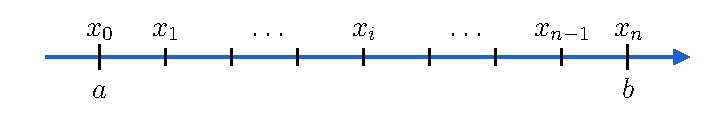
\includegraphics[width=\textwidth]{img/chapter2/finite_difference_grid.pdf}
    \end{center}
    \caption{An equidistant division of the domain $[a, b]$ in $n$ intervals.}
    \label{fig:c2_finite_difference_grid}
\end{figure}

To illustrate the idea behind methods based upon finite difference, consider the linear second order differential equation
$$
    y''(x) = \alpha + \beta y(x) + \gamma y'(x)
$$
on the interval $[a, b]$ with boundary conditions $y(a) = y_a$ and $y(b) = y_b$. First, we discretize the integration domain $[a, b]$ into an equally spaced grid of points $a = x_0$, $x_1$, $\dots$, $x_i$, $\dots$, $x_{n-1}$, $x_{n} = b$, with $\Delta x$ the distance between two consecutive points. This discretization can be seen in figure \ref{fig:c2_finite_difference_grid}. The differential equation is now approximated by using finite difference expressions of the involved derivatives. For example:
\begin{align*}
    y''(x_i)            & \approx \frac{y(x_{i-1}) - 2 y(x_i) + y(x_{i+1})}{\Delta x^2} \\
    \text{and } y'(x_i) & \approx \frac{y(x_{i+1}) - y(x_{i-1})}{2 \Delta x}\text{.}
\end{align*}
This simplification yields a linear system in the variables $y(x_1), \dots, y(x_{n-1})$. In general, for linear ordinary differential equations with linear boundary conditions, this technique leads to a linear matrix-vector reformulation of the differential equation, which can be solved with classical linear algebra tools.

In this general technique constructing higher order methods is mostly as straightforward as using a more accurate finite difference approximation. But these methods become increasingly computationally expensive as more accuracy is required. Or in our case, if an eigenvalue problem is being solved, when higher eigenvalues are requested, computational cost increases significantly.

\subsubsection{Finite difference scheme for the Sturm-Liouville equation}

Until around 1990 the best methods \cite{andrew_correction_1985,vandenberghe_accurate_1991} for approximating solutions to the Sturm-Liouville problem looked at the simpler form of the Schrödinger equation and employed a finite difference scheme. After solving the approximating linear algebra problem, they applied some corrections to improve the accuracy of higher eigenvalues. They experimented with which finite difference approximations to use. First they tried classical formulae, later on highly tuned exponential fitted formulae to better handle the oscillatory nature of the eigenfunctions were developed.

To illustrate this class of finite difference methods for Sturm-Liouville equations we will develop a simple version ourselves. This will allow us to appreciate the nuances of these methods more, and it will give us some ideas about the general advantages but also disadvantages of this technique. For completeness, we recall the Sturm-Liouville equation from \eqref{equ:c2_sturm_liovuille_equation}:
$$
    -(p(x)y')' + q(x) y = \lambda w(x) y\text{.}
$$
In this example we will approximate solution to this equation on the interval $[a, b]$ and impose homogeneous Dirichlet boundary conditions $y(a) = y(b) = 0$. As stated earlier, solutions will consist of eigenvalues $\lambda$ and corresponding eigenfunctions $y(x)$.

As a first step we discretize the domain $[a, b]$ with $n+1$ equidistant points, as in figure \ref{fig:c2_finite_difference_grid}. The eigenfunctions $y(x)$ we are looking for, can now be approximated by values in each of the grid points $y(x_i) \approx y_i$. For translating this problem into a linear matrix-vector equation, we are missing one key component. We need a way to discretize the expression $(p(x) y')'$. For this, we apply the central second order finite difference formula for the first derivative twice, with half the step size. In more detail, the first derivative of a scalar function $f(x)$ can be approximated as:
$$
    f'(x) \approx \frac{f(x + h) - f(x - h)}{2h}\text{.}
$$

Applying this expression once to $(p(x) y')'$ in the point $x_i$, with step size $h = \frac{\Delta x}{2}$ gives:
$$
    (p(x) y')'(x_i) \approx \frac{1}{\Delta x}\left((p y')\left(x_{i+\frac{1}{2}}\right) - (p y')\left(x_{i-\frac{1}{2}}\right))\right)\text{.}
$$
Applying the finite difference formula a second time, with step size $\frac{\Delta x}{2}$ to approximate $y'(x)$ yields:
$$
    (p(x) y')'(x_i) \approx \frac{1}{\Delta x^2}\left(p_{i+\frac{1}{2}} y_{i+1} - \left(p_{i-\frac{1}{2}} + p_{i+\frac{1}{2}}\right) y_i + p_{i-\frac{1}{2}} y_{i-1}\right)
$$
To ease notation we have substituted $y(x_i)$ with its approximation $y_i$, and have denoted $\frac{x_i + x_{i+1}}{2}$ as $x_{i+\frac{1}{2}}$, and $p(x_i)$ as $p_i$. Also, note that if $p(x) = 1$ this formula simplifies to the classical, well-known, central second order approximation of the second derivative.

If we apply this finite difference approximation to \eqref{equ:c2_sturm_liovuille_equation} in each point $x_i$, then we get the linear generalized eigenvalue problem:
$$
    -\frac{1}{\Delta x^2}\left(p_{i+\frac{1}{2}} y_{i+1} - \left(p_{i-\frac{1}{2}} + p_{i+\frac{1}{2}}\right) y_i + p_{i-\frac{1}{2}} y_{i-1}\right) + q(x_i) y_i = \lambda w(x_i) y_i \text{.}
$$

To emphasize that this is a linear algebra problem we can rewrite this in matrix notation:
\begin{equation}\label{equ:c2_finite_difference_matrix_problem}
    \left(-\vb{T} + \diag(\vb{q})\right)\vb{y} = \lambda \diag(\vb{w}) \vb{y}\text{.}
\end{equation}

The $(n-1)$-dimensional vector $\vb{y} = \transpose{\begin{pmatrix}y_1 & y_2 & \dots & y_{n-1}\end{pmatrix}}$ is the unknown approximation of the eigenfunction. The $(n-1)$-dimensional vectors $\vb{q} = \transpose{\begin{pmatrix}q(x_1) & q(x_2) & \dots & q(x_{n-1})\end{pmatrix}}$  and $\vb{w} = \transpose{\begin{pmatrix}w(x_1) & w(x_2) & \dots & w(x_{n-1})\end{pmatrix}}$ are the values of the coefficient functions $q$ and $w$. And lastly, the matrix $\vb{T}$ is the tridiagonal matrix given by:
$$
    \vb{T} = \frac{1}{\Delta x^2}\begin{pmatrix}
        -p_{\frac{1}{2}} -p_{\frac{3}{2}} & p_{\frac{3}{2}}                   &                                   &                     &                                            \\
        p_{\frac{3}{2}}                   & -p_{\frac{3}{2}} -p_{\frac{5}{2}} & p_{\frac{5}{2}}                   &                     &                                            \\
                                          & p_{\frac{5}{2}}                   & -p_{\frac{5}{2}} -p_{\frac{7}{2}} & p_{\frac{7}{2}}     &                                            \\
                                          &                                   &                                   & \ddots              &                                            \\
                                          &                                   &                                   & p_{n - \frac{3}{2}} & -p_{n - \frac{3}{2}} - p_{n - \frac{1}{2}} \\
    \end{pmatrix}{}\text{.}
$$

To find the eigenvalues of \eqref{equ:c2_finite_difference_matrix_problem} one can notice that if $w(x_i)$ is never $0$ for $0 < i < n$ then $\diag(\vb{w})$ is invertible and the problem becomes a simple tridiagonal eigenvalue problem. This can then be solved with any of our favorite tridiagonal eigenvalue solvers. If $w$ happens to be constant, this becomes a symmetric tridiagonal matrix, for which LAPACK \cite{lapack}, for example, contains the specialized routines \texttt{?stev} and relatives.

\begin{figure}
    \begin{center}
        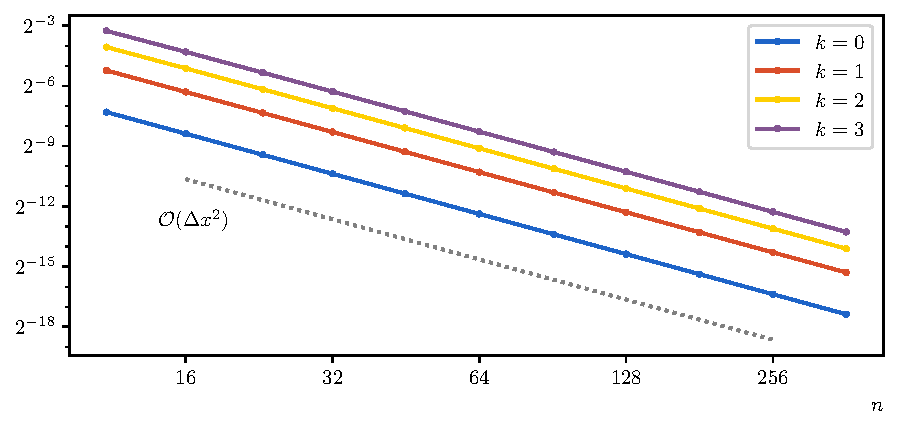
\includegraphics[width=\textwidth]{img/chapter2/finite_difference_h_error.pdf}
    \end{center}
    \caption{Relative error of approximated eigenvalues of problem \eqref{equ:c2_fd_test_problem} in function of the number of grid points $n+1$ on the domain.}
    \label{fig:c2_fd_h_error}
\end{figure}

\begin{figure}
    \begin{center}
        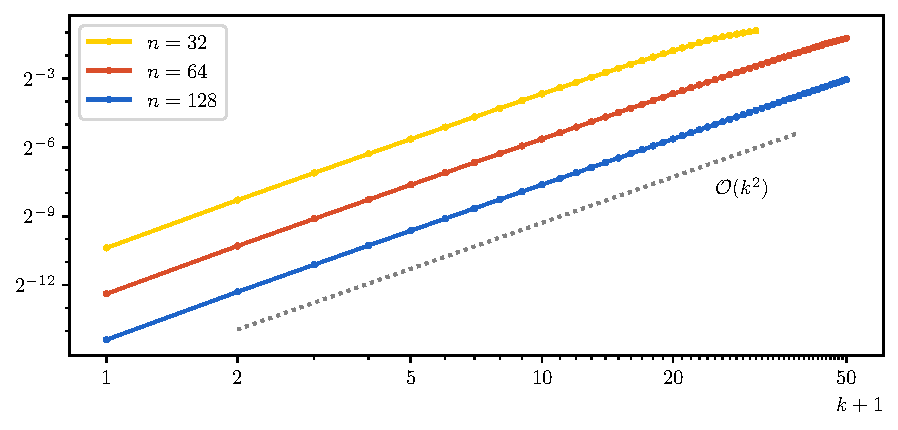
\includegraphics[width=\textwidth]{img/chapter2/finite_difference_k_error.pdf}
    \end{center}
    \caption{Relative error of approximated eigenvalues of problem \eqref{equ:c2_fd_test_problem} in function of the eigenvalue index $k$.}
    \label{fig:c2_fd_k_error}
\end{figure}

As a numerical experiment of this method we will take a look at the following Sturm-Liouville equation:
\begin{equation}\label{equ:c2_fd_test_problem}
    -\left((1+x)^2 y \right)' + (x^2 - 2) y = \lambda e^x y
\end{equation}
on the domain $[0, 1]$ with homogeneous Dirichlet boundary conditions. Figure \ref{fig:c2_fd_h_error} shows the relative errors of the 4 lowest eigenvalues in function of the chosen number of grid points $n+1$. As $n$ increases, the error decreases, as desired. Notice that as the constructed method is based upon second order finite difference formulae, we expect to see the decrease of error be of second order too. This is indicated in the figure with the dotted line. The constructed method is of relatively low order, so to compute very accurate approximations, a dense grid is needed. In the literature one can find many methods based upon finite difference approximations, many of which use (much) higher order formulae. These better methods can reach high accuracy with relatively little computational work for the first few eigenvalues.

As earlier hinted, methods based upon finite differences struggle with the computation of higher eigenvalues. Figure \ref{fig:c2_fd_k_error} illustrates this. Here, the relative error of the first 50 eigenvalues is plotted, for different values of $n$. Note that in the case of $n = 32$, only $32$ eigenvalues can be computed. On this figure, the line corresponding to $\mathcal{O}(k^2)$ is drawn. Together with the $\mathcal{O}(\Delta x^2)$ from earlier, one expects the relative error of the $k^\text{th}$ eigenvalue to be
$$
    \mathcal{O}(\Delta x^2 k^2)
$$
for this method applied to problem \eqref{equ:c2_fd_test_problem}. This shows us that the larger the eigenvalue, the more difficult it is to compute accurately. This lesson not only holds for this method in particular, but it is also applicable to most methods of this type. In the literature one can find some techniques to mitigate this effect by applying some corrections after the fact. In \cite{andrew_correction_1985} such a correction is analyzed when applied to Numerov's method. Here, the authors are able to bring the error down from $\mathcal{O}(k^6 h^4)$ to $\mathcal{O}(k^3 h^4)$. This is remarkably better. But even with this correction technique, computing large eigenvalues is still computationally difficult.

\subsection{CP-methods}

The drawbacks of the methods based upon finite differences are already known for a long time. One of the first\footnote{In \cite{ledoux_solving_2010} a brief historical overview is given of the application of CP-methods to Sturm-Liouville problems. In this thesis we will take the time to take a closer look at the earlier methods. They will provide us a more intuitive understanding of the algorithms, in preparation of our own advancements within employing these ideas.} works that tries to not only mitigate these troubles but rather fully fix them, was \cite{canosa_new_1970} in 1970. There, Canosa and De Oliveira present a new method to approximate solutions to the one dimensional time-independent Schrödinger equation. Here, the foundations are build to what would later be called constant perturbation methods (CPM or CP-methods). To intuitively appreciate these CP-methods it is valuable to study the method from \cite{canosa_new_1970}.

For this, we will only consider the Schrödinger equation
\begin{equation}\label{equ:c2_cpm_schrodinger}
    - y'' + V(x) y = \lambda y
\end{equation}
on the domain $[a, b]$ with homogeneous Robin boundary conditions $\alpha_a y(a) + \beta_a y(a) = 0$ and $\alpha_b y(b) + \beta_b y(b) = 0$. But do note, that using Liouville's transformation Sturm-Liouville problems can be transformed into Schrödinger problems.

\subsubsection{Piecewise constant approximation of the potential}

\begin{figure}
    \begin{center}
        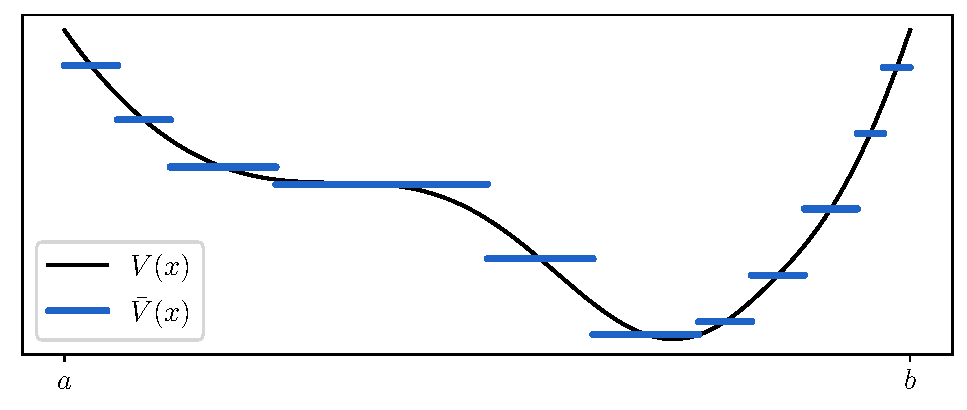
\includegraphics[width=\textwidth]{img/chapter2/cpm_constant_approx.pdf}
        \caption{A potential function $V(x)$ is approximated as the piecewise constant function $\bar{V}(x)$ along the domain $[a, b]$.}
        \label{fig:c2_cpm_constant_approx}
    \end{center}
\end{figure}

As a very first step, \cite{canosa_new_1970} simplifies the potential $V(x)$ as a piecewise constant approximation $\bar{V}(x)$. This approximation is visualized in figure \ref{fig:c2_cpm_constant_approx}. Notice that no restrictions are placed upon the size of the subintervals, and a non-uniform grid is definitely allowed. Upon choosing $\bar{V}(x)$, one should keep in mind that the better the piecewise approximation is, the better the resulting eigenvalues will be. Also, the computational runtime depends linearly on the number of subintervals used.

The next step is to fix the value for $\lambda$ for now. Then, for each subinterval $[x_i, x_{i+1}]$ the potential is approximated $V_i \approx V(x)$ for $x \in [x_i, x_{i+1}]$. With this approximation, the analytical solution is computed of the problem
$$
    y'' = (V_i - \lambda) y\text{.}
$$
These analytical solutions $y_i(x)$ have the following structure.
$$
    y_i(x) = \begin{cases}
        A_i + B_i x                                                         & \text{ if $V_i = \lambda$} \\
        A_i \cos(x\sqrt{\lambda - V_i}) + B_i \sin(x\sqrt{\lambda - V_i})   & \text{ if $V_i < \lambda$} \\
        A_i \cosh(x\sqrt{V_i - \lambda}) + B_i \sinh(x\sqrt{V_i - \lambda}) & \text{ if $V_i > \lambda$}
    \end{cases}
$$

To determine the appropriate values for $A_i$ and $B_i$ continuity conditions at the grid points are applied:
$$
    y_{i-1}(x_i) = y_{i}(x_i) \text{ and } y_{i-1}'(x_i) = y_{i}'(x_i) \text{.}
$$
If $n$ subintervals are used, this system of equations has $2n$ variables and $2(n-1)$ equations. Together with the two equations from the boundary conditions, this yields a fully determined linear system. Now, we have translated the problem of finding eigenvalues of the Schrödinger equation \eqref{equ:c2_cpm_schrodinger} to finding values for $\lambda$ such that this system of equations has non-zero solutions. Only these solutions correspond to a non-zero eigenfunction.

Finding values for $\lambda$ for which the constructed system becomes singular is not as trivial as one may assume. In \cite{canosa_new_1970}, the authors have provided their own root finding algorithm based upon finding changes in the sign of the determinant. But this algorithm is not without issue. Eigenvalues may be arbitrarily close together, which makes it hard to ensure you have found all requested values. Choosing the appropriate step sizes when eigenvalues become increasingly sparse is a balance between efficiency and not missing any. Later on we will describe a way to reliably and efficiently determine all required eigenvalues.

One of the main benefits of this ``new method for the solution of the Schrödinger equation'' \cite{canosa_new_1970} is that its accuracy does not depend on the size of the requested eigenvalue. Because only analytical solutions of the piecewise approximated problem are considered, oscillations can be represented exactly. Even the most extreme oscillations are cleanly captured inside the $\sin$ en $\cos$ of $y_i$. The idea of using analytical solutions allowed the development of the CP-methods.

When studying this method one can make the observation when looking at figure \ref{fig:c2_cpm_constant_approx} that $\bar{V}(x)$ is a crude approximation of the function $V(x)$. The importance of this remark becomes even more apparent when one realizes that the accuracy of the method solely depends upon the accuracy of this approximation.

Nonetheless, the idea of Canosa and De Oliveira gained traction. In 1971 Ixaru \cite{ixaru_error_1972} has written a note about the error analysis of this new method. And in the same year Pruess \cite{pruess_estimating_1973} has studied this method thoroughly and provided numerical examples of linear piecewise approximations and quadratic piecewise approximations of the potential function. Due to this analysis this is now known as Pruess's method.

Here we will state the most important theorems from \cite{pruess_estimating_1973}, without proof. All details can be found in the original work.

\begin{theorem}[Pruess 1973]\label{the:c2_pruess_1973_1}
    Let $\lambda_k$ be the $k^\text{th}$ eigenvalue of the Schrödinger equation
    $$
        -y'' + V(x) y = \lambda y
    $$
    on the domain $[a, b]$ with homogeneous Robin boundary conditions. And let $\tilde{\lambda}_k$ be the $k^\text{th}$ eigenvalue of the approximate Schrödinger equation with potential $\bar{V}(x)$ on the same domain, with identical boundary conditions. Here $\bar{V}(x)$ is a piecewise $m^\text{th}$ degree polynomial approximation, let $h$ be the width of the largest subinterval in this approximation. For $h$ sufficiently small, we have as $h \to 0$,
    $$
        |\lambda_k - \tilde{\lambda}_k| = \mathcal{O}(h^{2m + 2}) \text{ for each $k$.}
    $$
\end{theorem}

This theorem provides justification for the idea of Canosa and De Oliveira. Even though a constant approximation ($m = 0$) may be crude, it still is a second order method. Furthermore, the theorem suggest that expanding this method up to higher degree piecewise polynomial approximations may be worthwhile.

In \cite{pruess_estimating_1973}, the author also studies what happens to the error on the eigenvalues if $k$ is increased. In \cite{canosa_new_1970} it was assumed that this error does not get worse as $k$ increases.

\begin{theorem}[Pruess 1973]\label{the:c2_pruess_1973_2}
    Following the notation from theorem \ref{the:c2_pruess_1973_1}, assume $\bar{V}(x)$ to be a least squares $m^\text{th}$ degree piecewise polynomial approximation of $V(x)$, i.e.~on each subinterval $[x_i, x_{i+1}]$, $\bar{V}$ is the $m^\text{th}$ degree polynomial such the following is minimal
    $$
        \int_{x_i}^{x_{i+1}} \left(V(x) - \bar{V}(x)\right)^2 \dd x \text{.}
    $$

    Under this assumption, if $k \to \infty$, it holds for the relative error that
    $$
        \frac{\lambda_k - \tilde{\lambda}_k}{\lambda_k} = \mathcal{O}(k^{-4})\text{.}
    $$
\end{theorem}

This last theorem does not only say that the error does not become larger if $k$ increases, but the relative error even decreases rapidly when $k \to \infty$. Theorem \ref{the:c2_pruess_1973_2} highlights the main advantage this technique has in comparison to other state-of-the-art methods. Where many other methods become less and less accurate for large eigenvalues, this method becomes even more accurate.

\begin{figure}
    \begin{center}
        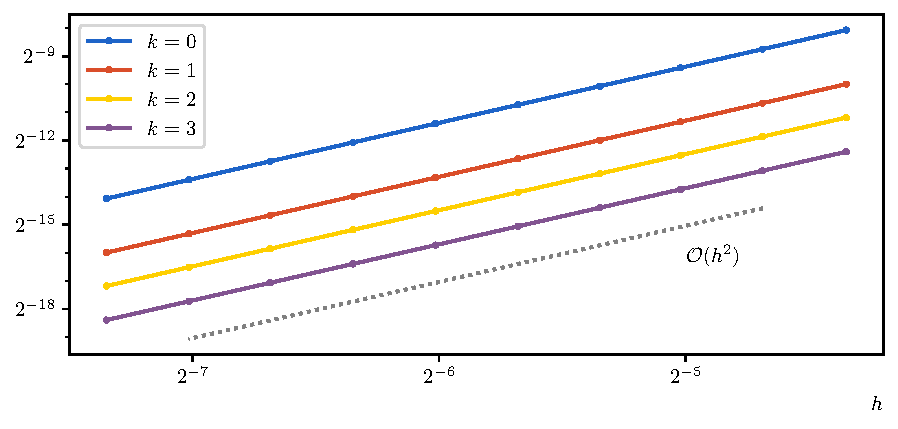
\includegraphics[width=\textwidth]{img/chapter2/pruess_h_error.pdf}
    \end{center}
    \caption{Relative error of the found eigenvalues of problem \eqref{equ:c2_pruess_test_problem} by using the method of constant piecewise approximation of the potential on a uniform mesh with step size $h$. The most accurate calculation used $512$ subintervals, the least accurate $64$.}
    \label{fig:c2_pruess_h_error}
\end{figure}

\begin{figure}
    \begin{center}
        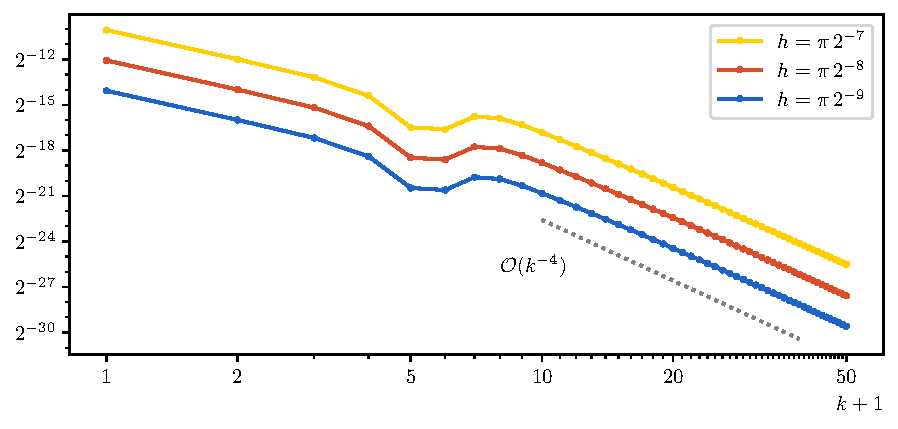
\includegraphics[width=\textwidth]{img/chapter2/pruess_k_error.pdf}
    \end{center}
    \caption{Relative error of the found eigenvalues of problem \eqref{equ:c2_pruess_test_problem} by using the method of constant piecewise approximation of the potential on a uniform grid with step size $h$. The graphs are in function of the index of the eigenvalue. The yellow line used $128$ subintervals, the blue line $512$.}
    \label{fig:c2_pruess_k_error}
\end{figure}

As a numerical experiment we have applied the method with constant piecewise approximations ($m=0$) to the problem
\begin{equation}\label{equ:c2_pruess_test_problem}
    -y'' + 100 \cos^2(x) \,y = \lambda y
\end{equation}
on the domain $[0, \pi]$ with homogeneous Dirichlet boundary conditions. In figure \ref{fig:c2_pruess_h_error} the relative error of the application of the method is illustrated. We see that the error follows indeed the predicted line of $\mathcal{O}(h^2)$. In figure \ref{fig:c2_pruess_k_error} we see the dramatic increase in accuracy when $k$ becomes larger. The predicted order of $\mathcal{O}(k^{-4})$ seems to be reached once $k$ is sufficiently large.


But still some nuances have to be made. In \cite{pruess_estimating_1973} some numerical examples are given for constant ($m=0$), linear ($m=1$) and quadratic ($m=2$) approximations. But only for the constant approximations analytical solutions were used. For the higher order experiments, the true solution on a single subinterval is approximated by an at least fifteenth order Taylor series expansion. These Taylor series are only polynomial approximations of a possibly highly oscillatory function. This will give problems for higher lying eigenvalues.

\subsubsection{Constant perturbation methods}

In the years since the first article from Canosa and De Oliveira \cite{canosa_new_1970}, the research into these kinds of methods has flourished. One of the first extensions considered not only piecewise constant approximations but also linear and quadratic approximations, as in \cite{pruess_estimating_1973}. For constant approximations, the exact solution is given by hyperbolic or trigonometric functions. For linear approximations, the Airy functions $\Ai(x)$ and $\Bi(x)$ are appropriate. As these are well-known special functions, software packages are available to evaluate them. But not unexpectedly, these packages are harder to find, and more difficult to use, than sine, cosine, and hyperbolic variants. For quadratic, and higher order, approximations no closed form formula exists for the exact solutions.

To improve accuracy and computational efficiency, it is, when developing numerical methods, valuable to construct higher order methods. As we are limited to an order of $\mathcal{O}(h^2)$ for constant approximations, or $\mathcal{O}(h^4)$ when using linear approximations, some alternative improvements were required. In the book \cite{ixaru_numerical_1984}, Ixaru dedicated chapter 3 to the development of the constant perturbation methods. The main idea is to not directly improve the approximation of $V(x)$, but starting with a piecewise constant approximation $\bar{V}(x)$, adding correction terms to capture the difference between the reference solution for $\bar{V}(x)$ and the true solution for $V(x)$.

Before we analyze the constant perturbation methods, let us take the time to formalize which mathematical problem we are solving. For now, we will only look at the differential equation
\begin{equation}\label{equ:c2_cpm_corrected}
    y''(\delta) = (\Delta V(\delta) + \bar{V} - \lambda) y(\delta)
\end{equation}
as initial value problem starting from $0$. Denote the homogeneous Neumann solution as $u(\delta)$, as such, $u(0) = 1$ and $u'(0) = 0$. And, we will write the homogeneous Dirichlet solution as $v(\delta)$, thus $v(0) = 0$ and $v'(0)=1$. In \eqref{equ:c2_cpm_corrected}, $\bar{V}$ is a constant (not piecewise) approximation of $V(x)$ on the current subinterval $[x_i, x_{i+1}]$ and $\Delta V(\delta) := V(x_i + \delta) - \bar{V}$. Being able to solve the initial value problem is sufficient to also solve the boundary value eigenproblem. For solving the latter we can employ a shooting procedure to the former, see section \ref{sec:c2_shooting_prufer} for more details. The procedure we will develop here can then be applied to each of the subintervals in the constant piecewise approximation of $V(x)$.

Following \cite{ixaru_numerical_1984,ixaru_cp_2000}, let us denote a solution of \eqref{equ:c2_cpm_corrected} generally as $p(\delta)$, this thus represents either $u(\delta)$ or $v(\delta)$. Now we write the solution $p(\delta)$ as a perturbation series:
$$
    p(\delta) = p_0(\delta) + p_1(\delta) + p_2(\delta) + \dots
$$
In this expression the first order term $p_0$ is the solution of the reference equation
\begin{equation}\label{equ:c2_p0_reference}
    p_0''(\delta) = (\bar{V} - \lambda) p_0(\delta)
\end{equation}
with appropriate initial values. That is, $u_0(0) = 1$ and $u_0'(0) = 0$ for $p = u$, if $p=v$ the initial values are $v_0(0)=0$ and $v_0'(0) = 1$. The perturbation corrections can now be recursively defined as the solution of
\begin{equation}\label{equ:c2_pq_definition}
    p_q''(\delta) = (\bar{V} - \lambda) p_q(\delta) + \Delta V(\delta) p_{q-1}
\end{equation}
with initial conditions $p_q(0) = p_q'(0) = 0$. Notice that this definition implies that $p$ indeed solves \eqref{equ:c2_cpm_corrected} with the appropriate initial values:
\begin{align*}
    p'' & = (\bar{V} - \lambda)p_0 + \sum_{q=1}^\infty\left((\bar{V} - \lambda)p_q + \Delta V(\delta) p_{q-1}\right) \\
        & = (\bar{V} - \lambda)\sum_{q=0}^\infty p_q + \Delta V(\delta) \sum_{q=0}^\infty p_q                        \\
        & = (\Delta V(\delta) + \bar{V} - \lambda)p\text{.}
\end{align*}

To symbolically compute the expression of $p_q$ Ixaru has introduced some auxiliary functions\footnote{What we will call $\eta_{-1}$, Ixaru has named $\xi$. The notation of the recursive definition becomes a little easier when the $\eta_m$ and $\xi$ names are unified.}, based upon the analytical solution of equation \eqref{equ:c2_p0_reference}.

\begin{definition}[Ixaru 1984]\label{def:c2_eta_functions}
    The family of $\eta$-functions $\eta_m : \RR \to \RR$ for $m \in \{-1, 0, 1, \dots\}$ is defined recursively as:
    \begin{align*}
        \eta_{-1}(Z) & = \cosh(\sqrt{Z})                                        \\
        \eta_{0}(Z)  & = \frac{\sinh(\sqrt{Z})}{\sqrt{Z}}                       \\
        \eta_{m}(Z)  & = \frac{\eta_{m-2}(Z) - (2m-1) \eta_{m-1}(Z)}{Z}\text{.}
    \end{align*}
    When $Z < 0$ the definitions of $\eta_{-1}$ and $\eta_{0}$ should be read as calculations in $\CC$. But, notice that the resulting values will always be real. Furthermore, if $Z = 0$, one should take the limit of $\eta_m$ to zero, this yields\footnote{In this expression $n!!$ is the double factorial: $n!! := n\cdot (n-2) \cdot (n - 4) \cdot ...$, with only strictly positive integers as factors. For our purposes we define $0!! = (-1)!! = 1$.} $\eta_m(0) = \frac{1}{(2m+1)!!}$.
\end{definition}

\begin{figure}
    \begin{center}
        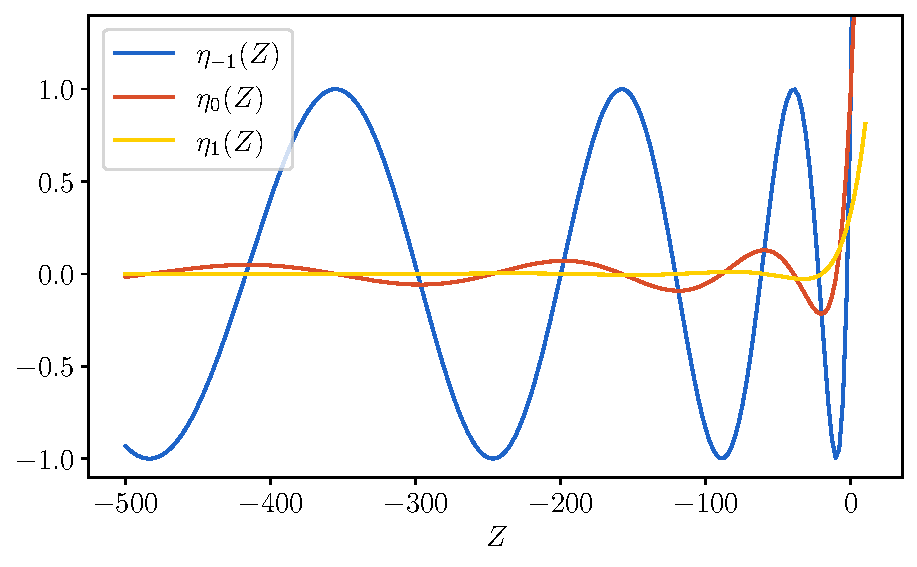
\includegraphics[width=\textwidth]{img/chapter2/eta_functions.pdf}
    \end{center}
    \caption{A graph of the first three $\eta$-functions.}\label{fig:c2_eta_functions}
\end{figure}

Much has already been written about these instrumental functions. For example in Ixaru's book \cite{ixaru_numerical_1984}. To get a feeling for these functions, we provide figure \ref{fig:c2_eta_functions}.

In definition \ref{def:c2_eta_functions}, we have chosen to simplify the notation by allowing computations in $\CC$. But when implementing these formulas, it is much more efficient to keep all calculations in $\RR$. For $Z < 0$, we implement $\eta_{-1}(Z) = \cos(\sqrt{-Z})$ and $\eta_{-1}(Z) = \sin(\sqrt{-Z})/\sqrt{-Z}$.

Another interesting property of these $\eta$-functions is its series expansions:\begin{align*}
    \eta_{-1}(Z) & = \sum_{q=0}^{\infty} \frac{Z^q}{(2q + 1)!}                                                      \\
    \eta_{m}(Z)  & = 2^m \sum_{q=0}^{\infty} \frac{(q+m)! Z^q}{q!(2q + 2m + 1)!} \qquad \text{if } m \geq 0\text{.}
\end{align*}
When $|Z|$ is small, the recursion from the definition becomes numerically unstable. It is more accurate to use this series expansion on $\eta_m$ and $\eta_{m+1}$, for $m$ sufficiently large, and work our way back to $m=0$ and $m=-1$ with the inverted recursion
$$
    \eta_{m-1}(Z) = Z \eta_{m+1}(Z) + (2 m + 1) \eta_{m}(Z)
    \text{.}
$$

Other interesting properties of these special functions are already studied. Here we provide some results, without proofs.
\begin{theorem}[Ixaru 1984]\label{the:c2_eta_functions}
    For the family of functions defined in definition \ref{def:c2_eta_functions}, the following properties hold for $m \in \{-1, 0, 1, 2, \dots\}$ and $Z \in \RR$.
    \begin{itemize}
        \item Asymptotic behavior for $|Z| \to \infty$:
              $$\eta_m(Z) \approx  \begin{dcases}
                      \frac{\eta_{-1}(Z)}{Z^{(m+1)/2}} & \text{if $m$ is odd}  \\
                      \frac{\eta_{0}(Z)}{Z^{m/2}}      & \text{if $m$ is even}
                  \end{dcases}$$
        \item Differentiation with respect to $Z$:
              $$
                  \eta'_{m}(Z) = \frac{1}{2}\eta_{m+1}(Z)
              $$
        \item Differentiation with respect to $\delta$ if $Z = F\delta^2$:
              \begin{align*}
                  \pdv[]{\eta_{-1}(Z)}{\delta}             & = \frac{Z}{\delta} \eta_0(Z)                           \\
                  \pdv[]{\delta^{2m+1}\eta_{m}(Z)}{\delta} & = \delta^{2m} \eta_{m-1}(Z) \qquad \text{if } m \geq 0 \\
              \end{align*}
    \end{itemize}
\end{theorem}

With the theory about the family of $\eta$-functions in hand, we are able to solve equations \eqref{equ:c2_p0_reference} and \eqref{equ:c2_pq_definition} symbolically. The following theorem from \cite{ixaru_numerical_1984} captures these symbolic calculations for $p_q(\delta)$. As these formulae have been instrumental to our work (especially for section \ref{sec:c2_cp_in_delta}), we will provide a proof.

\begin{theorem}[Ixaru 1984]\label{the:c2_perturbation_terms}
    Let $p(\delta)$ be a general solution of
    $$
        p''(\delta) = \left(\Delta V(\delta) + \bar{V} - \lambda\right)p(\delta)
    $$
    over the interval $[0, h]$. In this expression $V = \bar{V} + \Delta V(\delta)$ is a given potential function, with $\bar{V}$ a constant approximation and $\Delta V(\delta)$ the residual term. The value $\lambda$ is fixed. We denote the solution $p(\delta)$ with initial conditions $p(0) = 1$ and $p'(0)=0$ as $u(\delta)$, and the solution with initial conditions $p(0) = 0$ and $p'(0) = 1$ will be denoted with $v(\delta)$. These two functions $u(\delta)$ and $v(\delta)$ are called the \emph{propagators}. For ease of notation we will write $Z(\delta) = \left(\bar{V} - \lambda\right)\delta^2$. Let $p(\delta) = p_0(\delta) + p_1(\delta) + p_2(\delta) + \dots$ with:
    \begin{align*}
        p_0''(\delta) & = (\bar{V} - \lambda) p_0(\delta)                                                             \\
        p_q''(\delta) & = (\bar{V} - \lambda) p_q(\delta) + \Delta V(\delta) p_{q-1}(\delta) \quad\text{for $q > 0$.}
    \end{align*}
    The function $p_0$ inherits the initial conditions of $p$. If $q > 0$, $p_q$ has as initial conditions $p_q(0) = p_q'(0) = 0$.


    If $\Delta V(\delta)$ is a polynomial in $\delta$ then each term $p_q$ is given by:
    \begin{align}
        p_q(\delta)  & = \sum_{i=-1}^\infty \delta^{2i+1} C^{(q)}_i(\delta) \eta_{i}(Z(\delta))  \label{equ:c2_cp_coeff_pq_formula}                                             &
        \intertext{with derivative:}
        p_q'(\delta) & = \frac{C_{-1}^{(q)}(\delta)}{\delta^2}\left(\eta_{-1}(Z(\delta))+Z(\delta)\eta_{0}(Z(\delta))\right)            \label{equ:c2_cp_coeff_pq_diff_formula}   \\\nonumber
                     & \qquad + \sum_{i=-1}^\infty \left(C_{i}^{(q)\prime}(\delta) + \delta C_{i+1}^{(q)}(\delta)\right) \delta^{2i + 1}\eta_{i}(Z(\delta)) \text{.}
    \end{align}
    The functions $ C^{(q)}_i (\delta) $ are polynomials and satisfy the following recursive relation: \begin{align*}
        C_i^{(q)}(\delta)    & = \frac{\delta^{-i}}{2} \int_0^\delta \varepsilon^{i-1} \left(
        C_{i-1}^{(q-1)}(\varepsilon) \Delta V(\varepsilon) - C_{i-1}^{(q)\prime\prime}(\varepsilon)
        \right)\dd\varepsilon                                                                 \\
        C_{i}^{(0)}(\delta)  & = \begin{cases}
            \delta & \text{if $p = u$ and $i = -1$} \\
            1      & \text{if $p = v$ and $i = 0$}  \\
            0      & \text{otherwise}
        \end{cases}                                   \\
        C_{-1}^{(q)}(\delta) & = 0 \quad \text{if $q > 0$}\,.                                 \\
    \end{align*}
\end{theorem}
\begin{proof}
As these formulae are recursively defined, a proof by induction is most natural. For $q=0$ the exact solutions can be calculated. If $\bar{V} \geq \lambda$, then $u_0(\delta) = \cosh(\sqrt{Z(\delta)})$ and $v_0(\delta) = \sinh(\sqrt{Z(\delta)})/\sqrt{\bar{V} - \lambda}$. If $\bar{V} < \lambda$ on the other hand, then $u_0(\delta) = \cos(\sqrt{-Z(\delta)})$ and $v_0(\delta) = \sin(\sqrt{-Z(\delta)})/\sqrt{\lambda - \bar{V}}$. By using the $\eta$-functions both these cases can be summarized as:
$$ u_0 = \eta_{-1}(Z(\delta)) \text{ and } v_0 = \delta\eta_{0}(Z(\delta))\text{.}$$
Substituting, for $q=0$, the values of $C^{(0)}_i$ into \eqref{equ:c2_cp_coeff_pq_formula} yields exactly the same expressions. This proves the induction basis.

Assume, as induction hypothesis, that the theorem holds for any value for $q$ less than $Q$. First we prove that for each $i$, $C_i^{(Q)}$ is a polynomial. For this we apply induction with respect to $i$. For $i = -1$, the $C^{(Q)}_{-1} =0$ is a polynomial. Because $\Delta V(\delta)$ is assumed to be polynomial, we notice that for any other $i$
$$
    C_{i-1}^{(Q-1)}(\varepsilon) \Delta V(\varepsilon) - C_{i-1}^{(Q)\prime\prime}(\varepsilon)
$$
is a polynomial, as a consequence of the induction hypothesis in $Q$, and the induction hypothesis in $i$. This implies that the integrand in the definition of $C_i^{(Q)}(\delta)$ is polynomial with no terms of degree less than $i-1$. This means that the integral in that definition will be divisible by $\delta^i$. Which proves that all $C_{i}^{(Q)}$ are polynomials.

Next we prove that $p_Q(\delta)$ is a solution of
$$
    p_Q''(\delta)  = (\bar{V} - \lambda) p_Q(\delta) + \Delta V(\delta) p_{Q-1}(\delta)
$$
with initial conditions $p_Q(0) = p_Q'(0) = 0$. That $p_Q(0) = 0$ can be seen in \eqref{equ:c2_cp_coeff_pq_formula}, using the facts that $C^{(Q)}_{-1} = 0$ for $Q > 0$ and that $C_i^{(Q)}$ are polynomials. Using the properties from theorem \ref{the:c2_eta_functions}, we can compute $p_Q'(\delta)$ to be as in \eqref{equ:c2_cp_coeff_pq_diff_formula}. That this expression is zero for $\delta = 0$ is less apparent. First, notice that most terms are zero because $C_i^{(Q)}$ are polynomials and $C^{(Q)}_{-1} = 0$ for $Q > 0$. The only term for which this is not clear is with $i = -1$: $C_0^{(Q)}(0)\eta_{0}(Z(0))$. For this term, we remark that the polynomial $C^{(q)}_{-1}(\delta)$ never contains a constant term, for most values of $q$ it is zero, and for $q=0$ it can only be zero or $\delta$. This means, by the recursive construction, that $C_{i}^{(q)}(\delta)$ also does not contain a constant term. Which means $C_{i}^{(q)}(0) = 0$, and thus $p_Q'(0) = 0$, for $Q > 0$. The last thing, we still have to prove, is that this $p_Q$ indeed solves its defining equation.

For this, we compute $p_Q''$. For the sake of brevity, we will omit the argument $\delta$ from most functions, and remember that all derivatives are with respect to $\delta$. But first, we know from the definition of $C_i^q$ that
$$
    C_i^{(q)\prime} = -i \delta^{-1} C_i^{(q)} + \frac{\delta^{-1}}{2}\left(C^{(q-1)}_{i-1}\Delta V - C^{(q)\prime\prime}_{i-1}\right)\text{,}
$$
but also that
\begin{align*}
    {\dv[]{\delta^{2i+1}\eta_i(Z)}{\delta}}               & = \delta^{2i} \eta_{i-1}                                         \\
    \text{ and } {\dv[2]{\delta^{2i+1}\eta_i(Z)}{\delta}} & = \delta^{2i-1}\left(2i\eta_{i-1}(Z) + Z\eta_i(Z)\right)\text{.}
\end{align*}

\begingroup
\allowdisplaybreaks
These expressions, together with $C_{-1}^{(Q)} = 0$, now can be used to simplify $p_Q''$:
\begin{align*}
    p_Q =   & \sum_{i=0}^{+\infty} C_{i}^{(Q)} \delta^{2i + 1} \eta_{i}(Z)                                                                              \\
    p_Q'' = & \sum_{i=0}^{+\infty} C_i^{(Q)}\delta^{2i-1}\left(2i\eta_{i-1}(Z) + Z\eta_i(Z)\right)                                                      \\
            & + \sum_{i=-1}^{+\infty} 2C_{i+1}^{(Q)\prime}\delta^{2i+2}\eta_{i}(Z) + \sum_{i=0}^{+\infty} C_i^{(Q)\prime\prime}\delta^{2i+1}\eta_{i}(Z) \\
    =       & \sum_{i=0}^{+\infty} C_i^{(Q)}\delta^{2i-1}\left(2i\eta_{i-1}(Z) + Z\eta_i(Z)\right)                                                      \\
            & - \sum_{i=-1}^{+\infty} 2(i+1)C_{i+1}^{(Q)}\delta^{2i+1}\eta_{i}(Z) + p_{Q-1} \Delta V                                                    \\
    =       & \frac{Z}{\delta^2}p_Q + p_{Q-1} \Delta V \text{.}
\end{align*}
\endgroup
Due to the definition of $Z = \delta^2(\bar{V} - \lambda)$, this expresses exactly that $p_Q$ is a solution to $p_Q'' = (\bar{V} - \lambda)p_Q + \delta V p_{Q-1}$.
\end{proof}

At first glance, it may not be clear why theorem \ref{the:c2_perturbation_terms} is that important. Still, these rather tedious computations and relatively complicated recursive relation allows us to analytically construct formulae of any order. To calculate such a formula choose the number of perturbation corrections $Q$ and the number of $\eta$-functions to use $N$ and compute the values of $C_{i}^{(q)}$ for $q \leq Q$ and $i \leq N$. If $\Delta V$ is assumed to be a polynomial in $\delta$, then $C_{i}^{(q)}$ will be as well. The solution $p(\delta)$ will now have the following form with finite sums:
$$
    p(\delta) = \sum_{q=0}^{Q} p_q(\delta) \text{ with } p_q(\delta) = \sum_{i=-1}^{N} C_{i}^{(q)}(\delta) \delta^{2i+1} \eta_i(Z) \text{.}
$$

However, these formulae only can be calculated in case $V(x)$ is a polynomial. For this, the very first step in the CP-algorithm is to approximate $V(x)$ on each sector by a polynomial $V^{N}(x)$ of sufficient high degree $N$. One possible polynomial representation is by expressing it in terms of the orthogonal family of shifted Legendre polynomials $\widetilde{P}_n(x)$. This family of polynomials satisfy\footnote{Here $\delta_{mn}$ is the Kronecker $\delta$, defined as $\delta_{mn} = 1$ if $m=n$ else $\delta{mn} = 0$.}
$$
    \int_0^1 \widetilde{P}_m(x) \widetilde{P}_n(x) \dd x = \frac{\delta_{mn}}{2n + 1} \quad\text{ for $m \neq n$,}
$$
and are increasing in degree, together with $\widetilde{P}_n(x) = 1$ for any $n$. As a reference we provide the first four.
\begin{align*}
    \widetilde{P}_0(x) = & 1      & \widetilde{P}_2(x) = & 6x^2 - 6x + 1             \\
    \widetilde{P}_1(x) = & 2x - 1 & \widetilde{P}_3(x) = & 20 x^3 - 30 x^2 +12 x - 1
\end{align*}

Applying a least squares approximation of $V(\delta)$ with $N + 1$ shifted Legendre polynomials yields
$$
    V(\delta) \approx \sum_{n=0}^N V_n h^n \widetilde{P}_n\left(\frac{\delta}{h}\right)
$$
where
\begin{equation}\label{equ:c2_legendre_V}
    V_n= \frac{2 n + 1}{h^{n+1}} \int_0^h V(\delta) \widetilde{P}_n\left(\frac{\delta}{h}\right) d \delta, \quad \text{ with $n \in \{0, 1,\dots, N\}$.}
\end{equation}
To implement this, the numerical value of the integral can be computed with Gauss quadrature rules of sufficiently high degree.

Let us denote the constant perturbation method with given choices for the degree $N$ and the number of correction terms $Q$ as CPM$[N,Q]$, we have the following result \cite{ixaru_cp_1998}:

\begin{theorem}\label{the:c2_h_error_estimate}
    If $\text{CPM}[N,Q]$ is applied to propagate the solution on an equidistant partition with mesh size $h$ then
    \begin{itemize}
        \item for small values of $E$ (i.e.\ if $Z$ remains sufficiently small), the error in the mesh points is bounded by $C_N h^{2\,N+2}$ (for some constant $C_N$) provided that $Q \geq \left\lfloor \frac{2\,N}{3} \right\rfloor +1$ if $N \geq 1$ and $Q=0$ if $N=0$.
        \item if $E$ is such that $Z(h)\ll 0$ in all intervals, the error in the mesh points is bounded by $C^*_N h^{N}/ \sqrt{E}$  (for some constant $C^*_N$) provided that $Q \geq 1$  if $N \geq 1$ and $Q=0$ if $N=0$.
    \end{itemize}
\end{theorem}

Finally, one can simplify the expressions for the coefficients of the perturbation terms $C^{(q)}_i$ by taking into account the orders $P_0$ (for small $Z$) and $P_{ass}$ (for negative $Z$ with $|Z| \gg 0$) that can be attained by the CPM$[N,Q]$ method. Some terms will contribute to the solution in higher orders of $h$, and so they do not need to be computed. This pruning then finally results in a method which was generically denoted as CPM$\{P_0, P_{ass}\}$. Later in theorem \ref{the:c2_delta_formulae}, we will prove that $P_{ass} = P_0$, thus we will denote our method as CPM$\{P_0\}$.

The original SLCPM12-code implemented the CPM$\{12,10\}$ algorithm. In the original Matslise package, a user could choose between several algorithms: CPM$\{12,10\}$, CPM$\{14,12\}$, CPM$\{16,14\}$, CPM$\{18,16\}$.
In \matslise{2} only CPM$\{18,16\}$ and CPM$\{16,14\}$ are implemented. The CPM$\{16,14\}$ method is used for propagation and the difference between the two methods is used for error estimation.

The CP methods have also been successfully applied to other types of problems, such as the so-called coupled channel Schrödinger-equations problem. Research in the past lead to the \fortran{} code \lilix{} \cite{ixaru_lilix_2002} and the \matlab{} code \matscs{} \cite{ledoux_numerical_2007}. These programs made it then possible to construct CP-based methods for solving the two-dimensional Schrödinger problem \cite{ixaru_new_2010} and the time-dependent one-dimensional Schrödinger problem \cite{ledoux_accurate_2014}.

In chapters \ref{cha:c3} and \ref{cha:c4} we will develop methods for the two-dimensional time-independent Schrödinger equation. These new methods are only possible, thanks to the accurate and efficient CP-methods for the one-dimensional problem.

\subsection{Shooting with Prüfer's transformation}\label{sec:c2_shooting_prufer}

Going back to the ideas of Canosa and De Oliveira \cite{canosa_new_1970}, to find analytical solutions of the piecewise constant approximated problem, the first thing they did was fix the eigenvalue $\lambda$. In the developments following these ideas $\lambda$ was always assumed to be a constant. But in reality, this $\lambda$ is unknown.

In \cite{canosa_new_1970} the eigenvalue differential equation was translated into the question: for which values of $\lambda$ does a given linear system of equations has non-zero solutions? For the CP-methods no such translation is available. In \cite{ixaru_numerical_1984} Ixaru applies a shooting procedure to solve boundary value problems using constant perturbation techniques.

\begin{figure}
    \begin{center}
        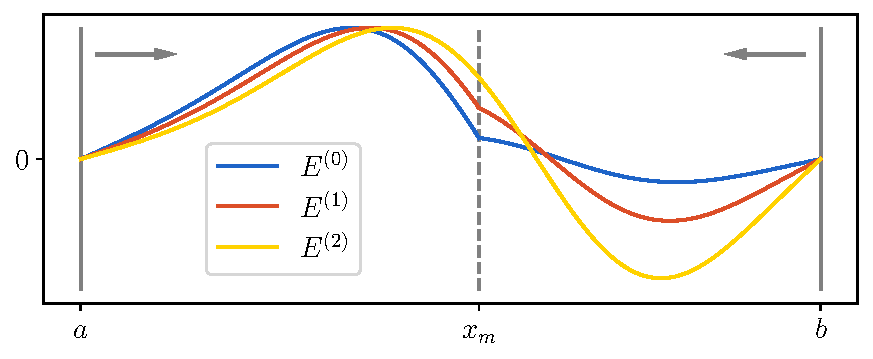
\includegraphics[width=\linewidth]{img/chapter2/shooting_schematic.pdf}
        \caption{Multiple shooting procedures are applied to a Sturm-Liouville equation with homogeneous Dirichlet boundary conditions. $E^{(0)}$ is a possible first eigenvalue guess, $E^{(1)}$ and $E^{(2)}$ are consecutive adjustments. Notice that for $E^{(2)}$ a differentiable function in the matching point $x_m$ is found.}
        \label{fig:c2_shooting_schematic}
    \end{center}
\end{figure}

The main idea of shooting is, when a method for the initial value problem is available, to `guess' a value $\lambda = E$. With this guess, the forward initial value problem is solved from the left side of the domain up to a point $x_m$, and also, a backward initial value problem is solved from the right side to the same point $x_m$. If the forward solution and the backward solution emit a global continuously differentiable solution, then $\lambda = E$ is a valid eigenvalue. If this is not the case, $E$ is adjusted, and the procedure repeats. In figure \ref{fig:c2_shooting_schematic} this is schematically demonstrated.

More concretely, to apply this technique to the Schrödinger equation \eqref{equ:c2_cpm_schrodinger} we again assume $E$ is fixed and convert it to a forward (left) initial value problem:
$$
    -y_\text{L}''(x) + V(x) y_\text{L}(x) = E y_\text{L}(x)
$$
with the starting condition
$$
    y_\text{L}(a) = \beta_a \text{ and } y_\text{L}'(a) = -\alpha_a\text{.}
$$
Analogously, we define a backward (right) initial value problem:
$$
    -y_\text{R}''(x) + V(x) y_\text{R}(x) = E y_\text{R}(x)
$$
with the starting condition
$$
    y_\text{R}(b) = \beta_b \text{ and } y_\text{R}'(b) = -\alpha_b\text{.}
$$

Now, the domain $[x_\text{min}, x_\text{max}]$ is partitioned in $K$ intervals. The $i^\text{th}$ interval can be written as $I_i = [x_{i-1}, x_{i}]$, with $a = x_0, x_1, \dots, x_{K-1}, x_{K} = b$ the grid points. One of these grid points can now be chosen as the matching point $x_m$. Note that numerically it is a little easier if this matching point is not in the exact center of the domain. If the potential happens to be zero, the eigenfunctions will have roots in this center. And, if the matching points coincide with a root, care has to be taken to determine the scaling of the left and right solutions.

Generically we can write such an interval as $I = [X, X+h]$. On $I$, the solution $y$ can now be expressed as:
\begin{equation}
    \begin{pmatrix}y(X+\delta) \\ y'(X+\delta)\end{pmatrix}
    = \begin{pmatrix} u(\delta) & v(\delta) \\ u'(\delta) & v'(\delta) \end{pmatrix} \begin{pmatrix} y(X) \\ y'(X) \end{pmatrix} \,, \qquad %\text{ with } 
    0 \leq \delta \leq h \,. \label{equ:c2_cpm_propmatrix}
\end{equation}

The functions $u(\delta)$ and $v(\delta)$ are the propagators from theorem \ref{the:c2_perturbation_terms} with the initial conditions $u(0) = 1, u'(0)=0$ and
$v(0) = 0, v'(0)=1$. This matrix is called the one-step propagation matrix:
\begin{equation}\label{equ:c2_propagation_matrix}
    \vb{P}(\delta) = \begin{pmatrix} u(\delta) & v(\delta) \\ u'(\delta) & v'(\delta) \end{pmatrix}\text{.}
\end{equation}
To execute backward propagation, its inverse can be determined. In $\delta = 0$, due to the initial conditions, the determinant of $\vb{P}(0)$ is one. To determine the determinant throughout the domain we compute its derivative with respect to $\delta$.
\begin{align*}
    \dv[]{\det\vb{P}}{\delta} & = \left(u(\delta) v'(\delta) - u'(\delta) v(\delta)\right)' \\
                              & = u'' v + u'v' - u''v - u'v'                                \\
                              & =(V(X+\delta) - E) u v - u (V(X+\delta) - E) v              \\
                              & =0
\end{align*}

This implies that $\det\vb{P}(\delta) = 1$, for each $0\leq \delta\leq h$. Which allows us to write down $\vb{P}^{-1}(\delta)$:
$$
    \vb{P}^{-1}(\delta) = \begin{pmatrix} v'(\delta) & -v(\delta) \\ -u'(\delta) & u(\delta) \end{pmatrix}\text{.}
$$
This matrix can now be used for the backward initial value problem.

If we compute on each interval left of $x_m$ the matrix $\vb{P}(h)$ and on each interval to the right of $x_m$ we compute $\vb{P}^{-1}(h)$, then the solution of $y_\text{L}(x_m)$, $y_\text{L}'(x_m)$ and $y_\text{R}(x_m)$, $y_\text{R}'(x_m)$ can be determined.

To know if the guess for $E$ was correct we need to find a scaling of $y_\text{L}$ and $y_\text{R}$ such that $y_\text{L}(x_m) = y_\text{R}(x_m)$ and $y_\text{L}'(x_m) = y_\text{R}'(x_m)$. This can be expressed as a matching error function:
$$
    e(E) = y_\text{L}(x_m) y_\text{R}'(x_m) - y_\text{L}'(x_m) y_\text{R}(x_m)\text{.}
$$

The goal now is to find all zero-values of this function. For this, we use the Newton-Raphson method. Computing the derivative $\dv[]{e(E)}{E}$ is far from trivial. But in theorem \ref{the:c2_perturbation_terms} we see the dependence on $E$ of each $u(h)$ and $v(h)$ through $Z(\delta) = \eta_i\left((V(x) - E)\delta^2\right)$. In theorem \ref{the:c2_eta_functions} we provided the needed derivatives. These can be used to also compute the derivative of $e(E)$ with respect to $E$. This allows for fast convergence to true eigenvalues $E \to \lambda$, for which $e(\lambda) = 0$.

\begin{figure}
    \begin{center}
        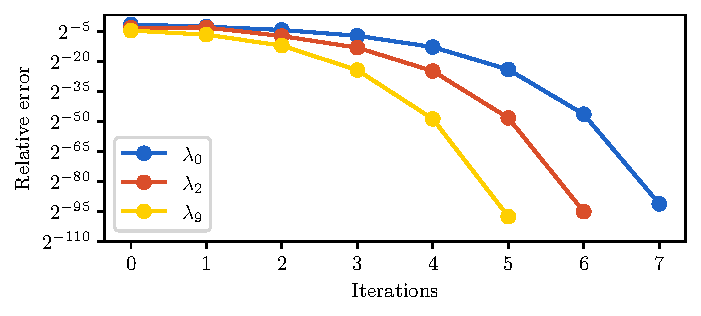
\includegraphics[width=\textwidth]{img/chapter2/prufer/shooting_convergence_float128.pdf}
    \end{center}
    \caption{Using shooting, the relative error of estimates for different eigenvalues of \eqref{ref:equ_shooting_paine} is plotted with respect to the number of iterations of the Newton-Raphson procedure.}\label{fig:c2_shooting_convergence}
\end{figure}

As an example we consider one of Paine's problems from \cite{paine_correction_1981}. On the domain $[0, \pi]$, we will solve the Schrödinger equation
\begin{equation}\label{ref:equ_shooting_paine}
    -y''(x) + e^x y(x) = \lambda y(x)
\end{equation}
with homogeneous Dirichlet boundary conditions. In \cite{paine_correction_1981}, the eigenvalues are reported with five decimal digits, \pyslise{} agrees for all provided digits. The first twelve eigenvalues with 24 fractional digits are reported here.
\begin{center}
    \begin{tabular}{n{2}{24}n{3}{24}}
        4.896669379967691490474902  & 56.181594022847580296684220  \\
        10.045189893253741994613494 & 71.152997537057822221278311  \\
        16.019267250492220805222091 & 88.132119191546181466153432  \\
        23.266270940022341911164117 & 107.116676138267797713195715 \\
        32.263707045804466735963540 & 128.105021273333317509823750 \\
        43.220019640534137263517478 & 151.096043745596921632322296
    \end{tabular}
\end{center}

In figure \ref{fig:c2_shooting_convergence}, the convergence of the Newton-Raphson procedure is visualized. We have started with the guesses $3$, $18$ and $102$ to find the respective eigenvalues $\lambda_0 \approx \numprint{4.896669}$, $\lambda_2 \approx \numprint{16.019267}$  and $\lambda_9 \approx \numprint{107.116676}$. From the graphs we see that the convergence is definitely faster than linear. After at most merely six iteration steps we have reached the maximal precision of the \texttt{double} datatype ($10^{-16} \approx 2^{-53}$) and with one more iteration we reach close to the maximal precision of the \texttt{float128} datatype ($10^{-34} \approx 2^{-112}$). In a table, it becomes clear that the convergence has a quadratic behavior. Here the relative errors are tabulated from the second iteration onward.

\begin{center}
    \begin{tabular}{r|n{1}{0}n{1}{0}n{1}{0}n{1}{0}n{1}{0}n{1}{0}}
                                     & {2}  & {3}  & {4}   & {5}   & {6}   & {7}   \\
        \hline
        \rule{0pt}{2.6ex}$\lambda_0$ & 6e-2 & 8e-3 & 2e-4  & 6e-8  & 1e-14 & 4e-28 \\
        $\lambda_2$                  & 7e-3 & 1e-4 & 4e-8  & 3e-15 & 2e-29 &       \\
        $\lambda_9$                  & 3e-4 & 5e-8 & 2e-15 & 4e-30 &       &       \\
    \end{tabular}
\end{center}

Note that this example has been performed in quadruple floating point precision. This is only possible because of our improvements from section \ref{sec:c2_generalizing_scalar}.


There still remains one problem: how do we ensure that we have found \emph{all} eigenvalues?

For this we remember theorem \ref{the:c2_kth_eigen_k_roots}. To know the index of the eigenvalue we can `simply' count the number of roots the corresponding eigenfunction has. In practice this is quite hard, especially for highly oscillatory eigenfunctions. For these it is very easy to miss a few roots.

To combat this issue and to provide a reliable way to count the roots of even highly oscillatory eigenfunctions Prüfer's scaled transformation can be used \cite{pruefer_neue_1926}.

\begin{theorem}[Prüfer 1926]\label{the:c2_prufer_transformation}
    For a fixed value $E$ define $\theta(x)$ and $\rho(x)$ as the continuous functions which satisfy
    \begin{equation}\label{equ:c2_prufer_theta}
        y(x) = \frac{1}{\sqrt{S(x)}} \rho(x) \sin(\theta(x)) \quad\text{ and }\quad p(x)y'(x) = \sqrt{S(x)} \rho(x) \cos(\theta(x))
    \end{equation}
    with $\theta(a) = -\atan\frac{S(a)\beta_a}{\alpha_a}$ and $S(x)$ a strictly positive scaling function and to ensure numerical stability.
    Here $y(x)$ is a solution of the Sturm-Liouville equation
    $$
        -\dv[]{p(x)y'(x)}{x} + q(x) y(x) = E w(x) y(x)
    $$
    on the interval $[a, b]$ with boundary conditions $\alpha_a y(a) + \beta_a p(a) y(a) = 0$ and $\alpha_b y(b) + \beta_b p(b) y(b) = 0$.

    Define $k$ to be
    $$
        k = \frac{1}{\pi}\left(\theta(b) + \atan\frac{S(b)\beta_b}{\alpha_a}\right) \text{.}
    $$
    If $k$ is an integer, then $y(x)$ has $k$ roots and satisfies the Sturm-Liouville problem. In other words, $\lambda_k = E$ is the $k^\text{th}$ eigenvalue.

    $y(x)$ has $k$ roots in $[a, b]$ and $E$ is the $k^\text{th}$ eigenvalue.
\end{theorem}

Imposing that $\theta(x)$ and $\rho(x)$ as continuous functions ensures that \eqref{equ:c2_prufer_theta} uniquely defines these functions. Without using continuity, $\theta(x)$ can be calculated as
\begin{equation}\label{equ:c2_prufer_theta_up_to_pi}
    \theta(x) = \atan\frac{S(x)y(x)}{y'(x)} + j\pi
\end{equation}
with $j$ integer. If $\theta(x)$ has to be continuous we can uniquely determine which value $j$ should be. To compute $\theta(x)$ efficiently and reliably we have to define it with the differential equation:
\begin{equation}\label{equ:c2_prufer_theta_ode}
    \theta' = \frac{S}{p} \cos^2(\theta) + \frac{Ew - q}{S}\sin^2\theta + \frac{S'}{S}\sin(\theta)\cos(\theta)\text{.}
\end{equation}

\begin{figure}
    \begin{center}
        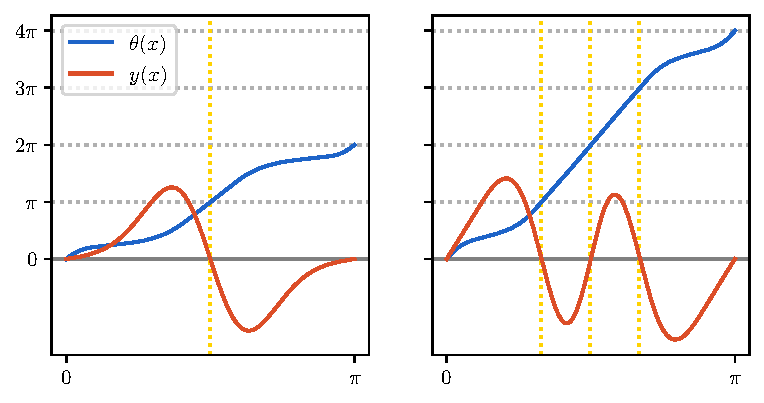
\includegraphics[width=\textwidth]{img/chapter2/prufer/prufer_curves.pdf}
    \end{center}
    \caption{Eigenfunction $y_1(x)$ and $y_3(x)$ for the Mathieu problem with $q = 10$ from section \ref{sec:c2_numerical_experiments_mathieu}. The scaled Prüfer angle $\theta(x)$ is plotted as well.}\label{fig:c2_prufer_curves}
\end{figure}

In the implementation while propagating solutions with equation \eqref{equ:c2_cpm_propmatrix} we also solve \eqref{equ:c2_prufer_theta_ode}. Luckily, this second ordinary differential equation does not need to be solved accurately, because the very accurate value of $y$ can be used to compute $\theta(x)$ with equation \eqref{equ:c2_prufer_theta_up_to_pi} up to a multiple of $\pi$. The value computed with \eqref{equ:c2_prufer_theta_ode} can then be rounded to the nearest value found with \eqref{equ:c2_prufer_theta_up_to_pi}.

Much has been written \todo{Some more sources} about the best choices for the scaling function $S(x)$, in our implementation we follow Matslise as written in \cite{ledoux_study_2007}.

As an illustration of this scaled Prüfer transformation with equation \eqref{equ:c2_prufer_theta_ode} we present figure \ref{fig:c2_prufer_curves}. Here two eigenfunctions from the Mathieu problem from section \ref{sec:c2_numerical_experiments_mathieu} with $q=10$ are plotted. The scaled Prüfer angles can be seen in blue. Notice that the Prüfer angle crosses a multiple of $\pi$ if and only if the corresponding $x$ value is a zero of $y(x)$. The final value of $\theta(b) / \pi - 1$ on the right most point of the domain tells us the index of the relevant eigenvalue.

\section{Matslise 3.0}\label{sec:c2_matslise3}

In the previous section we have studied the background of constant perturbation methods. From here on out we develop our additions to these well-established methods. Some of these results were published in \cite{baeyens_fast_2020}, particularly this section \ref{sec:c2_matslise3} and some numerical experiments: \ref{sec:c2_numerical_experiments_mathieu}, \ref{sec:c2_numerical_experiments_coffey_evans} and \ref{sec:c2_numerical_experiments_hydrogen}. The other numerical experiments from \ref{sec:c2_numerical_experiments} take a closer look at our improvements since \cite{baeyens_fast_2020} to the algorithm. In section \ref{sec:c2_periodic}, we present how the constant perturbation method can be used to solve periodic boundary conditions as well. And, later on in section \ref{sec:c2_the_implementation} we take a deep dive into how our new efficient implementation is build.

In 2005 the first version of Matslise \cite{ledoux_matslise_2005}, A \matlab{} package for solving Sturm-Liouville problems (SLP), was published. This program was a modern take on the successful constant perturbation (CP) method based code SLCPM12 \cite{ixaru_slcpm12_1999}. It was the first implementation of CP methods in the user-friendly and then modern numerical computing environment \matlab{}. Up to that point most, if not all, of these programs for solving Sturm-Liouville problems (SLCPM12, SLEIGN, SLEDGE, \dots) \cite{ixaru_slcpm12_1999,bailey_sleign2_2001,eastham_sledge_1996} were written in \fortran{}.

Matslise provided a graphical user interface that made it easy for all researchers to effectively solve the Sturm-Liouville equation without any knowledge of a particular programming language. Before it's release, if one wanted to solve a particular SLP, sufficient knowledge of \fortran{} was needed to implement the problem at hand.

In 2016 a new version, \matslise{2}\cite{ledoux_matslise_2016}, was released. In this whole new version of Matslise generalized CP methods for SLP were implemented. These new methods enabled one to solve the SLP without explicitly transforming the equation to the Liouville normal form. Avoiding this normalization also made it possible to solve new types of Sturm-Liouville problems. As of this writing \matslise{2} has been downloaded over a thousand times, according to SourceForge. This number proves the need of current research to solve the SLP equation.

As the original Matslise modernized the implementation of SLCPM12, the need to remodernize this proven package has become apparent in our attempt to use, following the ideas of Ixaru in \cite{ixaru_new_2010}, the Matslise routines to solve the multidimensional Schrödinger equation. This approach requires the fast and accurate computation of both the eigenvalues and the corresponding eigenfunctions of several 1D Schrödinger-problems. The \matslise{2} version however mainly focuses on the fast and accurate computation of eigenvalues and the graphical representation of the eigenfunction. In \matslise{2} the eigenfunctions can be computed quite accurate and fast, but only in a limited set of points (depending on the partition of the integration interval). The accurate computation of the eigenfunction over the whole integration interval however is time-consuming in the implementation of \matslise{2}.

In fact, this illustrates that \matslise{2} has not been built as a library of functions, but as a set of functions around a central GUI to solve SLP (and Schrödinger problems in particular). Several other features illustrate this, such as the algorithm that is used to detect whether a given problem is singular and the automatic computation of the error estimates for the eigenvalues. The algorithms are very useful for solving a particular SLP, but valuable computation time is lost if this detection or the error estimation is not needed.

These challenges were the main motivator for a more efficient implementation of Matslise. We have considered different ways to optimize Matslise, keeping in mind its main features, in particular its user-friendliness, one of the main reason for the development of the first version of Matslise.

In this section we give an overview of our theoretical advancements \cite{baeyens_fast_2020} in building a very efficient implementation of the constant perturbation method. Later on, in section \ref{sec:c2_numerical_experiments} we will perform some numerical experiments and some run-time analysis. In section \ref{sec:c2_the_implementation} we will take the time to take a look at the challenges we faced and the choices we made when building our new implementation.

\subsection{The CP method for Schrödinger problems}\label{the-method}

CP methods have already been described extensively, see e.g.\ \cite{ixaru_numerical_1984,ixaru_cp_1998,ixaru_cp_2000,ledoux_cp_2004}. The main bricks for the CP method and related $\eta$-functions were laid in \cite{ixaru_numerical_1984}. We present a short overview for the Schrödinger equation in particular; for a more in depth explanation see the previously mentioned references.

The one dimensional time independent Schrödinger equation is of the form
$$
    -y''(x) + V(x)y(x) = \lambda y(x)\text{.}
$$
The function $V(x)$ is called the potential function. This eigenvalue problem is mostly considered as a boundary value problem on the interval $[a, b]$. We further assume that the boundary conditions are homogeneous Robin conditions, i.e.~they can be expressed as
$$
    \alpha_a y(a) + \beta_a y'(a) = 0 \text{ and } \alpha_b y(b) + \beta_b y'(b) = 0\text{,}
$$
with not both $\alpha_a$ and $\beta_a$ zero (analogous for $\alpha_b$ and $\beta_b$).


\subsection{New formulae for the computation of the eigenfunctions}\label{sec:c2_cp_in_delta}

In section \ref{the-method} we have provided an overview of the CP method to solve the one-dimensional Schrödinger equation. This method can be summarized in the following steps:
\begin{itemize}
    \item Split the domain $[a, b]$ in intervals $(a=x_0, x_1, x_2, \dots, x_k, \dots, x_n = b)$.
    \item For each interval $k$ write $X = x_{k-1}$ and $h = x_k - x_{k-1}$. \begin{itemize}
              \item Construct propagators $u(\delta)$ and $v(\delta)$ for $\delta \in [0, h]$, according to the formulae from theorem \ref{the:c2_perturbation_terms}.
              \item A solution $y(x)$ can be calculated on the $k^\text{th}$ interval if $y(X)$ is known:
                    \begin{align*}
                        y(X+\delta)  & = u(\delta)y(X) + v(\delta)y'(X)   \\
                        y'(X+\delta) & = u'(\delta)y(X) + v'(\delta)y'(X)
                    \end{align*}
          \end{itemize}
    \item Employ multiple shooting to find solutions to the boundary value problem.
\end{itemize}

Up to now the perturbation terms for $u(\delta)$ and $v(\delta)$ given in Theorem \ref{the:c2_perturbation_terms} were only calculated and implemented with $\delta = h$. In that case, one not only obtains superconvergence as formulated in Theorem \ref{the:c2_h_error_estimate}, but there is also a major simplification in symbolic complexity. Nevertheless, for higher orders even these 'simplified' formulae are daunting to work with.

For the efficient calculation of eigenfunctions in arbitrary points of the domain it would however be beneficial if the propagation terms were also implemented in function of $\delta$. To prove the corresponding mathematical results, we reformulate the expressions of the propagators in terms of $\theta=\delta/h$.

Functions of $\theta$ will be denoted with a bar, like $\bar{C}(\theta) = C(\theta h)= C(\delta)$ and $\bar{u}_{q}(\theta) = {u}_{q}(\theta h) =u_{q}(\delta)$. Again $\bar{p}$ generically denotes  the functions $\bar{u}$ or $\bar{v}$. The CP-correction terms are now given by:
\begin{align}
     & \bar{p}_q(\theta) = \sum_{i=-1}^\infty h^{2i+1}\theta^{2i+1} \bar{C}^{(q)}_i(\theta) \eta_{i}(Z(h\theta))
    \intertext{with derivative:}
     & \begin{aligned}
        \bar{p}_q'(\theta) & = \sum_{i=-1}^\infty \left(\bar{C}_{i}^{(q)\prime}(\theta) + h^2 \theta \bar{C}_{i+1}^{(q)}(\theta)\right) h^{2i + 1} \theta^{2i + 1}\eta_{i}(Z) \\
                           & \quad \quad + \frac{\bar{C}_{-1}^{(q)}(\theta)}{\theta^2 h}\left(\eta_{-1}(Z)+Z\eta_{0}(Z)\right) \text{.}
    \end{aligned}
\end{align}
The functions $\bar{C}^{(q)}_i$ satisfy the following recursive relation:
\begin{align}
    \bar{C}_i^{(q)}(\theta)    & = \frac{\theta^{-i}}{2} \int_0^\theta \sigma^{i-1} \left(
    \bar{C}_{i-1}^{(q-1)}(\sigma) \Delta V(X+h\sigma) -  h^{-2} \bar{C}_{i-1}^{(q)\prime\prime}(\sigma)
    \right)\dd\sigma \nonumber                                                             \\
    \bar{C}_{i}^{(0)}(\theta)  & = \begin{cases}
        h\theta & \text{if $p = u$ and $i = -1$} \\
        1       & \text{if $p = v$ and $i = 0$}  \\
        0       & \text{otherwise}
    \end{cases}                              \\
    \bar{C}_{-1}^{(q)}(\theta) & = 0 \quad \text{if $q > 0$}\,.\nonumber
\end{align}


Denoting $\bar{y}(\theta) = y(X+\theta\,h)$, the propagation relation (\ref{equ:c2_cpm_propmatrix}) can be rewritten

\begin{equation}
    \begin{pmatrix}\bar{y}(\theta)\\ \bar{y}'(\theta)\end{pmatrix}
    = \begin{pmatrix} \bar{u}(\theta) & \bar{v}(\theta)/h \\ \bar{u}'(\theta) & \bar{v}'(\theta)/h \end{pmatrix} \begin{pmatrix} \bar{y}(0) \\ \bar{y}'(0) \end{pmatrix} \,, \qquad %\text{ with } 
    0 \leq \theta \leq 1 \,. \label{equ:c2_cpm_propmatrix2}
\end{equation}

\begin{theorem}[Baeyens and Van Daele 2021]\label{the:c2_delta_formulae}
    Assume, for $h$ sufficiently small, that an approximation of the propagation matrix % in $\theta = \frac{\delta}{h} \in [0, 1]$
    $$
        \begin{pmatrix}
            \bar{u}(\theta)  & \bar{v}(\theta)/h  \\
            \bar{u}'(\theta) & \bar{v}'(\theta)/h
        \end{pmatrix}
    $$
    is desired to be accurate to at least $\mathcal{O}(h^r)$. % , i.e. the error has to be a multiple of $h^{r+1}$.
    Then the number of correction terms $Q$ has to be at least $\lfloor\frac{r}{3} \rfloor$
    and $V$ can be approximated by a polynomial of degree $N=r-2$.

\end{theorem}
\begin{proof}
    This theorem is heavily inspired by \cite{ixaru_cp_1998}. There an error estimate is calculated and Theorem~\ref{the:c2_perturbation_terms} and Theorem~\ref{the:c2_h_error_estimate} are proved. These proofs give a useful framework for providing a result for the $\delta$-dependent formulae.

    First we show by induction on $q$ and $i$ that $\bar{C}_{i}^{(q)}$ is a polynomial in both $\theta$ and $h$ whereby for each term the power in $h$ is not smaller than the power in $\theta$. This indeed holds for all $i$ when $q=0$ and for all $q$ when $i=-1$. Assuming that this also holds for $\bar{C}_{i-1}^{(q-1)}$ and $\bar{C}_{i}^{(q-1)}$, we will show that it also holds for $\bar{C}_{i}^{(q)}$. Indeed, $h^{-2}\bar{C}_{i-1}^{(q)\prime\prime}(\sigma)$ is a polynomial satisfying the same property and
    $$
        \sigma^{i-1} \left(
        \bar{C}_{i-1}^{(q-1)}(\sigma) \Delta V(X+h\sigma) - h^{-2} \bar{C}_{i-1}^{(q)\prime\prime}(\sigma)
        \right)
    $$
    is a polynomial of degree at least $i-1$ in $\sigma$. After integrating w.r.t.\ $\sigma$ between $0$ and $\theta$ and multiplying by $\theta^{-i}$, it follows that $\bar{C}_{i}^{(q)}(\theta)$ is a new polynomial in which no terms have gained factors in $\theta$ nor has any lost factors of $h$, i.e.\ the result is a polynomial in $\theta$ and $h$ with in each term at least as many factors in $h$ as in $\theta$.

    Further, one notices that if both $\bar{C}_{i-1}^{(q-1)}$ and $\bar{C}_{i-1}^{(q)}$ are zero, so is $\bar{C}_{i}^{(q)}$. With the given conditions, it is easy to verify that
    $$
        \bar{C}_{i}^{(q)}(\theta) =  \begin{cases}
            \text{$0$ for $i <q -1$,} & \text{if $\bar{p} = \bar{u}$,} \\
            \text{$0$ for $i <q$,}    & \text{if $\bar{p} = \bar{v}$.}
        \end{cases}
    $$
    In case $\bar{C}_{i}^{(q)}(\theta)$ is not zero, we investigate the common degree in $h$ of all its terms. Let us denote this common degree in $d_h(\bar{C}_{i}^{(q)})$.  Since $\Delta V$ does not contain a constant term, $d_h\left(\bar{C}_{q-1}^{(q)}\right) = d_h\left(\bar{C}_{q-2}^{(q-1)}\right)+1$.
    On the other hand $d_h\left(\bar{C}_{i}^{(q)}\right)=d_h\left(\bar{C}_{i-1}^{(q)}\right)-2$.

    For $\bar{p}=\bar{u}$, we have $d_h\left(\bar{C}_{-1}^{(0)}\right)=1$ such that $d_h\left(\bar{C}_{q-1}^{(q)}\right)=q+1$ and $d_h\left(\bar{C}_{i}^{(q)}\right) = q+1-2(i-(q-1))=3q-2i-1$ for $i \geq q-1$.

    For $\bar{p}=\bar{v}$, we similarly have $d_h\left(\bar{C}_{0}^{(0)}\right)=0$ such that $d_h\left(\bar{C}_{q}^{(q)}\right)=q$ and $d_h\left(\bar{C}_{i}^{(q)}\right) = q-2(i-q)=3q-2i$ for $i \geq q$.
    %For $\bar{p} = \bar{v}$ and $d_h(\bar{C}_{i}^{(q)})=3q-2i$ for $\bar{p} = \bar{v}$.

    Combining these results and assuming all $\eta_i(Z(h\theta))$ are bounded we get:
    % {\color{red}
    \begin{align*}
        \bar{u}_{q}(\theta)   & =  \sum_{i=q-1} h^{2i+1} \theta^{2i+1} \bar{C}^{(q)}_i(\theta) \eta_{i}(Z(h\theta)) = \mathcal{O}(h^{3q})     \\
        \bar{v}_{q}(\theta)/h & = h^{-1} \sum_{i=q} h^{2i+1} \theta^{2i+1} \bar{C}^{(q)}_i(\theta) \eta_{i}(Z(h\theta)) = \mathcal{O}(h^{3q})
    \end{align*}
    % }

    Using the expression for the derivative $\bar{p}'_{q}(\theta)$, one can similarly prove

    \begin{align*}
        \bar{u}'_{q}(\theta)   & =  \mathcal{O}(h^{3q}) \\
        \bar{v}'_{q}(\theta)/h & = \mathcal{O}(h^{3q})
    \end{align*}

    We can thus indeed conclude that, in order to be accurate up to order $r$ in $h$, we need to consider all terms $\bar{p}_q(\theta)$, $q=0,1,2,\ldots$ for which $3q \leq r$, i.e. $Q= \lfloor \frac{r}{3} \rfloor$.

    Next we determine the minimal value of $N$, the degree of the polynomial approximation $V^{N}(x)$ of $V$, to obtain a given accuracy.

    We first consider the case $p=u$, and we will show that for $i \geq q-1$ each term in $\bar{C}_i^{(q)}$ contains a factor of the form $ V_{j_1} V_{j_2} \cdots V_{j_q} h^{j_1+j_2+\ldots+j_q+1 - 2 (i-(q-1))}$. For $\bar{C}_0^{(1)}$ all terms indeed contain an expression $V_j h^{j+1}$ and by induction we find for $i>0$, since $\bar{C}_i^{(0)}(\theta)=0$, that all terms in $\bar{C}_i^{(1)}$ have a factor of the form $V_j h^{j+1-2i}$. Assuming this results holds for all $\bar{C}_i^{(q-1)}$ with $i\geq q - 1$, one first verifies that the result also holds for $\bar{C}_{q-1}^{(q)}$ and by induction on $i$,  also for $\bar{C}_{i}^{(q)}$ with $i>q-1$.

    This property of $\bar{C}_i^{(q)}$ can now be used to determine the lowest degree $N$ that leads to the $\mathcal{O}(h^r)$ approximation. Since $\bar{C}_i^{(q)}$ is multiplied with $h^{2i+1}$, it follows that  $\bar{u}_q(\theta)$ contains terms with factors $ V_{j_1} V_{j_2} \cdots V_{j_q} h^{j_1+j_2+\ldots+j_q+ 2 q }$ with $1 \leq j_k \leq N$, $k=1,\ldots, q$. For $q=1$ we have $V_{j} h^{j+2} $, which can only be discarded when $j>r-2$. Thus choosing $N=r-2$ will only discard these terms. The choice $N=r-2$ is also sufficient when $q>1$. We can thus conclude that, in order to obtain accuracy up to order $h^r$ in $\bar{u}(\theta)$ it suffices to take $N=r-2$.

    For $p=v$, one similarly shows that all terms in $\bar{C}_i^{(q)}$ contain expressions of the form $ V_{j_1} V_{j_2} \cdots V_{j_q} h^{j_1+j_2+\ldots+j_q - 2 (i-q)}$ for $i \geq q$. Then $\bar{v}_q(\theta)/h$ contains terms with factors $ V_{j_1} V_{j_2} \cdots V_{j_q} h^{j_1+j_2+\ldots+j_q+ 2 q}$ and all necessary terms will be generated when $N = r-2$.

    For the expressions of the derivatives $\bar{u}'(\theta)$ and $\bar{v}'(\theta)/h$ no extra term is needed. So in summary, $\Delta V$ can be truncated to a degree of $r - 2$.

\end{proof}

To illustrate this theorem we give the first terms in the error $\Delta \bar{p}_{(Q)} = \bar{p}(\theta) - \displaystyle\sum_{i=0}^{Q} \bar{p}_{i}(\theta)$  of the propagation formulae.

\begin{align*}
    \intertext{Zero correction terms}
    \Delta \bar{u}_{(Q=0)}    & = h^{3}\left(\left(\frac{1}{2} \theta^{3} - \frac{1}{2} \theta^{2}\right) V_{1} \eta_{0} -\frac{1}{2} \theta^{3} V_{1} \eta_{1}\right) + \mathcal{O}(h^{4})                                                                              \\
    \Delta \bar{v}_{(Q=0)}/h  & = h^{3}\left(\left(\frac{1}{2} \theta^{4} - \frac{1}{2} \theta^{3}\right) V_{1} \eta_{1}\right) + \mathcal{O}(h^{4})                                                                                                                     \\
    \Delta \bar{u}'_{(Q=0)}   & = h^{3}\left(\left(\frac{1}{2} \theta^{2} - \frac{1}{2} \theta\right) V_{1} \eta_{-1} + \left(\frac{1}{2} \theta^{2} - \frac{1}{2} \theta\right) V_{1} \eta_{0}\right) + \mathcal{O}(h^{4})                                              \\
    \Delta \bar{v}'_{(Q=0)}/h & = h^{3}\left(\left(\frac{1}{2} \theta^{3} - \frac{1}{2} \theta^{2}\right) V_{1} \eta_{0} + \frac{1}{2} \theta^{3} V_{1} \eta_{1}\right) + \mathcal{O}(h^{4})                                                                             \\
    \intertext{One correction term}
    \Delta \bar{u}_{(Q=1)}    & = h^{6}\left(\left(\frac{1}{8} \theta^{6} - \frac{1}{4} \theta^{5} + \frac{1}{8} \theta^{4}\right) V_{1}^{2} \eta_{1} + \left(-\frac{7}{24} \theta^{6} + \frac{1}{4} \theta^{5}\right) V_{1}^{2} \eta_{2}\right)                         \\
                              & \qquad\qquad + \mathcal{O}(h^{7})                                                                                                                                                                                                        \\
    \Delta\bar{v}_{(Q=1)}/h   & = h^{6}\left(\left(\frac{1}{8} \theta^{7} - \frac{1}{4} \theta^{6} + \frac{1}{8} \theta^{5}\right) V_{1}^{2} \eta_{2} -\frac{1}{24} \theta^{7} V_{1}^{2} \eta_{3}\right) + \mathcal{O}(h^{7})                                            \\
    \Delta \bar{u}'_{(Q=1)}   & = h^{6}\left(\left(\frac{1}{8} \theta^{5} - \frac{1}{4} \theta^{4} + \frac{1}{8} \theta^{3}\right) V_{1}^{2} \eta_{0} + \left(\frac{1}{12} \theta^{5} - \frac{1}{4} \theta^{4} + \frac{1}{8} \theta^{3}\right) V_{1}^{2} \eta_{1}\right. \\
                              & \qquad\qquad \left. -\frac{7}{24} \theta^{5} V_{1}^{2} \eta_{2}\right) + \mathcal{O}(h^{7})                                                                                                                                              \\
    \Delta \bar{v}'_{(Q=1)}/h & = h^{6}\left(\left(\frac{1}{8} \theta^{6} - \frac{1}{4} \theta^{5} + \frac{1}{8} \theta^{4}\right) V_{1}^{2} \eta_{1} + \left(\frac{5}{24} \theta^{6} - \frac{1}{4} \theta^{5}\right) V_{1}^{2} \eta_{2}\right) + \mathcal{O}(h^{7})     \\
    \intertext{Two correction terms}
    \Delta \bar{u}_{(Q=2)}    & = h^{9}\left(\left(\frac{1}{48} \theta^{9} - \frac{1}{16} \theta^{8} + \frac{1}{16} \theta^{7} - \frac{1}{48} \theta^{6}\right) V_{1}^{3} \eta_{2} \right.                                                                               \\
                              & \qquad\qquad \left.
    + \left(-\frac{1}{12} \theta^{9} + \frac{7}{48} \theta^{8} - \frac{1}{16} \theta^{7}\right) V_{1}^{3} \eta_{3} 											%\right.     \\
    %& \qquad\qquad \left. 
    +\frac{1}{48} \theta^{9} V_{1}^{3} \eta_{4}\right) + \mathcal{O}(h^{10})                                                                                                                                                                                             \\
    \Delta \bar{v}_{(Q=2)}/h  & = h^{9}\left(\left(\frac{1}{48} \theta^{10} - \frac{1}{16} \theta^{9} + \frac{1}{16} \theta^{8} - \frac{1}{48} \theta^{7}\right) V_{1}^{3} \eta_{3} \right.                                                                              \\
                              & \qquad\qquad \left. + \left(-\frac{1}{48} \theta^{10} + \frac{1}{48} \theta^{9}\right) V_{1}^{3} \eta_{4}\right) + \mathcal{O}(h^{10})                                                                                                   \\
    \Delta \bar{u}'_{(Q=2)}   & = h^{9}\left(\left(\frac{1}{48} \theta^{8} - \frac{1}{16} \theta^{7} + \frac{1}{16} \theta^{6} - \frac{1}{48} \theta^{5}\right) V_{1}^{3} \eta_{1} \right.                                                                               \\
                              & \qquad\qquad \left. + \left(-\frac{1}{24} \theta^{7} + \frac{1}{16} \theta^{6} - \frac{1}{48} \theta^{5}\right) V_{1}^{3} \eta_{2} \right.                                                                                               \\
                              & \qquad\qquad \left. + \left(-\frac{7}{48} \theta^{8} + \frac{7}{48} \theta^{7}\right) V_{1}^{3} \eta_{3}\right) + \mathcal{O}(h^{10})                                                                                                    \\
    \Delta \bar{v}'_{(Q=2)}/h & = h^{9}\left(\left(\frac{1}{48} \theta^{9} - \frac{1}{16} \theta^{8} + \frac{1}{16} \theta^{7} - \frac{1}{48} \theta^{6}\right) V_{1}^{3} \eta_{2} + \right.                                                                             \\
                              & \qquad\qquad \left. \left(\frac{1}{24} \theta^{9} - \frac{5}{48} \theta^{8} + \frac{1}{16} \theta^{7}\right) V_{1}^{3} \eta_{3} -\frac{1}{48} \theta^{9} V_{1}^{3} \eta_{4}\right) + \mathcal{O}(h^{10})                                 \\
\end{align*}

%{\color{red}
To illustrate the second part of the theorem, we consider $\Delta \bar{p}_{(N)} = \bar{p}(\theta) - \bar{p}_N(\theta)$  whereby $\bar{p}_N(\theta)$ is obtained from
$\bar{p}(\theta)$ in which $V_i = 0$ if $i > N$.

\begin{align*}
    \intertext{Truncation of $\Delta V$ to degree $0$.}
    2\,\Delta \bar{u}_{(N=0)}          & = h^{3}\left(\left(\theta^{3} - \theta^{2}\right) V_{1} \eta_{0} -\theta^{3} V_{1} \eta_{1}\right) + \mathcal{O}(h^{4})                                                                    \\
    \frac{2}{h}\Delta \bar{v}_{(N=0)}  & = h^{3}\left(\left(\theta^{4} - \theta^{3}\right) V_{1} \eta_{1}\right) + \mathcal{O}(h^{4})                                                                                               \\
    2\,\Delta \bar{u}'_{(N=0)}         & = h^{3}\left(\left(\theta^{2} - \theta\right) V_{1} \eta_{-1} + \left(\theta^{2} - \theta\right) V_{1} \eta_{0}\right) + \mathcal{O}(h^{4})                                                \\
    \frac{2}{h}\Delta \bar{v}'_{(N=0)} & = h^{3}\left(\left(\theta^{3} - \theta^{2}\right) V_{1} \eta_{0} + \theta^{3} V_{1} \eta_{1}\right) + \mathcal{O}(h^{4})                                                                   \\
    \intertext{Truncation of $\Delta V$ to degree $1$.}
    2\,\Delta \bar{u}_{(N=1)}          & = h^{4}\left(\left(2 \theta^{4} - 3 \theta^{3} + \theta^{2}\right) V_{2} \eta_{0} + \left(-3 \theta^{4} + 3 \theta^{3}\right) V_{2} \eta_{1}\right) + \mathcal{O}(h^{5})                   \\
    \frac{2}{h}\Delta \bar{v}_{(N=1)}  & = h^{4}\left(\left(2 \theta^{5} - 3 \theta^{4} + \theta^{3}\right) V_{2} \eta_{1} - \theta^{5} V_{2} \eta_{2}\right) + \mathcal{O}(h^{5})                                                  \\
    2\,\Delta \bar{u}'_{(N=1)}         & = h^{4}\left(\left(2 \theta^{3} - 3 \theta^{2} + \theta\right) V_{2} \eta_{-1} + \left(3 \theta^{3} - 3 \theta^{2} + \theta\right) V_{2} \eta_{0} \right.                                  \\
                                       & \qquad\qquad \left. - 3 \theta^{3} V_{2} \eta_{1}\right) + \mathcal{O}(h^{5})                                                                                                              \\
    \frac{2}{h}\Delta \bar{v}'_{(N=1)} & = h^{4}\left(\left(2 \theta^{4} - 3 \theta^{3} + \theta^{2}\right) V_{2} \eta_{0} + \left(3 \theta^{4} - 3 \theta^{3}\right) V_{2} \eta_{1}\right) + \mathcal{O}(h^{5})                    \\
    \intertext{Truncation of $\Delta V$ to degree $2$.}
    2\,\Delta \bar{u}_{(N=2)}          & = h^{5}\left(\left(5 \theta^{5} - 10 \theta^{4} + 6 \theta^{3} - \theta^{2}\right) V_{3} \eta_{0} + \left(-10 \theta^{5} + 15 \theta^{4} - 6 \theta^{3}\right) V_{3} \eta_{1} \right.      \\
                                       & \qquad\qquad \left.+5 \theta^{5} V_{3} \eta_{2}\right) + \mathcal{O}(h^{6})                                                                                                                \\
    \frac{2}{h}\Delta \bar{v}_{(N=2)}  & = h^{5}\left(\left(5 \theta^{6} - 10 \theta^{5} + 6 \theta^{4} - \theta^{3}\right) V_{3} \eta_{1} + \left(-5 \theta^{6} + 5 \theta^{5}\right) V_{3} \eta_{2}\right) + \mathcal{O}(h^{6})   \\
    2\,\Delta \bar{u}'_{(N=2)}         & = h^{5}\left(\left(5 \theta^{4} - 10 \theta^{3} + 6 \theta^{2} - \theta\right) V_{3} \eta_{-1} + \left(10 \theta^{4} - 15 \theta^{3} + 6 \theta^{2} - \theta\right) V_{3} \eta_{0} \right. \\
                                       & \qquad\qquad \left. + \left(-15 \theta^{4} + 15 \theta^{3}\right) V_{3} \eta_{1}\right) + \mathcal{O}(h^{6})                                                                               \\
    \frac{2}{h}\Delta \bar{v}'_{(N=2)} & = h^{5}\left(\left(5 \theta^{5} - 10 \theta^{4} + 6 \theta^{3} - \theta^{2}\right) V_{3} \eta_{0} + \left(10 \theta^{5} - 15 \theta^{4} + 6 \theta^{3}\right) V_{3} \eta_{1} \right.       \\
                                       & \qquad\qquad \left. -5 \theta^{5} V_{3} \eta_{2}\right) + \mathcal{O}(h^{6})
\end{align*}

Remark that in Theorem~\ref{the:c2_delta_formulae}, in contrast to Theorem~\ref{the:c2_h_error_estimate}, no assumption is made on the size of $Z=\delta^2 (V_0-E)$. In the proof of Theorem~\ref{the:c2_h_error_estimate} this distinction was necessary because error terms were expressed
not only in terms of bounded functions $\eta_i(Z)$ but also in terms of the unbounded argument $Z$, whereas in the proof of
Theorem~\ref{the:c2_delta_formulae} all error terms were expressed in terms of $\eta_i(Z)$. This enables us to give $\mathcal{O}(h^{N+2})$ error estimates for all $Z$. However, for sufficiently large negative $Z(h) \ll 0$ the $\mathcal{O}({h^N}/{\sqrt{E}})$ error estimate given in Theorem~\ref{the:c2_h_error_estimate} is sharper than the one given in Theorem~\ref{the:c2_delta_formulae}. This new result shows that the order $P_{ass}$ for large and negative $Z$ is the same as the order for small values for $Z$, thus $P_0 = P_{ass}$. So from now on we can denote a CP-method as $\text{CPM}\{r\}$, this method will be accurate with order $\mathcal{O}(h^r)$ if $N=r-2$ and $Q=\lfloor \frac{r}{3} \rfloor$. As a demonstration we give the formulae for the fourth order method $\text{CPM}\{4\}$:

\begin{align*}
    2\bar{u}^{(4)}            & = 2 \eta_{-1} + h^{3}\left(\left(\theta^{3} - \theta^{2}\right) V_{1} \eta_{0} -\theta^{3} V_{1} \eta_{1}\right)                                                                                                 \\
                              & \quad\quad + h^{4}\left(\left(2 \theta^{4} - 3 \theta^{3} + \theta^{2}\right) V_{2} \eta_{0} + \left(-3 \theta^{4} + 3 \theta^{3}\right) V_{2} \eta_{1}\right)                                                   \\
    \frac{2}{h}\bar{v}^{(4)}  & = 2 \theta \eta_{0} + h^{3}\left(\left(\theta^{4} - \theta^{3}\right) V_{1} \eta_{1}\right) + h^{4}\left(\left(2 \theta^{5} - 3 \theta^{4} + \theta^{3}\right) V_{2} \eta_{1} - \theta^{5} V_{2} \eta_{2}\right) \\
    2\bar{u'}^{(4)}           & = \frac{2Z}{h\theta} \eta_0 + h^{2}\left(\left(\theta^{2} - \theta\right) V_{1} \eta_{-1} + \left(\theta^{2} - \theta\right) V_{1} \eta_{0}\right)                                                               \\
                              & \quad\quad+ h^{3}\left(\left(2 \theta^{3} - 3 \theta^{2} + \theta\right) V_{2} \eta_{-1} + \left(3 \theta^{3} - 3 \theta^{2} + \theta\right) V_{2} \eta_{0} - 3 \theta^{3} V_{2} \eta_{1}\right)                 \\
    \frac{2}{h}\bar{v'}^{(4)} & = \frac{2}{h} \eta_{-1} + h^{2}\left(\left(\theta^{3} - \theta^{2}\right) V_{1} \eta_{0} + \theta^{3} V_{1} \eta_{1}\right)                                                                                      \\
                              & \quad\quad + h^{3}\left(\left(2 \theta^{4} - 3 \theta^{3} + \theta^{2}\right) V_{2} \eta_{0} + \left(3 \theta^{4} - 3 \theta^{3}\right) V_{2} \eta_{1}\right)                                                    \\
\end{align*}%

Further, Theorem~\ref{the:c2_delta_formulae} also gives more insight in the number of correction terms $Q$ needed to construct higher order methods. In \matslise{2} $\text{CPM}\{18, 16\}$ was constructed with $N=16$ and $Q=11$, Theorem~\ref{the:c2_delta_formulae} shows that all necessary terms can be generated with $Q=6$ correction terms.


\paragraph{Evaluating eigenvalues}
Once an eigenvalue is computed in Matslise or \matslise{2}, the corresponding eigenfunction can be visualized. Since the mesh is coarse, such a visualization can only be achieved if extra function evaluations are available in a sufficient number of points. Neither Matslise nor \matslise{2} were optimized do to so. To visualize the eigenfunction $y_k$ that corresponds to a particular eigenvalue $E_k$, a new, sufficiently fine mesh is constructed, and all necessary computations are carried out once again.

To explain why this approach was chosen in Matslise and \matslise{2}, let us consider the propagation matrix in \eqref{equ:c2_cpm_propmatrix}. From theorem \ref{the:c2_perturbation_terms}, we learn that each matrix element can be expressed as a polynomial in $\delta$, whose coefficients depend
via $Z=(V_0-E) \delta^2$ on the functions $\eta_i$ and $\delta$-dependent polynomials $C_j$ that also contain powers of the step length $h$ and the coefficients $V_n$ computed by (\ref{equ:c2_legendre_V}). To compute the formulae in $\text{CPM}\{18\}$ for instance, we will take a look at the expression for $u(\delta)$:
$$
    u(\delta) = \sum_{i = -1}^6 C_i(\delta) \eta_{i}(\delta)
$$
with $C_i$ a polynomial in $\delta$,
$$
    C_i  = \sum_{j=0}^{16} d_{i, j} \delta^j,
$$
whereby $d_{i, j}$ is a polynomial of degree $16-j$ in $h$ with coefficients in $V_1, \dots, V_{16}$. As an example we give a small taste of what $d_{4, 9}$ looks like:

\begin{eqnarray*}
    d_{4, 9}& =&  h^7 \left (0.03125 \, V_{2}^{4} + 0.40625 \, V_{1} V_{2}^{2} V_{3} + 0.21875 \, V_{1}^{2} V_{3}^{2} + 0.46875 \, V_{1}^{2} V_{2} V_{4} \right. \\
    &  & \qquad + 0.1875 \, V_{1}^{3} V_{5} - 67.8125 \, V_{3}^{2} V_{4} - 74.375 \, V_{2} V_{4}^{2} - 158.375 \, V_{2} V_{3} V_{5}         \\
    &  & \qquad - 196.875 \, V_{1} V_{4} V_{5} - 96.5625 \, V_{2}^{2} V_{6} - 218.875 \, V_{1} V_{3} V_{6} - 275.0 \, V_{1} V_{2} V_{7}     \\
    &  & \qquad - 199.125 \, V_{1}^{2} V_{8} + 159909.75 \, V_{1} V_{11} + 101029.5 \, V_{10} V_{2} + 27184.5 \, V_{6}^{2}                  \\
    &  & \qquad \left.+ 56164.5 \, V_{5} V_{7} + 62181.0 \, V_{4} V_{8} + 74868.75 \, V_{3} V_{9} \right)                                                 \\
    &  & + h^6 (\,\dots)  + \dots
\end{eqnarray*}


Although these coefficients can all be computed analytically, it was far from practical to implement these very long formulae in software. Since one was mainly interested in the computation of the eigenvalues, the matrix elements in the propagation matrix were in fact only implemented for $\delta=h$, in which case the formulae could be significantly simplified, which in turn had a positive impact on the computation speed.

For the applications we have in mind, this approach is too time-consuming. We decided to develop a new algorithm that is able to reuse all the data that was previously calculated. Therefore, we have chosen to implement in Matslise 3.0 a $\delta$-independent higher order method that is combined with a $\delta$-dependent formula of lower order. The higher order method is the $\text{CPM}\{18\}$-formula (i.e.\ $N=16$ and $Q=6$) that was also used in Matslise and \matslise{2}. For our error estimation, a $\delta$-dependent version of $\text{CPM}\{16\}$ is implemented ($N=14$ and $Q=5)$, which also allows the fast and accurate evaluation of the eigenfunctions in arbitrary points. In section \ref{sec:c2_numerical_experiments} we will present some numerical experiments in which eigenfunctions are computed as well.

\section{Periodic \texorpdfstring{\oneD}{1D} time-independent Schrödinger equation}\label{sec:c2_periodic}

In contrast to (separated) Robin boundary conditions, in this section we will study generalized periodic boundary conditions. Assume we are solving a regular Sturm-Liouville equation
\begin{equation}\label{equ:c2_periodic_sturm_liouville}
    -\dv[]{p(x)y'(x)}{x} + q(x)y(x) = \lambda w(x) y(x)
\end{equation}
on a domain $[a, b]$, with generalized periodic boundary conditions:
\begin{equation}\label{equ:c2_periodic_boundary_conditions}
    \begin{pmatrix}
        y(a) \\ p(a)y'(a)
    \end{pmatrix} = \vb{K}\begin{pmatrix}
        y(b) \\ p(b)y'(b)\text{.}
    \end{pmatrix}
\end{equation}

In expression \eqref{equ:c2_periodic_boundary_conditions} is $\vb{K}$ assumed to be a $2 \times 2$ real matrix with determinant $1$\cite{binding_prufer_2013}. If $\vb{K} = \vb{I}$, these boundary conditions are called \emph{periodic}, and if $\vb{K} = -\vb{I}$ then they are called \emph{antiperiodic}.

In section \ref{sec:c2_slp_properties} we have provided some theorems about regular Sturm-Liouville problems with homogeneous (separated) Robin boundary conditions. From all these theorems, only theorem \ref{the:c2_real_eigenvalues} is also applicable here. All eigenvalues are real, and eigenfunctions can always be scaled to be real as well.

Following section \ref{sec:c2_background} and \ref{sec:c2_matslise3}, due to the Liouville-transformation (from section \ref{sec:c2_liouville_transformation}) it is sufficient to only consider Schrödinger problems with $p(x) = w(x) = 1$.

Because the equation has not changed the idea and computation of a piecewise constant approximation, perturbation terms and a propagation matrix are still valid and valuable. There are just a few related problems. First, what do we propagate? No obvious initial conditions are available. And second, we are still only interested in continuous and continuously differentiable functions, so the idea of a matching error is relevant. But how can we compute the index of an eigenvalue? Without this, it would be difficult to ensure all requested eigenvalues are found.

For this we employ the results from \cite{binding_prufer_2012,binding_prufer_2013} to expand the Prüfer transformation. In theorem \ref{the:c2_prufer_transformation}, the Prüfer-angle function $\theta(x)$ was defined. This definition assumed initial conditions $y(a) = \beta_a$ and $p(a)y(b) = -\alpha_a$. In the periodic case, no such initial conditions are available. Therefore, we define the Prüfer-angle as a function of the initial conditions $y(a) = \sin(\alpha)$ and $p(a)y'(a) = \cos(\alpha)$. For a fixed value of $E$, define $\theta_\alpha(x)$ with the ordinary differential equation \eqref{equ:c2_prufer_theta_ode} and initial conditions
$$
    \theta_\alpha(a) = \atan(S(a) \tan(\alpha))\text{.}
$$

As in theorem \ref{the:c2_prufer_transformation}, it is necessary to consider the difference with the right most boundary conditions. For this we define the unique $\pi$-periodic function $\beta(\alpha)$ with $\beta(0) \in \left]-\pi, 0\right]$ and
$$
    \tan(\beta(\alpha)) = S(b)\frac{k_{11} \sin(\alpha) + k_{12} \cos(\alpha)}{k_{21} \sin(\alpha) + k_{22} \cos(\alpha)}\text{,}
$$
with
$$
    \vb{K} = \begin{pmatrix}
        k_{11} & k_{12} \\ k_{21} & k_{22}
    \end{pmatrix}\text{.}
$$

With this $\beta(\alpha)$, we define
\begin{align}
    \delta_\alpha(E)       & = \theta_\alpha(b) - \beta(\alpha)\text{,} \nonumber                    \\
    m(E)            & = \min_{\alpha \in \RR} \delta_\alpha(E) \nonumber                             \\
    \text{and }M(E) & = \max_{\alpha \in \RR}\delta_\alpha(E)\text{.}\label{equ:c2_periodic_m_and_m}
\end{align}
In these expressions we have made the dependence on $E$ explicit, as $E$ was previously assumed to be fixed.

The following lemma and theorems, with proofs can be found in \cite{binding_prufer_2012} and \cite{binding_prufer_2013a}
\begin{lemma}[Binding and Volkmer 2012]\label{lem:c2_periodic_m_inequality}\hfill
    \begin{itemize}
        \item The functions $m$ and $M$ are continuous and strictly increasing.
        \item For each $E$, we have the inequalities
              $$
                  -\pi < m(E) < M(E) < m(E) + \pi\text{.}
              $$
    \end{itemize}
\end{lemma}

For the following theorems we need to distinguish between if $k_{12} < 0 \lor k_{12} = 0 < k_{11}$ and the opposite. Let us call the former the periodic case, and the latter the antiperiodic case.

\begin{theorem}[Binding and Volkmer 2012]
    For each eigenvalue $\lambda$ of the Sturm-Liouville equation \eqref{equ:c2_periodic_sturm_liouville} subject to generalized periodic boundary conditions, either $m(\lambda) = k\pi$ or $M(\lambda) = k\pi$ with $k$ integer. In the periodic case will $k$ be even, in the antiperiodic case will $k$ be odd.
\end{theorem}

The last theorem gives us a coupling between the function $m(E), M(E)$ and the eigenvalues of the Sturm-Liouville problem. To reliably determine the index of an eigenvalue we also need the inverse theorem.

\begin{theorem}[Binding and Volkmer 2012]\label{the:c2_prufer_periodic_index}
    Define $\lambda_k^{+}$ to be the unique value for which $m(\lambda_k^{+}) = k\pi$ and $\lambda_k^{-}$ to be the unique value such $M(\lambda_k^{-}) = k\pi$. There is no value $\lambda_0^{-}$.
    \begin{itemize}
        \item If $k$ is even (for the periodic case) or odd (for the antiperiodic case), then all values $\lambda^{\pm}_k$ are eigenvalues of the corresponding Sturm-Liouville problem.
        \item There are no other eigenvalues.
        \item $\lambda_k^{+} < \lambda_{k+1}^{-}$ for each $k \geq 0$.
        \item An eigenfunction belonging to $\lambda_k^{\pm}$ has exactly $k$ zeros in the interval $\left[a, b\right]$.
    \end{itemize}
\end{theorem}

This theorem characterizes all eigenvalues of regular Sturm-Liouville problems with periodic boundary conditions. The eigenvalues are countable. They have a lower bound: $\lambda^+_0$ (for the periodic case) and $\lambda^+_1$ (for the antiperiodic case). Furthermore, it is also known that $\lambda^{\pm}_k \to \infty$ if $k \to \infty$.

\begin{figure}
    \begin{center}
        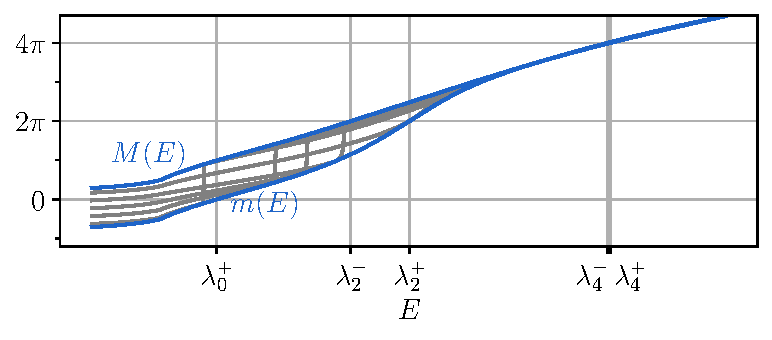
\includegraphics[width=\textwidth]{img/chapter2/prufer/periodic_minmax.pdf}
    \end{center}
    \caption{The scaled Prüfer transformation with different initial conditions for the Schrödinger problem with $q(x) = 3x^2(\pi - x)$ on $[0, \pi]$. The functions $m(E)$ and $M(E)$ from \eqref{equ:c2_periodic_m_and_m} are drawn as well.}\label{fig:c2_periodic_m_and_m}
\end{figure}

As an illustration, we provide figure \ref{fig:c2_periodic_m_and_m}. Here, the expression $\delta_\alpha(E)$ is visualized for varying initial conditions expressed with $\alpha$. All these curves are captured in between $m(E)$ and $M(E)$. The first five eigenvalues of the considered problem are indicated as well. We see that for these values either $m(E)$ or $M(E)$ is an even multiple of $\pi$.

To determine the index of an eigenvalue, theorem \ref{the:c2_prufer_periodic_index} assures us that using the function $m(E)$ and $M(E)$ is sufficient. But efficiently computing these, is no easy task. Since they are defined as extreme values over all possible initial conditions, there is no straightforward way to evaluate them.

We propose to propagate two different initial conditions and use the inequality from lemma \ref{lem:c2_periodic_m_inequality} to estimate $m(E)$ and $M(E)$. More concretely, we apply the propagation matrix from \eqref{equ:c2_propagation_matrix}, not to a single vector, but to a pair of vectors. Both these vectors give rise to two estimates $\delta_1(E)$ and $\delta_2(E)$ of $\delta_\alpha(E)$, without loss of generality we assume $\delta_1 < \delta_2$. From lemma \ref{lem:c2_periodic_m_inequality}, we know
$$
    \delta_2(E) - \pi < m(E) \text{ and } M(E) < \delta_1(E) + \pi \text{.}
$$

Suppose we want to find eigenvalues $\lambda_k^{-}$ and $\lambda_k^{+}$. Now we search for the values $E_1$ and $E_2$ such that
$$
    \delta_1(E_1) + \pi = k \pi \text{ and } \delta_2(E_2) - \pi = k \pi\text{.}
$$

By construction, we know for certain that the interval $[E_1, E_2]$ now contains $\lambda_k^{-}$ and $\lambda_k^{+}$, and it contains no other eigenvalues.

\todo{Still to write: finding the two eigenvalues in the interval $[E_1, E_2]$. First, find the extreme point of the matching error, and then binary search.}

\section{Numerical experiments}\label{sec:c2_numerical_experiments}

As a first numerical experiment, let us verify the order in $h$ and make an estimate for the order in $k$. For this, we use the same problem as in figures \ref{fig:c2_pruess_h_error} and \ref{fig:c2_pruess_k_error}.

\subsection{A first example}

Consider the Schrödinger problem with equation
\begin{equation}\label{equ:c2_matslise_order_test_problem}
    -y'' + 100\cos^2(x)\,y = \lambda y
\end{equation}
on the domain $[a, b] = [0, \pi]$ and homogeneous Dirichlet boundary conditions.

Before jumping into the graphs, we have to note that \matslise{3} has automatic step size selection build in. This allows the algorithm to generate its own piecewise approximation of the potential. But, this also implies that a user is not directly able to control the number of subintervals used, which makes generating a figure like \ref{fig:c2_pruess_k_error} or \ref{fig:c2_pruess_h_error} more difficult.

\begin{figure}
    \begin{center}
        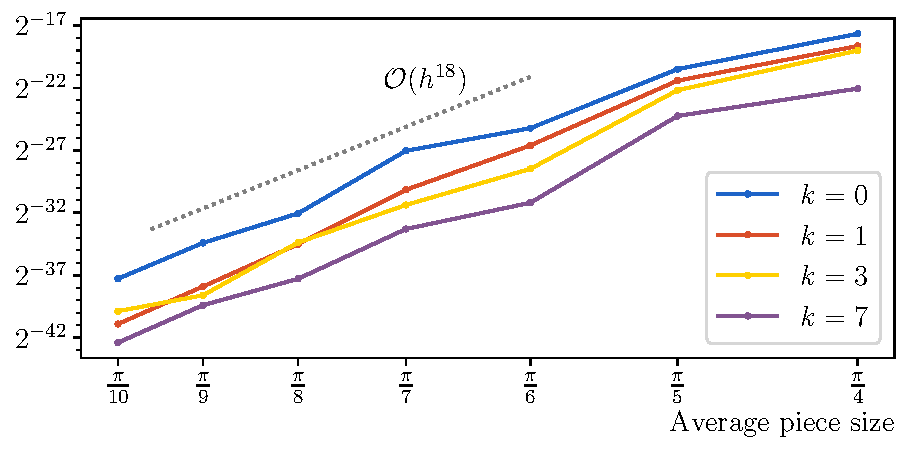
\includegraphics[width=\textwidth]{img/chapter2/matslise_h_error.pdf}
    \end{center}
    \caption{Relative error of the found eigenvalues of problem \eqref{equ:c2_matslise_order_test_problem} by using \matslise{3}.}
    \label{fig:c2_matslise_h_error}
\end{figure}

\begin{figure}
    \begin{center}
        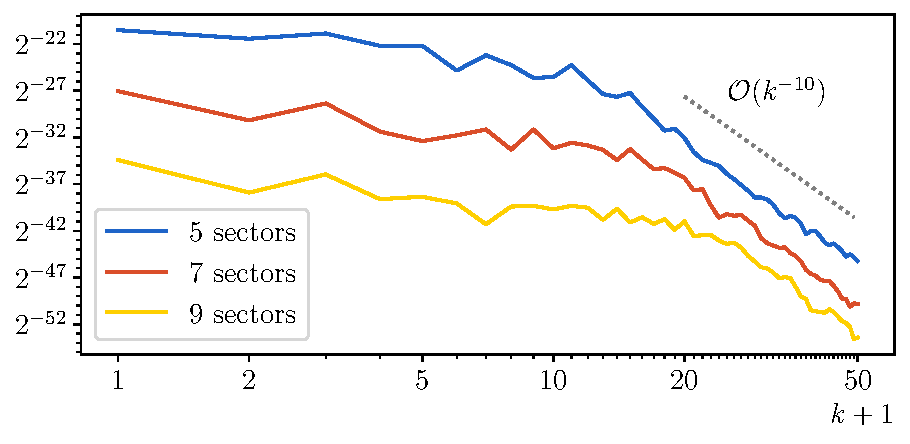
\includegraphics[width=\textwidth]{img/chapter2/matslise_k_error.pdf}
    \end{center}
    \caption{Relative error of the found eigenvalues of problem \eqref{equ:c2_matslise_order_test_problem} by using \matslise{3}. The graphs are in function of the index of the eigenvalue.}
    \label{fig:c2_matslise_k_error}
\end{figure}

To generate figures \ref{fig:c2_matslise_h_error} and \ref{fig:c2_matslise_k_error} we have solved $100$ times the test problem with different tolerances between $2^{-10} \approx 10^{-3}$ and $2^{-30} \approx 10^{-9}$, we have grouped the errors of each of these solves by the number of subintervals \matslise{3} used, and averaged them for each eigenvalue.

In figure \ref{fig:c2_matslise_h_error} we see that the number of subintervals varied between $4$ and $10$. Unsurprisingly, if \matslise{} used more subintervals, the results were more accurate. From the theory, we know that the propagation error from the constant perturbation method $\text{CPM}\{18\}$ is of the order $\OO(h^{18})$. We notice this same order in the error on the eigenvalue.

From the theory we know little about the error estimate with respect to $k$. In theorem \ref{the:c2_pruess_1973_2} we learned that for the Pruess method this order was $\OO(k^{-4})$. With \matslise{} we observe a much more considerable value, visually we suspect this to be $\OO(k^{-9})$ or $\OO(k^{-10})$.

These numerical experiments may serve as a kind of tutorial to get to know \pyslise{}. So we will provide the code each time to solve the problem at hand. Here, to generate the first fifty eigenvalues the following code can be used.
% \begin{noindent}
\begin{minted}{python}
from pyslise import Pyslise
from math import pi, cos

V = lambda x: 100*cos(x)**2

problem = Pyslise(V, 0, pi, tolerance=1e-12)
print(problem.eigenvaluesByIndex(0, 50, (0, 1), (0, 1)))
\end{minted}
% \end{noindent}

The first few lines imports the necessary functions. The next line defines the potential $V(x)$. Then, a \texttt{Pyslise} object is constructed. Here the user needs to provide the potential $V(x)$, and the left ($0$) and right ($\pi$) boundaries of the domain. Optionally a tolerance may be specified. Because we are working in \texttt{double} precision in \lpython{}, anything less than approximately $10^{-16}$ is nonsensical.

Next, we find the eigenvalues. For this we use \texttt{.eigenvaluesByIndex}, a function defined on \texttt{Pyslise} objects. This function expects four arguments: $i_\text{min}$, $i_\text{max}$, $\vb{y_a}$ and $\vb{y_b}$. It will return all eigenvalues $\lambda_i$ for which $i_\text{min} \leq i < i_\text{max}$ of the problem with boundary conditions
$$
    \begin{pmatrix}y(a) \\ y'(a)\end{pmatrix} = s_a \vb{y_a} \quad\text{and}\quad \begin{pmatrix}y(b) \\ y'(b)\end{pmatrix} = s_b \vb{y_b}\text{.}
$$
In this expression are $s_a$ and $s_b$ some scaling factors. Note that providing boundary conditions like this is different from the more mathematical notation
$$
    \alpha_a y(a) + \beta_a y'(a) = 0\text{.}
$$
Our program expects a vector $\vb{y_a} = \begin{pmatrix}\beta_a & - \alpha_a\end{pmatrix}^\transposesign{}$, and analogous for $\vb{y_b}$. We have chosen for these types of arguments to be more in line with how propagation is executed in the constant perturbation method.

\subsection{A potential with jumps}\label{sec:c2_experiment_with_jumps}

In the next numerical experiment we demonstrate another feature of constant perturbation methods. Since the potential function is piecewisely approximated, the potential may be discontinuous as long as the jumps are situated on the boundary between two consecutive subintervals.

Consider the Schrödinger problem with homogeneous Dirichlet boundary conditions on the interval $[-2, 2]$ with potential function
\begin{equation}\label{equ:c2_matslise_jumps_well}
    V(x) = \begin{cases}
        0  & \text{if $|x| \leq 1$} \\
        30 & \text{otherwise.}
    \end{cases}
\end{equation}

\begin{figure}
    \begin{center}
        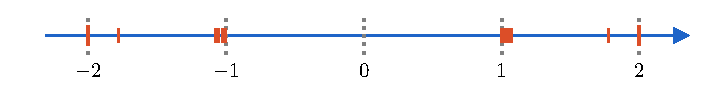
\includegraphics[width=\textwidth]{img/chapter2/matslise_jumps_without.pdf}
    \end{center}
    \caption{Visualization of the subintervals chosen by \matslise{3} for the problem with potential \eqref{equ:c2_matslise_jumps_well}, \emph{without} specifying jumps.}
    \label{fig:c2_matslise_jumps_without}
    \vspace{8mm}
    \begin{center}
        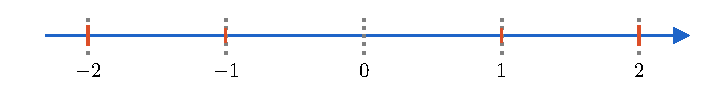
\includegraphics[width=\textwidth]{img/chapter2/matslise_jumps_with.pdf}
    \end{center}
    \caption{Visualization of the subintervals chosen by \matslise{3} for the problem with potential \eqref{equ:c2_matslise_jumps_well}, \emph{with} specifying jumps.}
    \label{fig:c2_matslise_jumps_with}
\end{figure}

If we use a similar program as before this may look like the following.
% \begin{noindent}
\begin{minted}{python}
from pyslise import Pyslise

def V(x):
    return 0 if abs(x) < 1 else 30

problem = Pyslise(V, -2, 2, tolerance=1e-12)
print(problem.eigenvaluesByIndex(0, 5, (0, 1), (0, 1)))
\end{minted}
% \end{noindent}
This program gives the correct results, but it used $15$ subintervals. Those intervals are visualized in figure \ref{fig:c2_matslise_jumps_without}. If we change the line with the construction of the \texttt{Pyslise} object to
% \begin{noindent}
\begin{minted}{python}
problem = Pyslise(V, -2, 2, tolerance=1e-12, jumps=[-1, 1])
\end{minted}
% \end{noindent}
only $3$ subintervals are used. For completeness, we have visualized these 3 subintervals in figure \ref{fig:c2_matslise_jumps_with}. As one may expect, using fewer intervals speeds up the method significantly.

\begin{figure}
    \begin{center}
        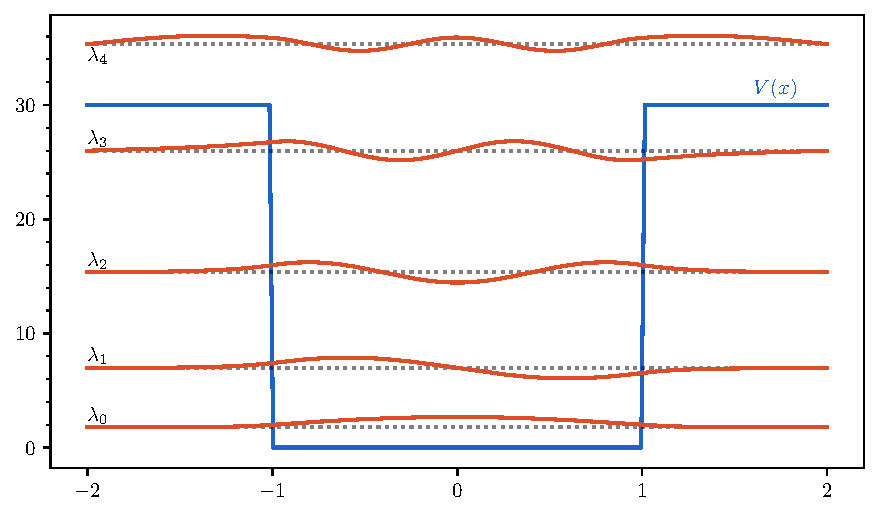
\includegraphics[width=\textwidth]{img/chapter2/matslise_jumps_eigenfunctions.pdf}
    \end{center}
    \caption{These are the first five eigenfunctions of the Schrödinger problem with potential \eqref{equ:c2_matslise_jumps_well}.}
    \label{fig:c2_matslise_jumps_eigenfunctions}
\end{figure}

In any case, the first five eigenfunctions of this Schrödinger problem can be visualized with the following code.
% \begin{noindent}
\begin{minted}{python}
import numpy as np

x = np.linspace(-2, 2, 200)

plt.plot(x, np.vectorize(V)(x))
for i, E, f in problem.eigenpairsByIndex(0, 5, (0, 1), (0, 1)):
    plt.plot(x, E + f(x)[0,:])
\end{minted}
% \end{noindent}
This yields a similar image to figure \ref{fig:c2_matslise_jumps_eigenfunctions}. In this code, \texttt{.eigenpairsByIndex} is a function which expects the same arguments as \texttt{.eigenvaluesByIndex}. But this function returns a list with for each found eigenvalue a tuple with three elements: the index \texttt{i}, the eigenvalue \texttt{E} and the eigenfunction \texttt{f}. This \texttt{f} can be treated as any \lpython{} function, and be evaluated in any value $x$ inside the domain to get the value of the eigenfunction $f(x)$ and its derivative $f'(x)$.

\subsection{Mathieu's equation}\label{sec:c2_numerical_experiments_mathieu}

In the next examples we will compare the numerical accuracy of our new implementation \matslise{3} (and the \lpython{} package \pyslise{}) with the original well-established \matslise{2}.

As a first direct comparison, we will take a look at Mathieu's equation \cite{pryce_sltstpak_1999} on $[0, \pi]$ with homogeneous Dirichlet boundary conditions: \begin{equation}
    \dv[2]{y}{x} + 2q\cos(2x)y(x) = \lambda y(x) \text{.}\label{equ:c2_mathieu_equation}
\end{equation}
In this expression $q$ is a parameter, in these experiments we will consider $q=1$ and $q=10$.

By using \pyslise{}, it is not difficult to find the first $10$ eigenvalues of this equation:

% \begin{noindent}
\begin{minted}{python}
from pyslise import Pyslise
from math import pi, cos

q = 1
def V(x):
    return 2*q*cos(2*x)

mathieu = Pyslise(V, 0, pi, tolerance=1e-8)
print(mathieu.eigenvaluesByIndex(0, 10, (0,1), (0,1)))
\end{minted}
% \ebd{noindent}

The results of this computation can be compared with the results from \matslise{2}. For different values of the parameter $q$ ($q = 1$ and $q = 10$), the true eigenvalues (calculated with \matslise{2} and a tolerance of $10^{-14}$) are used to calculate the error of the eigenvalues obtained from \matslise{2} and \pyslise{}, both with a tolerance of $10^{-8}$. The execution times are reported as well. These were calculated using \matlab{}'s \texttt{timeit} function or Python's \texttt{timeit} function. Both execute the code multiple times to account for fluctuations caused by other system load. These comparisons where run on an Intel i7-8700K.

\begin{table}
    \begin{center}
        \begin{tabular}[]{n{3}{13}n{2}{1}n{2}{1}}
          \toprule
          $q=1$               & {\matslise{2}}    & {\pyslise{}}         \\
          \midrule
                              & \multicolumn{1}{c}{$5.33\text{ms}$} & \multicolumn{1}{c}{$0.21\text{ms}$} \\
          -0.1102488169921  & 6.3e-10   & -2.6e-12  \\
          3.9170247729985   & -8.5e-10  & 4.2e-12   \\
          9.0477392598094   & -1.1e-9   & -4.1e-12  \\
          16.0329700814058  & -6.1e-10  & -1.6e-11  \\
          25.0208408232898  & 3.9e-10   & -2.6e-12  \\
          36.0142899106282  & 5.3e-10   & -4.0e-12  \\
          49.0104182494239  & 1.1e-9    & 1.8e-11   \\
          64.0079371892498  & 1.4e-9    & 1.6e-11   \\
          81.0062503266325  & -4.8e-10  & 4.5e-12   \\
          100.0050506751594 & -8.7e-10  & -9.3e-13  \\
          \bottomrule
        \end{tabular}
      \end{center}
    \vspace{5mm}
      \begin{center}
        \begin{tabular}[]{n{3}{13}n{2}{1}n{2}{1}}
          \toprule
          $q=10$              & {\matslise{2}}    & {\pyslise{}}         \\
          \midrule
                              & \multicolumn{1}{c}{$6.74\text{ms}$} & \multicolumn{1}{c}{$0.30\text{ms}$} \\
          -13.9365524792501 & 5.8e-9    & -5.4e-12  \\
          -2.3821582359569  & 2.2e-8    & 2.9e-12   \\
          7.9860691446817   & 4.7e-10   & 1.4e-11   \\
          17.3813806786230  & -3.4e-8   & 6.4e-12   \\
          26.7664263604801  & -3.1e-8   & -8.2e-12  \\
          37.4198587767242  & -4.7e-8   & -5.1e-12  \\
          50.0541572135572  & -2.9e-8   & 1.1e-12   \\
          64.8004402930215  & 2.7e-8    & 4.1e-12   \\
          81.6283131843831  & 2.7e-8    & -3.1e-11  \\
          100.5067694628784 & 4.0e-8    & -7.1e-12  \\
          \bottomrule
        \end{tabular}
      \end{center}
  \caption{The first 10 eigenvalues for the Mathieu problem~(\ref{equ:c2_mathieu_equation}) for $q=1$ and $q=10$, the execution times and the absolute errors obtained with \matslise{2} and \pyslise{} with a tolerance of $10^{-8}$.}\label{tab:c2_tab1}
\end{table}

From Table~\ref{tab:c2_tab1} there are two things to note. Firstly \pyslise{} is more than 20 times faster than \matslise{2}. This means that our efforts to improve efficiency are definitely worth it.

Secondly the accuracy of \pyslise{} is a lot higher. This can be explained by the fact that \pyslise{}'s error estimates are very conservative. The error estimation is used to choose the mesh to use. Because \pyslise{}'s errors are less sharp, it tends to use more subintervals than \matslise{2}. These extra intervals lead to more accurate results. These more accurate results may seem like a benefit, in reality, it is not. We requested an accuracy for both programs of $10^{-8}$, and \matslise{2} respects this beautifully. In other words \matslise{2} is able to use the lowest number of subintervals possible, while respecting the requested accuracy. \pyslise{} on the other hand, goes above and beyond to ensure the requested accuracy and overshoots it with quite a lot. This means that it uses more subintervals than necessary, and is therefor a little less efficient than it could be.

In practice, and for our use-cases in the following chapters, we have found \matslise{3} and \pyslise{} to be sufficiently fast. Knowing this we decided to keep our error estimate as it is, even though it is more conservative than it needs to be.

\paragraph{Eigenfunctions} As explained in section \ref{sec:c2_cp_in_delta} one of the reasons we developed more complicated formulae and build a new implementation was the evaluation of the eigenfunctions. To evaluate the eigenfunction in \matslise{2}, the partition of the domain has to be recomputed to include the requested evaluation points. If there are only a limited set of points, and these are known beforehand, then \matslise{2}'s methods is sufficient. In many applications however, this is insufficient.

Assume\footnote{Or take a look at section \ref{sec:c3_calculate_vk}, where we need to do exactly this.} we want to compute an orthogonal projection of a function $f(x)$ to the truncated basis of the eigenfunctions $y_i$: $ f(x) = \sum_{i = 0} c_i y_i(x)$.
To compute these numerically we need to approximate the following integrals for all necessary values for $i$:
$$
\int_a^b f(x) y_i(x)\,\dd x\text{.}
$$
In \matslise{2.0}, one would choose a fixed grid beforehand and evaluate all eigenfunctions in exactly these grid points. To approximate the integral, any quadrature rule can be used, as long as it only uses the values in exactly these grid points. If a large basis is used, or $f(x)$ is unpredictable with some steep regions for example, this approach will only be accurate if a prohibitively dense grid is used. Ideally some adaptive quadrature rule should be used. These numerical integration techniques evaluate the integrand in as many values as needed to ensure accuracy. When the integrand becomes `difficult', more evaluations points are dynamically chosen. In the regions where the integrand is `easy', much fewer evaluations are used. But, these methods, of course, need a way to evaluate the integrand dynamically, and do not work with a fixed grid. With this application in mind, our new implementation already has the benefit of being able to do this, with relatively little computational cost. But to see the true power of \matslise{3}, we compare the computation time for the evaluation of eigenfunctions with \matslise{2}. These results are reported in Table~\ref{tab:c2_tab2}.

\begin{table}
  \begin{center}
    \begin{tabular}{rrrr}
      \toprule
      $q = 1$      & $n=100$          & $n=1000$        & $n=10000$        \\
      \midrule
      \matslise{2} & $65.3\text{ms}$  & $647\text{ms}$  & $10180\text{ms}$ \\
      \pyslise{}      & $0.387\text{ms}$ & $3.05\text{ms}$ & $29.3\text{ms}$  \\
      \bottomrule
    \end{tabular}
  \end{center}
  \caption{\label{tab:c2_tab2} Execution times needed to compute the first 10 eigenfunctions of the Mathieu problem~(\ref{equ:c2_mathieu_equation}) in $n$ equidistant points.}
\end{table}

\begin{table}
    \begin{center}
        \begin{tabular}{rn{2}{1}n{2}{1}n{2}{1}n{2}{1}}
          \toprule
                & \multicolumn{1}{c}{$y_{0}$} & \multicolumn{1}{c}{$y_{1}$} & \multicolumn{1}{c}{$y_{2}$} & \multicolumn{1}{c}{$y_{3}$} \\
          \midrule  
          \matslise{2}    & 1.0e-10 & 6.2e-9 & 1.7e-10 & 1.4e-9   \\
          \pyslise{}      & 4.7e-9 & 5.9e-9 & 2.8e-9 & 1.9e-9   \\
          \midrule
          \midrule
            &\multicolumn{1}{c}{$y_{4}$}    & \multicolumn{1}{c}{$y_{5}$} & \multicolumn{1}{c}{$y_{6}$} & \multicolumn{1}{c}{$y_{7}$} \\
          \midrule
          \matslise{2}    & 4.0e-11 & 5.7e-10 & 8.2e-11 & 8.6e-10  \\
          \pyslise{}      & 3.9e-9 & 2.6e-9 & 1.4e-9 & 1.3e-9   \\
          \bottomrule
        \end{tabular}
      \end{center}
  \caption{\label{tab:c2_tab3} Maximum absolute error in $n=100$ equidistant points of the eigenfunction $y_n$ corresponding to $\lambda_n$ for the Mathieu problem (\ref{equ:c2_mathieu_equation}) with $q=1$.}
\end{table}

In this scenario the difference in efficiency becomes apparent. \pyslise{} is two orders of magnitude faster than \matslise{2}. On top of that, this extreme speedup is achieved without dropping below the requested accuracy. In table~\ref{tab:c2_tab3} the maximum error of the eigenfunction for each eigenvalue is tabulated. One notices that \matslise{2} is more accurate, but remember that the requested accuracy in this experiment was for both programs $10^{-8}$. As long as the results are more accurate than $10^{-8}$, they are successful.

It is remarkable that for the eigenvalues $\pyslise{}$ was more accurate than required. For the eigenfunctions, the situation is reversed. This reversion can be explained by the fact that \pyslise{} is able to reuse the same grid (which was accurate to the required tolerance), but \matslise{2} computes a new partition with the grid points used for the computation of the eigenvalue together with all requested evaluation points of the eigenfunction. This grid is much denser, and thus unnecessarily more accurate.

\subsection{Coffey-Evans problem}\label{sec:c2_numerical_experiments_coffey_evans}

Another, more challenging problem is the Coffey-Evans equation \cite{pryce_error_1986}.
\begin{equation}
  -y''(x) + (\beta^2\sin^2(2x)-2\beta\cos(2x))y(x) = \lambda y(x)\text{,}\label{equ:c2_coffey_evans}
\end{equation}
with $x \in [-\frac{\pi}{2}, \frac{\pi}{2}]$ and homogeneous Dirichlet boundary condition.

The Coffey-Evans equation has two interesting features: firstly it is a symmetric problem, secondly it has triplets of close eigenvalues and the closeness increases dramatically as the parameter $\beta$ increases. Accurately discriminating these close but different eigenvalues is a challenge.

To exploit this symmetry \texttt{PysliseHalf} can be used. Besides this, the few lines of Python needed to find the first eigenvalues are very similar to the other examples.

% \begin{noindent}
\begin{minted}{python}
from pyslise import PysliseHalf
from math import pi, sin, cos

beta = 15
def V(x):
    return beta**2 * sin(2*x)**2 - 2*beta * cos(2*x)

coffey_evans = PysliseHalf(V, pi/2, tolerance=1e-8)
print(coffey_evans.eigenvaluesByIndex(0, 10, (0,1)))
\end{minted}
% \end{noindent}

In the last line we notice that supplying only one boundary condition is sufficient; symmetric boundary conditions are expected when using a half-range reduction. In table \ref{tab:c2_tab4} we present, for $\beta=5$, $\beta=15$ and $\beta=25$ the results of our experiment. Here the reference values of the first nine eigenvalues are computed with \matslise{2} with a tolerance of $10^{-14}$. In the next column the errors obtained with \matslise{2} and a tolerance of $10^{-8}$ are given. And in the last column, the errors of \pyslise{} with the same tolerance of $10^{-8}$ are presented.

Besides the numerical results, also the computational running time is reported in table \ref{tab:c2_tab4}. Similarly to the results from the Mathieu problem, \pyslise{} was significantly faster and more accurate. But in contrast to the previous example, now one could argue that \matslise{2} no longer respects the requested accuracy of $10^{-8}$ for $\beta = 25$. However, the relative error is sufficiently small.

\begin{table}
    \begin{center}
        \begin{tabular}[]{n{1}{0}n{3}{13}n{2}{1}n{2}{1}}
            \toprule
              & {$\beta=5$}       & {\matslise{2}}                       & {\pyslise{}}                        \\
            \midrule
              &                   & \multicolumn{1}{c}{$8.94\text{ms}$}  & \multicolumn{1}{c}{$0.33\text{ms}$} \\
            0 & 0.0005463030588   & 4.5e-1                               & 2.4e-10                             \\
            1 & 17.4201300751401  & 3.1e-9                               & 1.4e-11                             \\
            2 & 26.8313294875207  & 8.2e-9                               & 5.2e-12                             \\
            3 & 30.6514597044625  & 1.1e-9                               & -3.2e-12                            \\
            4 & 37.9709848127178  & -1.6e-8                              & 9.2e-12                             \\
            5 & 49.4100375966783  & -6.0e-9                              & -1.8e-11                            \\
            6 & 62.2115039443358  & -6.7e-9                              & -3.7e-12                            \\
            7 & 76.9997687851650  & -3.1e-8                              & -4.1e-11                            \\
            8 & 93.8923408372478  & -1.5e-8                              & -4.5e-11                            \\
            \bottomrule
            \toprule
              & {$\beta=15$}      & {\matslise{2}}                       & {\pyslise{}}                        \\
            \midrule
              &                   & \multicolumn{1}{c}{$9.71\text{ms}$}  & \multicolumn{1}{c}{$0.54\text{ms}$} \\
            0 & 0.0000000000035   & -1.7e-7                              & -1.1e-11                            \\
            1 & 57.8833068486108  & 3.2e-7                               & 4.8e-11                             \\
            2 & 111.2023333512293 & 1.9e-7                               & 1.1e-10                             \\
            3 & 111.2270694418592 & 3.1e-7                               & 4.9e-11                             \\
            4 & 111.2518808183127 & 1.9e-7                               & 1.1e-10                             \\
            5 & 159.1826724323144 & 5.3e-9                               & 1.7e-10                             \\
            6 & 197.3328583631476 & 6.3e-8                               & -7.5e-11                            \\
            7 & 199.8690055338356 & 2.6e-9                               & 6.3e-13                             \\
            8 & 203.2295295020015 & 2.7e-8                               & -2.1e-10                            \\
            \bottomrule
            \toprule
              & {$\beta=25$}      & {\matslise{2}}                       & {\pyslise{}}                        \\
            \midrule
              &                   & \multicolumn{1}{c}{$24.36\text{ms}$} & \multicolumn{1}{c}{$0.61\text{ms}$} \\
            0 & -0.0000000000000  & -4.4e-7                              & -2.4e-11                            \\
            1 & 97.9345616863637  & 7.9e-7                               & -3.2e-11                            \\
            2 & 191.5876270396656 & 8.3e-7                               & 4.8e-11                             \\
            3 & 191.5876332913999 & 1.2e-6                               & -1.3e-11                            \\
            4 & 191.5876395431371 & 7.2e-7                               & 4.6e-11                             \\
            5 & 280.6142452706786 & 1.7e-7                               & 1.7e-10                             \\
            6 & 364.5514239171786 & 6.2e-8                               & -4.4e-12                            \\
            7 & 364.5556442011433 & -8.5e-8                              & 2.2e-10                             \\
            8 & 364.5598657470625 & 6.1e-8                               & 2.4e-10                             \\
            \bottomrule
        \end{tabular}
    \end{center}
    \caption{Eigenvalues for the Coffey-Evans problem~(\ref{equ:c2_coffey_evans}), with absolute errors obtained by \matslise{2} and \pyslise{} with a tolerance of $10^{-8}$.}\label{tab:c2_tab4}
\end{table}

\begin{table}
    \begin{center}
        \begin{tabular}{rn{2}{1}n{2}{1}n{2}{1}n{2}{1}}
            \toprule
            {$\beta=5$}    & \multicolumn{1}{c}{$y_{0}$} & \multicolumn{1}{c}{$y_{1}$} & \multicolumn{1}{c}{$y_{2}$} & \multicolumn{1}{c}{$y_{3}$} \\
            \midrule
            {\matslise{2}} & 2.0e-11                     & 3.2e-10                     & 1.5e-9                      & 2.1e-10                     \\
            {\pyslise{}}   & 4.2e-9                      & 8.5e-10                     & 1.4e-9                      & 1.4e-9                      \\
            \midrule
            \midrule
            {$\beta=5$}    & \multicolumn{1}{c}{$y_{4}$} & \multicolumn{1}{c}{$y_{5}$} & \multicolumn{1}{c}{$y_{6}$} & \multicolumn{1}{c}{$y_{7}$} \\
            \midrule
            {\matslise{2}} & 1.5e-9                      & 5.4e-10                     & 5.0e-10                     & 2.2e-9                      \\
            {\pyslise{}}   & 1.9e-9                      & 1.4e-9                      & 1.8e-9                      & 1.8e-9                      \\
            \bottomrule
        \end{tabular}
    \end{center}
    \vspace{8mm}
    \begin{center}
        \begin{tabular}{rn{2}{1}n{2}{1}n{2}{1}n{2}{1}}
            \toprule
            {$\beta=15$}   & \multicolumn{1}{c}{$y_{0}$} & \multicolumn{1}{c}{$y_{1}$} & \multicolumn{1}{c}{$y_{2}$} & \multicolumn{1}{c}{$y_{3}$} \\
            \midrule
            {\matslise{2}} & 2.8e-9                      & 1.2e-8                      & 4.0e-6                      & 1.7e-5                      \\
            {\pyslise{}}   & 2.0e-10                     & 7.3e-10                     & 4.6e-9                      & 5.7e-9                      \\
            \midrule
            \midrule
            {$\beta=15$}   & \multicolumn{1}{c}{$y_{4}$} & \multicolumn{1}{c}{$y_{5}$} & \multicolumn{1}{c}{$y_{6}$} & \multicolumn{1}{c}{$y_{7}$} \\
            \midrule
            {\matslise{2}} & 4.0e-6                      & 1.8e-10                     & 1.2e-8                      & 1.1e-9                      \\
            {\pyslise{}}   & 3.5e-9                      & 2.3e-9                      & 2.2e-9                      & 3.3e-9                      \\
            \bottomrule
        \end{tabular}
    \end{center}
    \vspace{8mm}
    \begin{center}
        \begin{tabular}{rn{2}{1}n{2}{1}n{2}{1}n{2}{1}}
            \toprule
            {$\beta=25$}   & \multicolumn{1}{c}{$y_{0}$} & \multicolumn{1}{c}{$y_{1}$} & \multicolumn{1}{c}{$y_{2}$} & \multicolumn{1}{c}{$y_{3}$} \\
            \midrule
            {\matslise{2}} & 4.6e-9                      & 1.9e-8                      & 8.2e-2                      & 3.1e-1                      \\
            {\pyslise{}}   & 2.0e-10                     & 6.9e-10                     & 7.0e-6                      & 6.5e-6                      \\
            \midrule
            \midrule
            {$\beta=25$}   & \multicolumn{1}{c}{$y_{4}$} & \multicolumn{1}{c}{$y_{5}$} & \multicolumn{1}{c}{$y_{6}$} & \multicolumn{1}{c}{$y_{7}$} \\
            \midrule
            {\matslise{2}} & 6.5e-2                      & 3.7e-9                      & 7.8e-6                      & 2.9e-5                      \\
            {\pyslise{}}   & 7.0e-6                      & 2.2e-9                      & 2.8e-8                      & 2.7e-9                      \\
            \bottomrule
        \end{tabular}
    \end{center}
    \caption{\label{tab:c2_ce_eigenfunctions} Maximum error in $100$ equidistant points of the eigenfunction corresponding to each of first eight eigenvalues for the Coffey-Evans problem (\ref{equ:c2_coffey_evans}) with $\beta=5$, $\beta=15$ and $\beta=25$.}
\end{table}

\begin{figure}
    \begin{center}
        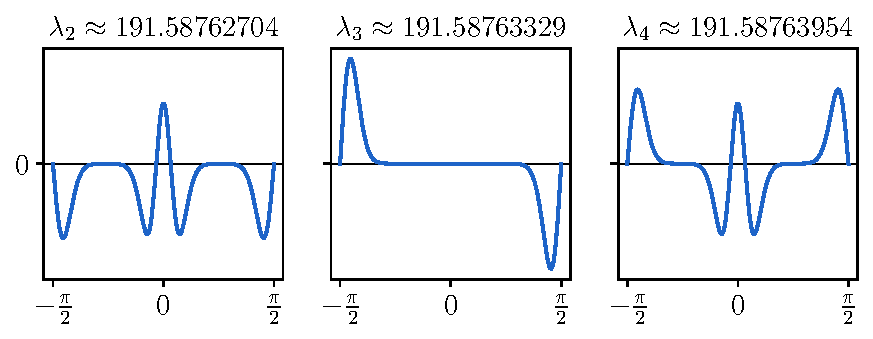
\includegraphics[width=1\textwidth]{img/chapter2/pyslise_test/coffey_evans_eigenfunctions.pdf}
    \end{center}
    \caption{A plot of the eigenfunctions $y_2$, $y_3$ and $y_4$ of the Coffey-Evans problem~(\ref{equ:c2_coffey_evans}) with $\beta=25$.}\label{fig:coffey_evans_eigenfunctions}
\end{figure}

As seen previously, eigenfunctions can be visualized. If we want to recreate graphs similar to figure \ref{fig:coffey_evans_eigenfunctions}, the following code can be used.
% \begin{noindent}
\begin{minted}{python}
import matplotlib.pyplot as plt
import numpy as np

x = np.linspace(-pi/2, pi/2, 200)

for i, E, f in coffey_evans.eigenpairsByIndex(2, 5, (0, 1)):
    plt.plot(x, f(x)[0,:])
    plt.show()
\end{minted}
% \end{noindent}
Notice here that by providing the arguments \texttt{2} and \texttt{5} to \texttt{.eigenpairsByIndex}, we only request the eigenvalues and eigenfunctions with index $2$, $3$ and $4$. Visually these graphs look convincing. But, as a more rigorous verification we have provided table \ref{tab:c2_ce_eigenfunctions}. Here the maximum absolute errors in the eigenfunctions are tabulated. Again, we have used \matslise{2} with a tolerance of $10^{-14}$ to obtain reference results to compare with.

\todo{Maybe something about orthogonality}

From the theory we expect that the time needed to evaluate the eigenfunction does not depend on the difficulties to find eigenvalues for that particular problem. Once an eigenvalue is found, the corresponding eigenfunction should be easily calculated. The computation time to evaluate an eigenfunction for an equidistant grid of $n$ points is reported in table \ref{tab:c2_tab6}. The remarkable speed-up we were able to achieve with our new implementation can be observed.

\begin{table}
    \begin{center}
        \begin{tabular}{rrrr}
            \toprule
            $\beta = 15$ & $n=100$          & $n=1000$        & $n=10000$       \\
            \midrule
            \matslise{2} & $59.9\text{ms}$  & $525\text{ms}$  & $7508\text{ms}$ \\
            \pyslise{}   & $0.344\text{ms}$ & $2.58\text{ms}$ & $24.5\text{ms}$ \\
            \bottomrule
        \end{tabular}
    \end{center}
    \caption{\label{tab:c2_tab6} Maximum error in $n$ equidistant points of the eigenfunction $y_n$ for the Coffey-Evans problem (\ref{equ:c2_coffey_evans}) with $\beta=15$.}
\end{table}

\subsection{Truncated hydrogen potential}\label{sec:c2_numerical_experiments_hydrogen}

As a next example we will take a look at the truncated hydrogen potential \cite{pryce_sltstpak_1999}:
\begin{equation}
    V(x) = -\frac{1}{x} + \frac{2}{x^2}\text{,} \label{equ:c2_truncated_hydrogen}
\end{equation}
on the domain $[0, 1000]$ with homogeneous Dirichlet boundary conditions. The lower eigenvalues are a good approximation for the eigenvalues of the non-truncated problem (on the domain $x \in \left[0, \infty\right[$). By now, the code to solve this problem may seem very familiar.

% \begin{noindent}
\begin{minted}{python}
from pyslise import Pyslise

def V(x):
    return -1/x + 2/x**2

hydrogen = Pyslise(V, 0, 1000, tolerance=1e-8)
print(hydrogen.eigenvaluesByIndex(0, 10, (0, 1), (0, 1)))
\end{minted}
% \end{noindent}

The potential is unbounded for the left endpoint of the integration interval, thus this is a singular problem. \matslise{2} is well-suited for singular problems. It contains many checks to identify and routines to work around singularities of the problem. For efficiency reasons, \pyslise{} does not have these extra features.

Despite these missing features, \pyslise{} can still solve the problem. And, it is even faster and more accurate. We do note that speedup is less significant than for non-singular problems. In table \ref{tab:c2_tab7} we see that \pyslise{} is at least as accurate as Matslise and approximately 4 times faster (in contrast to 20 times for the Mathieu en Coffey-Evans problems).

\begin{table}
    \begin{center}
        \begin{tabular}[]{n{2}{13}n{2}{1}n{2}{1}}
            \toprule
                             & \matslise{2}       & \pyslise{}        \\
            \midrule
                             & {$30.96\text{ms}$} & {$7.09\text{ms}$} \\
            -0.0625000000000 & 2.1e-12            & 8.9e-15           \\
            -0.0277777777778 & 4.9e-12            & -2.2e-15          \\
            -0.0156250000000 & 3.4e-12            & -9.0e-16          \\
            -0.0100000000000 & 9.4e-13            & -2.7e-15          \\
            -0.0069444444444 & -1.1e-12           & 1.2e-13           \\
            -0.0051020408163 & -2.3e-12           & -6.3e-13          \\
            -0.0039062500000 & -2.9e-12           & -2.3e-13          \\
            -0.0030864197531 & -3.0e-12           & 1.1e-13           \\
            -0.0025000000000 & -2.7e-12           & -9.6e-14          \\
            -0.0020661157025 & -1.9e-12           & 1.6e-14           \\
            \bottomrule
        \end{tabular}
        \caption{The first ten eigenvalues for the truncated hydrogen problem~(\ref{equ:c2_truncated_hydrogen}), the execution times and the errors obtained with \matslise{2} and \pyslise{} for a tolerance of $10^{-8}$.}\label{tab:c2_tab7}
    \end{center}
\end{table}

For the evaluation of the eigenfunctions, this singularity does not matter. The eigenfunctions are evaluated with a maximal error of less than $10^{-9}$, with timings similar to the previous test problems.

\subsection{Periodic problem with an asymmetric potential}\label{sec:c2_experiments_andrew_periodic}

As described in section \ref{sec:c2_periodic}, \matslise{3} is able to solve Schrödinger problems with periodic boundary conditions. To demonstrate this we will solve a problem also found in \cite{andrew_correction_1989}. Consider the Schrödinger equation
$$
    -y''(x) + x^2(\pi-x) y(x) = \lambda y(x)
$$
on the domain $[0, \pi]$ with periodic boundary conditions: $y(0) = y(\pi)$ and $y'(0) = y'(\pi)$.

To solve this with \pyslise{} we need to import a different solver, but most of the code is similar.
% \begin{noindent}
\begin{minted}{python}
from pyslise import PyslisePeriodic
from math import pi

def V(x):
    return x*x*(pi-x)

problem = PyslisePeriodic(V, 0, pi, tolerance=1e-8)

print(problem.eigenvaluesByIndex(0, 20))
\end{minted}
% \end{noindent}

In this code there are two notable differences to previous examples. First, \texttt{PyslisePeriodic} is used as solver. And second, no boundary conditions are provided to the \texttt{.eigenvaluesByIndex} function. These are unnecessary because periodic boundary conditions are implied by \texttt{PyslisePeriodic}.

Another difference can be found in the output:
% \begin{noindent}
\begin{minted}{python}
[
    (0, 2.0294161514952878, 1), (1, 6.500490696092834, 1),
    ...,
    (18, 326.5881759903209, 1), (19, 402.5834632545595, 1)
]
\end{minted}
% \end{noindent}

The function \texttt{.eigenvaluesByIndex} returns a list of all found eigenvalues. Now for each eigenvalue the tuple has three elements: the index, the eigenvalue and the multiplicity. From the theory we know that for periodic problems eigenvalues must no longer be unique. An eigenvalue can have a double multiplicity, if \pyslise{} detects this, a multiplicity of $2$ is returned. For example, if we request much higher eigenvalues with the line
% \begin{noindent}
\begin{minted}{python}
print(problem.eigenvaluesByIndex(1000, 1005))
\end{minted}
% \end{noindent}
then the following output is generated.
% \begin{noindent}
\begin{minted}{python}
[
    (999, 1000002.5873939216, 2), (1001, 1004006.5873655227, 2),
    (1003, 1008018.5849614257, 2), (1005, 1012038.5812170412, 2)
]
\end{minted}
% \end{noindent}
These higher eigenvalues are degenerate, so \pyslise{} returns multiplicity $2$. This can also be seen in the index of the returned eigenvalues.

\begin{table}
    \begin{center}
        \begin{tabular}{n{2}{0}n{3}{4}n{3}{5}n{3}{12}}
\toprule
& {Andrew\cite{andrew_correction_1989}} & {Vanden Berghe\cite{vandenberghe_modified_1995}} & {\pyslise{} ($10^{-12}$)} \\
\midrule
0 &  &  & 2.029416151495 \\
1 & 6.5005 & 6.50049 & 6.500490696093 \\
2 & 7.0151 & 7.01506 & 7.015056863171 \\
3 & 18.5848 & 18.58477 & 18.584772142361 \\
4 & 18.6655 & 18.66548 & 18.665481445221 \\
5 & 38.5816 & 38.58162 & 38.581627865277 \\
6 & 38.6215 & 38.62154 & 38.621542547363 \\
7 & 66.5821 & 66.58204 & 66.582047792290 \\
8 & 66.6054 & 66.60537 & 66.605365007694 \\
9 & 102.5825 & 102.58252 & 102.582525988841 \\
10 & 102.5977 & 102.59772 & 102.597720549763 \\
11 & 146.5829 & 146.58286 & 146.582865091809 \\
12 & 146.5935 & 146.59352 & 146.593522877933 \\
13 & 198.5831 & 198.58310 & 198.583098056935 \\
14 & 198.5910 & 198.59998 & 198.590975696561 \\
15 & 258.5833 & 258.58326 & 258.583260746092 \\
16 & 258.5893 & 258.58931 & 258.589315759431 \\
17 & 326.5834 & 326.58338 & 326.583377751489 \\
18 & 326.5882 & 326.58817 & 326.588175990321 \\
19 & 402.5835 & 402.58347 & 402.583463254559 \\
\bottomrule
\end{tabular}

    \end{center}
    \caption{The first 20 eigenvalues for the periodic problem from section \ref{sec:c2_experiments_andrew_periodic}.}\label{tab:c2_andrew_periodic}
\end{table}

\begin{figure}
    \begin{center}
        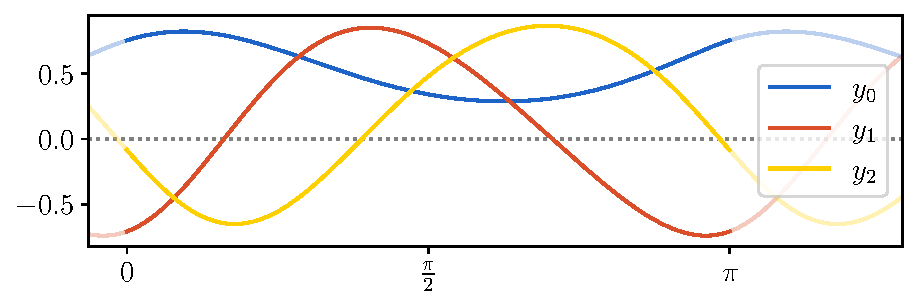
\includegraphics[width=1\textwidth]{img/chapter2/matslise_periodic_eigenfunctions.pdf}
    \end{center}
    \caption{A plot of the first three eigenfunctions $y_0$, $y_1$ and $y_2$ with eigenvalues $\lambda_0\approx\numprint{2.029}$, $\lambda_1\approx\numprint{6.500}$ and $\lambda_0\approx\numprint{7.015}$ of  the periodic problem from section \ref{sec:c2_experiments_andrew_periodic}.}\label{fig:c2_periodic_eigenfunctions}
\end{figure}

In \cite{andrew_correction_1989} the first twenty eigenvalues are computed to four digits behind the decimal point. In \cite{vandenberghe_modified_1995} an extra fifth digit is computed. \matslise{3} can be much more accurate. In table \ref{tab:c2_andrew_periodic} we have tabulated the results from \cite{andrew_correction_1989}, from \cite{vandenberghe_modified_1995} and the results obtained with \pyslise{} and a tolerance of $10^{-12}$. Our computed values agree with the literature up to all five digits, except for the last eigenvalue where we have found a different rounding.

As an illustration we present the graph of the first three eigenfunctions in figure \ref{fig:c2_periodic_eigenfunctions}.


\subsection{Sturm-Liouville problems}\label{sec:c2_experiment_sturm_liouville}

As a last example we present the following Sturm-Liouville problem from \cite{siedlecki_sturmliouville_2016}:
$$
    -\left((1+x)^2 y'(x)\right)' + \left(x^2 - 2\right) y(x) = \lambda e^x y(x)
$$
on the domain $[0, 1]$ with a homogeneous Dirichlet boundary condition on the left and a homogeneous Neumann boundary condition on the right: $y(0) = 0$ and $y'(1) = 0$.

Solving this in \pyslise{} can be achieved with the following program.
% \begin{noindent}
\begin{minted}{python}
from pyslise import SturmLiouville
from math import exp

def p(x):
    return (1 + x)**2

def q(x):
    return x * x - 2

def w(x):
    return exp(x)
    
sturm_liouville = SturmLiouville(p, q, w, 0, 1, tolerance=1e-8)
print(sturm_liouville.eigenvaluesByIndex(0, 10, (0, 1), (1, 0)))
\end{minted}
% \end{noindent}

Here we are using the \texttt{SturmLiouville} solver. We now have to specify the three defining functions $p(x)$, $q(y)$ and $w(x)$. Notice that in the last line we have specified $y(0) = 0$ and $y'(0) = 1$ to mark the left boundary condition, and $y(1) = 1$ and $y'(1) = 0$ to mark the right boundary conditions. Remember that solutions will only satisfy these boundary conditions after some scaling factor.

Under the hood, the \texttt{SturmLiouville} solver will compute Liouville's transformation as in section \ref{sec:c2_liouville_transformation}. This yields a Schrödinger problem for which \matslise{3} will use the constant perturbation method, just as for the \texttt{Pyslise} solver.

\begin{table}
    \begin{center}
        \begin{tabular}{n{3}{8}n{3}{12}n{2}{1}}
            \toprule
            {Siedlecki \cite{siedlecki_sturmliouville_2016}} & {\matslise{2}}   & {\pyslise{} error} \\
            \midrule
            1.17049262                                       & 1.170492759902   & 2.2e-12            \\
            26.8633617                                       & 26.863367646410  & 8.3e-12            \\
            78.5490026                                       & 78.549045264140  & 2.4e-12            \\
            156.079996                                       & 156.080156224823 & 7.2e-12            \\
            259.455041                                       & 259.455476210930 & 4.7e-12            \\
            388.673823                                       & 388.674790600773 & 5.7e-12            \\
            543.736155                                       & 543.738037129327 & 5.2e-12            \\
            724.641861                                       & 724.645192282213 & 4.5e-13            \\
            \bottomrule
        \end{tabular}
    \end{center}
    \caption{Comparing numerical results for the problem from section \ref{sec:c2_experiment_sturm_liouville}. In the right most column the absolute error of our implementation with a specified tolerance of $10^{-8}$ are reported.}\label{tab:c2_pyslise_sturm_liouville_errors}
\end{table}

In table \ref{tab:c2_pyslise_sturm_liouville_errors} we have compared the accurate values from \matslise{2} to the reported values in \cite{siedlecki_sturmliouville_2016} and our new implementation. Note that for our implementation the absolute errors are reported, which means that the relative error is close to machine precision.


\section{Matslise 3.0 -- A new implementation}\label{sec:c2_the_implementation}

Later on in chapters \ref{cha:c3} and \ref{cha:c4} we develop methods to solve time-independent two-dimensional Schrödinger problems. These methods will depend upon our ability to solve the one-dimensional problem accurately and efficiently. Not only eigenvalues will be required, but evaluating eigenfunctions will be essential.

This need for speed drove us away from \matslise{} or \matslise{2}. These are efficient and accurate packages which mainly focus on the computation of the eigenvalues with automatic regularity detection. In our case, we need a package that allows the fast and accurate solution of the eigenvalues as well as of the eigenfunctions of regular one-dimensional Schrödinger-problems. We investigate possible bottlenecks of performance of the \matslise{2} package and its routines.

Let us start with the computation of the eigenvalues. The original \matslise{} package as well as its successor \matslise{2} are highly optimized packages, in the sense that they are designed to compute the eigenvalues of various types of regular and irregular Schrödinger and Sturm-Liouville problems as efficiently as possible. For this, only one coarse mesh, typically consisting of only a few mesh points, is determined. The mesh is then used for all eigenvalue computations. This means that all evaluations of the coefficient functions $C_i^(q)$ from theorem \ref{the:c2_perturbation_terms} are performed during the construction of the mesh and are saved for later reuse. This makes the actual computation of the eigenvalues, at least in an interpreted language such \matlab{}, as fast as possible. For the actual computation of the eigenvalues, the main bottleneck of performance of \matslise{2} is \matlab{}. This environment creates an interpreted language which is inherently slower than a compiled one like \fortran{} or \texttt{C}. However, using \matlab{} has the great benefit of being user-friendly. Even less seasoned programmers are able to easily implement their Sturm-Liouville problem. In \matslise{2}, a graphical user interface is provided to aid in specifying the user's problem, without any programming knowledge needed.

Since we wanted to reimplement \matslise{} into a faster compiled language, we had to consider what we would gain but also what we would lose. Speed and efficiency only goes so far if it is implemented in a prohibitively difficult package to use. As stated, one of the great strengths of \matslise{2} is its ease of use. We were hesitant to use compiled languages for this reason.

In the current day and age one of the more popular languages, with a larger community than \fortran{}'s or \matlab{}'s is \lpython{}. Like \matlab{}, this language is interpreted and is thus equally slow \cite{chaves_octave_2006,unpingco_comparative_2008}. However, in \lpython{} it is not hard to add native packages. These packages are not written in \lpython{} but in some other, more low-level, language. This other language is compiled to native machine code, and nicely packaged to be called from within \lpython{}.

These native packages are the answer to the efficiency versus user-friendliness problem we were faced with. The high performing part can be efficiently implemented in a compiled language, but the code that the user will use can be written in the more approachable \lpython{} The last question before we could build our new implementation of Matslise was: ``Which compiled language?''. This language has to be able to support the building of \lpython{} packages, it has to have support for linear algebra, preferably with optimized BLAS libraries, and it has to support code architecture for numerical libraries. All of these requests makes \cpp{} a prime candidate. In combination with \pybind{} \cite{jakob_pybind11_2017} for the \lpython{} compatibility and \Eigen{} v3 \cite{guennebaud_eigen_2010} as linear algebra library we have the perfect tools to satisfy all our needs.

\paragraph{Try it out!} The new implementation, which we called Matslise 3.0, can be accessed and executed in three different ways.

\begin{itemize}
    \item As a \cpp{} program: the source code of the package is hosted at \url{https://github.com/twist-numerical/matslise}. There, instructions to compile it can be found.
    \item As a \lpython{}-package: in order to avoid that users need to compile the packages themselves, we also provide a 64-bit prebuilt python package \pyslise{}, for \texttt{Linux}, \texttt{Windows} and \texttt{macOS}. Installing \pyslise{} is as easy as simply running:
          % \begin{noindent}
\begin{minted}{python}
pip install pyslise
\end{minted}
% \end{noindent}
    \item Online: lastly we also have created the possibility to run this code inside the web browser: \url{https://matslise.ugent.be/ti1d}. See section \ref{sec:c2_online_gui}.
\end{itemize}

\subsection{Implementation challenges}

Building a new implementation from an existing package allows for incorporating some learned lessons from the previous implementations, and simplifying some functionality.  In practice this is harder than it sounds. For example, when simplifying some functionality one has to carefully consider why the original code did not include this simplification. Forgot the original program to consider it? Was it a remnant of a previous version, or removed code? Or something else entirely? In the hard way, I have learned that, in numerical algorithms especially, the original programmer probably had very good reasons not to include something. More times than I would like to admit, I simplified some code for \matslise{2} to include in the new implementation, only to discover that my `simplification' did not cover all edge-cases or all possible scenarios. In the best cases I made these discoveries quickly upon testing that code. Other times these discoveries only occurred a few months or even years later when getting stuck on a particular difficult bug.

In this section we want to highlight some challenges we encountered while building the new implementation. Some of these are a consequence of the choice for language we have made, some are some inherent challenges of the constant perturbation method and others are self-inflicted by the ambitious goals we set out for ourselves.

\todo{About the code-architecture, overview of parts}

\todo{UML diagram}

\subsubsection{Computation of the perturbation term formulae}

In theorem \ref{the:c2_perturbation_terms} a nice procedure is outlined to determine each of the propagators $u(\delta)$ and $v(\delta)$. In short both propagators are written in the following form:
$$
    u(\delta) = \sum_{q = -1}^{Q} c_q(\delta) \eta_{q}(\delta)
$$
with $c_i$ a polynomial in $\delta$,
\begin{equation}\label{equ:c2_symbolic_propagators}
    c_q(\delta)  = \sum_{i=0}^{N} d_{q, i} \delta^i\text{,}
\end{equation}
and $d_{q, i}$ is a polynomial in $h$ with coefficients in $V_1, \dots, V_{N}$.

Once a mesh is constructed and $V_1, \dots, V_{N}$ are determined, the values for $d_{q, i}$ are fixed on each subinterval. This means that these values can be computed once and be reused for each guess for $\lambda$. In practice, the formulae for the values of $d_{i, j}$ are quite complicated. For small values of $N$ and $Q$ it would be feasible to implement these values by hand, for the large $N$ and $Q$ we are using here, this is intractable.

We could compute these formulae each time we construct a mesh by implementing some symbolic computation in \cpp{}. This could work, but it is less than ideal. Not only would this include a large computational burden, it would also be quite labor-intensive to implement the symbolic tools needed to pull this off. A better strategy is to use a symbolic toolbox like \maple{}, \mathematica{}, or \sage{} and let it generate the necessary \cpp{}-code only once before compiling the program. Computing the formulae once and generating code for them  also has the added benefit that the \cpp{} compiler can optimize them and generate the best possible machine-code.

In the appendices of \cite{ledoux_study_2007} some \maple{} programs are present which are able to determine the necessary values if $h = \delta$. For our case, because we want to have these formulae for general $\delta$, a new program needs to be written. In the next chapter, the method we develop also uses constant perturbation formulae for coupled systems of Schrödinger equations, therefor it would also be valuable if this new program is also able to compute these. And lastly, it would be a nice to have if these formulae could be generated in a matter of minutes instead of weeks, for example.

We have implemented this in \sage{} \cite{sagemath}. Here it is possible to precisely specify what type each variable is. Mathematically, all expressions are polynomials in $h$, $\delta$ and $V_0, \dots, V_N$, as such, all computations will be executed in the following polynomial ring:
$$
    \QQ[V_0, \dots, V_n][h][\delta]\text{.}
$$
This means that all expressions in \sage{} will have the following structure with coefficients $r \in \QQ$:
$$
    \sum_i \left(\sum_j \left( \sum_{k_0,\dots, k_N} r_{i,j,k_0,\dots,k_N} V_0^{k_0} \cdots V_N^{k_N}  \right)h^j \right) \delta^i\text{.}
$$
This structure allows \sage{} to optimize each expression, in contrast to working with general symbolic expressions, which would also allow other operations such as division or $\sin$ for example.

As an example, the \sage{} program starts with defining the variables $V_0, \dots, V_N$, $h$ and $\delta$.
%\begin{noindent}
\begin{minted}{python}
pr_V = QQ["V0", "V1", "V2"]
pr_h = pr_V["h"]
pr_delta = pr_h["delta"]

V0, V1, V2 = pr_V.gens()
h = pr_h.gen()
detla = pr_delta.gen()
\end{minted}
%\end{noindent}

\begin{figure}
    \begin{center}
        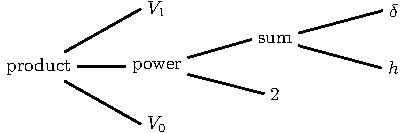
\includegraphics{img/chapter2/sage_operations/tree.pdf}
    \end{center}
    \caption{A possible tree of operations for $V_1 (\delta+h)^2 V_0$.}\label{fig:c2_operations_tree}
\end{figure}

Now we can write an expression such as $V_1 (\delta + h)^2 V_0$, which \sage{} would immediately translate to the expanded expression:
$$
    V_{0} V_{1} \delta^{2} + 2 V_{0} V_{1} h \delta + V_{0} V_{1} h^{2}\text{.}
$$
This expression is much more efficient to work with. For the first expression, a computer algebra system has to save this as a tree of operations, see figure \ref{fig:c2_operations_tree}. This tree is cumbersome and relatively slow to work with. By specifying all variables to be polynomials, \sage{} can save these much more efficiently as a few simple arrays. For small expressions the difference may be negligible. But for the giant expressions we are working with, the difference is very significant.

Besides the computational benefit, we also have the ability to easily specify that $V_0, \dots, V_N$ are matrices when generating formulae for the constant perturbation method on coupled systems of equations. We do not specify $V_0, \dots, V_N$ to be in a polynomial ring, but a general free algebra without commutation rules.
%\begin{noindent}
\begin{minted}{python}
FreeAlgebra(QQ, ['V0', 'V1', 'V2'])
\end{minted}
%\end{noindent}
An expression such as $(V_1 + V_0)^2$ will now internally be stored as:
$$
    V_{0}^{2} + V_{0} V_{1} + V_{1} V_{0} + V_{1}^{2}\text{.}
$$

Using these polynomial rings it is straightforward to implement the formulae from theorem \ref{the:c2_perturbation_terms}. The last thing to do is generating the \cpp{}-code to compute the values $d_{q,i}$ from \eqref{equ:c2_symbolic_propagators}. For this we generate for each element of the propagation matrix $u(\delta)$, $v(\delta)$, $u'(\delta)$ and $v'(\delta)$ the $(Q+2)\times (N+1)$ matrix $T_p$ of formulae for $d_{q,i}$. For example:
$$
    (T_v)_{1, 3} = h\cdot\left(-0.5 V_1 + h\cdot\left(0.5 V_2 + h\cdot\left(-0.5 V_3 + h\cdot\left(\dots\right)\right)\right)\right)\text{.}
$$

As one may expect, this generates a huge file of code. In figure \ref{fig:c2_generated_code} we have provided the cleaned-up\footnote{In practice, we have to ensure all scalars have the right type, see section \ref{sec:c2_generalizing_scalar}. So a simple fraction like $\frac{37}{80}$ has to be implemented as \mintinline{c++}{Scalar(37LL)/Scalar(80LL)}, here is \texttt{Scalar} a template type variable.} generated code for $(T_u)_{4, 10}$. This expression is one example of the over $300$ complicated terms needed to generate the propagation matrix.

\begin{figure}
    %\begin{noindent}
\begin{minted}{python}
Tu[4, 10] = (
  37/80*v1*v1*v2 - 1065/56*v3*v3 - 165/4*v2*v4 - 261/4*v1*v5
  + 19305/2*v8
  + h*(-279/80*v1*v2*v2 - 69/16*v1*v1*v3
  + 945/2*v3*v4 + 567*v2*v5 + 891*v1*v6 - 328185/2*v9
  + h*(-7/192*v1*v1*v1*v1 + 39/8*v2*v2*v2 + 691/20*v1*v2*v3
  + 185/8*v1*v1*v4 - 12405/8*v4*v4 - 13251/4*v3*v5
  - 16731/4*v2*v6 - 26235/4*v1*v7 + 2953665/2*v10
  + h*(31/96*v1*v1*v1*v2 - 513/10*v2*v2*v3 - 953/16*v1*v3*v3
  - 1061/8*v1*v2*v4 - 735/8*v1*v1*v5 + 15120*v4*v5
  + 16956*v3*v6 + 21978*v2*v7 + 137709/4*v1*v8 - 18706545/2*v11
  + h*(-43/48*v1*v1*v2*v2 - 2/3*v1*v1*v1*v3 + 11427/80*v2*v3*v3
  + 12517/80*v2*v2*v4 + 1443/4*v1*v3*v4 + 1697/4*v1*v2*v5
  + 4781/16*v1*v1*v6 - 57765/2*v5*v5 - 60447*v4*v6 - 70110*v3*v7
  - 92169*v2*v8 - 144144*v1*v9 + 93532725/2*v12
  + h*(-1/3840*v1*v1*v1*v1*v1 + 31/32*v1*v2*v2*v2
  + 313/96*v1*v1*v2*v3 + 61/48*v1*v1*v1*v4 - 1809/16*v3*v3*v3
  - 2943/4*v2*v3*v4 - 7319/16*v1*v4*v4 - 34047/80*v2*v2*v5
  - 7811/8*v1*v3*v5 - 11823/10*v1*v2*v6 - 67137/80*v1*v1*v7
  + 192726*v5*v6 + 208521*v4*v7 + 247401*v3*v8 + 1311453/4*v2*v9
  + 2045043/4*v1*v10 - 392837445/2*v13
  + h*(1/768*v1*v1*v1*v1*v2
  - 23/64*v2*v2*v2*v2 - 77/16*v1*v2*v2*v3 - 517/192*v1*v1*v3*v3
  - 181/32*v1*v1*v2*v4 - 217/96*v1*v1*v1*v5 + 6161/8*v3*v3*v4
  + 13289/16*v2*v4*v4 + 14079/8*v2*v3*v5 + 8655/4*v1*v4*v5
  + 21051/20*v2*v2*v6 + 9605/4*v1*v3*v6 + 118279/40*v1*v2*v7
  + 33663/16*v1*v1*v8 - 558747/2*v6*v6 - 577323*v5*v7
  - 640332*v4*v8 - 771309*v3*v9 - 1027026*v2*v10
  - 1594593*v1*v11
)))))))
\end{minted}
%\end{noindent}
    \caption{The $\delta$-dependent formula for term $(T_u)_{4, 10}$, with $Q = 7$ and $N = 16$ as used by \matslise{3}. In reality this is only one of the over $300$ terms needed to compute the propagation matrix, with each term just as complicated as this one.}\label{fig:c2_generated_code}
\end{figure}

To aid the compiler, before generating the code, we implement a crude common subexpression elimination in \sage{}. Because we are working in a multivariate polynomial ring (or a free algebra in the case of coupled systems), expressions which are the product of some $V_i$'s such as  $V_1^2 V_2$ will be common. And, many of them will be present in more than one formula. We can start the code generation by extracting some of these products in their own variables. For example:
%\begin{noindent}
\begin{minted}{python}
...
v1_v2 = v1 * v2
v1_v1_v2 = v1 * v1_v2
...
\end{minted}
%\end{noindent}

In the scalar case, this works wonderfully. All tested compilers are able to process this generated file without many difficulties. For coupled systems this generated file is much harder on the compiler because $V_0, \dots, V_N$ are no longer simple scalars. They have become matrices from the \Eigen{} library. \Eigen{} relies upon inlining and other compiler optimizations to generate the best possible machine-code, for some compilers (most notably for the Microsoft Visual Studio compiler) this becomes too much, and they run out of available system memory. To combat this issue partially, we introduce more temporaries and split the giant formulas into more manageable simpler expressions.

\subsubsection{Generalizing the scalar-type}\label{sec:c2_generalizing_scalar}

One of the very cool features of the linear algebra library \Eigen is that it does not care what kind of scalars you are working with. All their algorithms are implemented agnostic of the scalar type. This is achieved by using \cpp{}-templates. For readers unfamiliar with this concept we will provide a very brief summary of this concept. For a thorough description see \cite[Chapter~23]{stroustrup_programming_2013}.

First, let us take a look at the \texttt{C}-functions to compute the square root of a floating point number.
% \begin{noindent}
\begin{minted}{C}
float sqrtf(float arg);
double sqrt(double arg);
long double sqrtl(long double arg);
\end{minted}
% \end{noindent}

The \texttt{C}-standard has to provide three different functions for three different floating point types: \texttt{float} is $32$ bits wide, \texttt{double} is $64$ bits wide and \texttt{long double} is commonly\footnote{The \texttt{C} and \cpp-standards give surprisingly vague definitions of numeric types. For example: the \texttt{int}-type is guaranteed to be \emph{at least} $16$ bits wide. The two floating point types \texttt{float} and \texttt{double} are atypical in the sense that they are guaranteed to be the IEEE-754 binary32 and binary64 formats respectively. For the \texttt{long double} type, the specification is less strict: \emph{``extended precision floating-point type. Matches IEEE-754 binary128 format if supported, otherwise matches IEEE-754 binary64-extended format if supported, otherwise matches some non-IEEE-754 extended floating-point format as long as its precision is better than binary64 and range is at least as good as binary64, otherwise matches IEEE-754 binary64 format.''} On x86 systems, this is an $80$ bit wide floating point type with a 15 bits exponent and 64 bits significand.} $80$ bits wide.

It is cumbersome to have to differentiate between which function to call, depending on which argument types are used. In \cpp{} this is solved more elegantly, by allowing function overloads depending on the supplied arguments. But \cpp{} goes even further, a programmer can build a function for different types with the same code. For example, the following code implements the simple operations $x^2 + y^2$, for all possible types all at once.
% \begin{noindent}
\begin{minted}{c++}
template<typename Number>
Number squared_norm(Number x, Number y) {
    Number a = x * x;
    Number b = y * y;
    return a + b;
}
\end{minted}
% \end{noindent}
This function can now be called with different numeric types.
% \begin{noindent}
\begin{minted}{c++}
squared_norm<int>(3, 4);
squared_norm<float>(3.0f, 4.0f);
squared_norm<double>(3.0, 4.0);
\end{minted}
% \end{noindent}

The library \Eigen{} is implemented by using these templates extensively. This library provides the \texttt{Eigen::Matrix<Scalar, rows, cols>} type which can be used to build for example the following matrices.
% \begin{noindent}
\begin{minted}{c++}
// A 3 by 3 integer matrix
Eigen::Matrix<int, 3, 3>
\end{minted}
\begin{minted}{c++}
// A double-type column vector with a dynamic number of rows
Eigen::Matrix<double, Eigen::Dynamic, 1>
\end{minted}
\begin{minted}{c++}
// A complex 10 by 5 matrix, the real and imaginary part of
// each entry is saved in a long double format.
Eigen::Matrix<std::complex<long double>, 10, 5> 
\end{minted}
% \end{noindent}

\begin{figure}
    % \begin{noindent}
\begin{minted}{c++}
#include <iostream>
#include <boost/format.hpp>
#include <boost/math/constants/constants.hpp>
#include <boost/multiprecision/float128.hpp>
#include <matslise/matslise.h>

using boost::math::constants::pi;
using boost::multiprecision::float128;

float128 mathieuPotential(float128 x) {
    return 2 * cos(2 * x);
}

int main() {
    matslise::Matslise<float128> problem(
            &mathieuPotential, 0, pi<float128>(), 1e-25q);

    auto boundary = matslise::Y<float128>::Dirichlet();
    auto eigs = problem.eigenvaluesByIndex(0, 7, boundary);
    for (auto [i, E]: eigs) {
        float128 error = problem.eigenvalueError(E, boundary, i);
        std::cout << boost::format(
                "Eigenvalue %1$d:%2$30.25f  (error: %3$.1e)")
                        % i % E % error << std::endl;
    }
    return 0;
}
\end{minted}
% \end{noindent}
    \vspace{8mm}
    % \begin{noindent}
\begin{minted}{text}
Eigenvalue 0:  -0.1102488169920951699065478  (error: 1.7e-25)
Eigenvalue 1:   3.9170247729984711867034169  (error: 1.6e-25)
Eigenvalue 2:   9.0477392598093749823749465  (error: 1.9e-25)
Eigenvalue 3:  16.0329700814057944092457252  (error: 4.3e-25)
Eigenvalue 4:  25.0208408232897663652258825  (error: 4.8e-25)
Eigenvalue 5:  36.0142899106282223466625724  (error: 7.7e-25)
Eigenvalue 6:  49.0104182494238719005911294  (error: 9.8e-25)
\end{minted}
% \end{noindent}
    \caption{A sample program to compute the first 8 eigenvalues of the Mathieu problem from section \ref{sec:c2_numerical_experiments_mathieu} in $128$ bits wide floating point precision, and the output generated.}
    \label{fig:c2_mathieu_quad_code}
\end{figure}

In our implementation we have also adopted this philosophy by using templates to allow for any scalar type. This means that \matslise{3} is not only able to solve Sturm-Liouville equations in \texttt{double}-precision (like \matslise{2}) but also in the more accurate \texttt{long double}-precision. We even have enabled support for a $128$ bits floating point  numeric type by using Boost's \cite{boost_float128_} \texttt{boost::multiprecision::float128} type.

Unfortunately, \lpython{} only has support for the double type. So, if we want to leverage this higher precision, we will have to write a \cpp{} program. As an example, in figure \ref{fig:c2_mathieu_quad_code} we provide the code to find the first few eigenvalues of the Mathieu problem from section \ref{sec:c2_numerical_experiments_mathieu} in quadruple precision ($128$ bit).

\subsubsection{Memory management}

In computer science, a garbage collector is a method to do automatic memory management. The idea here is to automatically detect if allocated memory (for an array or object for example) is no longer used. If such memory is found, this can be returned to the operating system, for later use by our own or another program. Detecting unused memory is essential to ensure a reliable working of the system. If one program hoards memory, without returning it to the operating system, then sooner or later the operating system runs out of memory and programs need to be unexpectedly aborted.

To avoid this, many interpreted languages (for example \lpython{}, \javascript{}, \matlab{}\dots) have such a garbage collector build in. Even some compiled languages (such as \java{} or \csharp{}) do memory management with a garbage collector. But this is not the only way to manage memory, \rust{} for example, keeps track of which memory is used at compile time with what they call \emph{lifetimes}. \texttt{C} and \cpp{} on the other hand, have no memory management build in, these languages rely on the programmer to clean up after themselves.

In theory, cleaning up after yourself is easy. When you allocate data, just make sure you deallocate it once you no longer need it. In practice, this view is too simple. In \cpp{} some memory management is handled automatically by constructors and destructors. But other, more complicated scenarios, still have to be handled by the programmer. The situation that caused problems was the interoperability with \lpython{}. We had to very carefully specify whose responsibility it was to clean up objects. Was it an object that was managed on the \cpp{} side by us, the programmer, or could we let the garbage collector of \lpython{} do the work? Luckily, \pybind{} supports \texttt{std::shared\_ptr<...>}, using this solves the responsibility issue in most cases.

The only problematic case left, is when the lifetime of one object depends upon another object. For example consider the following \lpython{} code, which computes and stores the sixth eigenfunction of three different Schrödinger problems.
% \begin{noindent}
\begin{minted}{python3}
from pyslise import Pyslise

some_functions = []
for q in [1, 10, 100]:
    problem = Pyslise(lambda x: q*x, 0, 1)
    i, E, f = problem.eigenpairsByIndex(5, 6, (0, 1))[0]
    some_functions.append(f)
\end{minted}
% \end{noindent}
Here, in the body of the loop, the eigenfunction object \texttt{f} assumes that the original \texttt{Pyslise} object \texttt{problem} exists. If \texttt{problem} were destroyed, evaluating the eigenfunction \texttt{f} would trigger undefined behavior. In the best case, this would crash the program, in the worst case wrong results would be returned. To ensure \texttt{problem} not to be destroyed to early we have to explicitly mark a dependence of each of the returned eigenfunctions on the original problem.

In hindsight, these issues and fixes may seem obvious. But, they highlight some difficulties in getting \lpython{} and \cpp{} to play nicely together.

\subsubsection{Automatic testing}

Another challenge we want to focus on is an often underappreciated issue in mathematical software development. When programming there is an almost universal truth: all software contains bugs. An art in writing software is maximizing the chance you catch bugs early. One of the best tools available for this is automatic tests. These tests should be extremely easy to run and require no input from the programmer whatsoever. They should just result in a pass/fail condition. Using a well established test framework makes writing tests a breeze, and encourages implementing more tests when new functionality is added or when new edge-cases are discovered.

We have chosen to use \catch{} \cite{_catchorg_2023} as a test framework. And, implemented $43$ test scenarios with over $\numprint{2000000}$ conditions to check. These tests range from simple unit-tests to ensure the Legendre-polynomials are computed correctly or that our program is able to evaluate the $\eta_i$ functions in all floating point types, to full integration tests where a Sturm-Liouville problem is solved, and the accuracy is verified. As a summary we provide a small description of some of these automatic tests.

\begin{itemize}
    \item Some simple unit-tests of some auxiliary procedures \begin{itemize}
              \item Least squares approximations of trigonometric functions with shifted Legendre polynomials
              \item The evaluation of the $\eta_i$-funtions in many points for all scalar types.
              \item The domain and the Schrödinger potential after Liouville's transformation applied to $p(x) = \cos(x)$, $q(x) = 0$ and $w(x) = \tan(x) \sin(x)$.
          \end{itemize}
    \item Some Sturm-Liouville problems with exact known eigenvalues \begin{itemize}
              \item The Schrödinger problem with $V(x) = 0$ on $\left[-\frac{\pi}{2}, \frac{\pi}{2}\right]$ with homogeneous Dirichlet boundary conditions. The first $50$ eigenfunctions are compared in many points to the analytical solution.
              \item The Schrödinger problem with $V(x) = x^2$ on $\left[-15, 15\right]$ with homogeneous Dirichlet boundary conditions. The first $50$ eigenvalues and the orthonormality of the eigenfunctions are verified, in \texttt{double}, \texttt{long double} and \texttt{float128}.
              \item Klotter's problem\cite{klotter_technische_1978} with $p(x) = 1$, $q(x) = \frac{3}{4x^2}$ and $w(x) = \frac{64\pi^2}{9 x^6}$ on $\left[\frac{8}{7}, 8\right]$.
          \end{itemize}
    \item Some Schrödinger problems with eigenvalues found in the literature and with \matslise{2}\begin{itemize}
              \item The Mathieu problem $V(x)= 2\cos(2x)$ on $[0, \pi]$. The first $200$ eigenvalues and the orthonormality of the eigenfunctions are checked, in \texttt{double}, \texttt{long double} and \texttt{float128}. The first and fourth eigenfunctions are compared in different values computed with \matslise{2}.
              \item Marletta's problem: $V(x) = 3\frac{x-31}{4(x+1)(x+4)^2}$ on $[0,12]$ with $y(0) = 0$ and $5 y(12) + 8 y'(12) = 0$.
              \item The Coffey-Evans problem: $V(x) = -2 \beta \cos(2x) + \beta^2 \sin^2(2x)$ on $\left[-\frac{\pi}{2}, \frac{\pi}{2}\right]$ with homogeneous Dirichlet boundary conditions and half-range reduction for $\beta \in \{20, 25\}$ with all scalar types.
          \end{itemize}
    \item Sturm-Liouville problems from \cite{siedlecki_sturmliouville_2016} are checked to their reported values. For the second and third problem, the reported results in \cite{siedlecki_sturmliouville_2016} are not as accurate as we desire, so \matslise{2} was used to provide more accurate values.
          \begin{itemize}
              \item $p(x)=1$, $q(x)=0$ and $w(x)=(1+x)^{-2}$ with homogeneous Dirichlet boundary conditions on $[0, 1]$.
              \item $p=(1+x)^1$, $q(x) = x^2-2$ and $w(x) = \exp(x)$ on $[0, 1]$ with homogeneous Dirichlet boundary conditions left and homogeneous Neumann conditions on the right.
              \item $p(x) = 2+\sin(2 \pi x)$, $q(x) = -10$ and $w(x) = 1+\sqrt{x}$ on $[0, 1]$ with boundary conditions $y(0) = 0$ and $10 y(1) + p(1) y'(1) = 0$. The first three eigenfunctions are also compared to values computed with \matslise{2}.
          \end{itemize}
    \item The following Schrödinger problems with periodic boundary conditions from \cite{andrew_correction_1989}.
          \begin{itemize}
              \item The first $20$ eigenvalues of the periodic problem with potential $V(x) = x^2(\pi - x)$.
              \item For $V(x) = x^2(\pi - x)$ a selection of eigenvalues with index up to $40$.
          \end{itemize}
\end{itemize}

All these tests can be easily run during development. They are automatically run on each code change with the help of GitHub Actions. Here the program is compiled, and the tests are executed on a clean test system on GitHub's servers for Linux, macOS and Windows. This also builds and tests the Python-package. Working with GitHub Actions for automated testing allows us to quickly detect code regressions and failing tests on other operating system.

\subsection{A graphical user interface}\label{sec:c2_online_gui}

\todo{Expand this section, maybe add a screenshot}

Since all the code is written in \texttt{C++} it can be compiled to WebAssembly. This format enables most modern browsers to execute the code, this has been tested in Firefox and Chrome. Of course this will not be as efficient as running it natively through \texttt{C++} or Python.

\section{Conclusions and future work}

\todo{Write a conclusion}

\begin{enumerate}
    \item What have we added, what is new?
    \item Dynamically expanding domains.
\end{enumerate}

\stopchapter
